\documentclass[%
 reprint,
%superscriptaddress,
%groupedaddress,
%unsortedaddress,
%runinaddress,
%frontmatterverbose, 
%preprint,
%showpacs,preprintnumbers,
%nofootinbib,
%nobibnotes,
%bibnotes,
 amsmath,amssymb,
 aps, prl
]{revtex4-1}

\usepackage{graphicx}% Include figure files
\usepackage{dcolumn}% Align table columns on decimal point
\usepackage{bm}% bold math
\usepackage{hyperref}% add hypertext capabilities
%\usepackage[mathlines]{lineno}% Enable numbering of text and display math
%\linenumbers\relax % Commence numbering lines

% --- LHCb specfic ----
\usepackage{ifthen} % for conditional statements
\newboolean{pdflatex}
\setboolean{pdflatex}{true} % False for eps figures 

\newboolean{articletitles}
\setboolean{articletitles}{true} % False removes titles in references

\newboolean{uprightparticles}
\setboolean{uprightparticles}{false} %True for upright particle symbols

\newboolean{inbibliography}
\setboolean{inbibliography}{false} %True once you enter the bibliography

\newboolean{wordcount}
\setboolean{wordcount}{false} % False for normal usage; true for wordcount.sh

\ifthenelse{\boolean{wordcount}}%
{\usepackage{bibentry} % For nobibliography command
 \usepackage{mciteplus} % combine multiple citations
 \usepackage{comment} % comment lines
 % Uncomment the lines below to exclude equations from the word count
 %\excludecomment{align*} % Remove align*
 %\excludecomment{align} % Remove align
 %\let\endalign\relax % Remove align
 %\excludecomment{equation*} % Remove equation* (does not work)
 %\excludecomment{equation} % Remove equation
 %\let\endequation\relax % Remove equation
 %\excludecomment{eqnarray*} % Remove eqnarray*
 %\excludecomment{eqnarray} % Remove eqnarray
 %\let\endeqnarray\relax % Remove eqnarray
 \excludecomment{acknowledgments} % Remove acknowledgments
 \let\endacknowledgments\relax % Remove acknowledgments
 \def\maketitle{} % Remove title and abstract
}{
}

\graphicspath{{./figs/}}
\DeclareGraphicsExtensions{.pdf,.PDF,png,.PNG}
\usepackage{xspace} 
\makeatletter
\gdef\@ptsize{0} % fix miniscule font definition from lhcb-symbols
\makeatother
\let\put\relax % avoid \put commands in a PRL paper 
% Remove the Acknowledgement heading for PRL
\makeatletter
\usepackage{suffix}
\let\latex@section\section
\WithSuffix\def\section*{\secdef\my@section{\latex@section*}}
\def\my@section[#1]#2{}
\makeatother

%%% $Id: lhcb-symbols-def.tex 90362 2016-04-07 13:38:32Z pkoppenb $
%%% ======================================================================
%%% Purpose: Standard LHCb aliases
%%% Author: Originally Ulrik Egede, adapted by Tomasz Skwarnicki for templates,
%%% rewritten by Chris Parkes
%%% Maintainer : Ulrik Egede (2010 - 2012)
%%% Maintainer : Rolf Oldeman (2012 - 2014)
%%% =======================================================================

%%% To use this file outside the normal LHCb document environment, the
%%% following should be added in a preamble (before \begin{document}
%%%
%%%\usepackage{ifthen} 
%%%\newboolean{uprightparticles}
%%%\setboolean{uprightparticles}{false} %Set true for upright particle symbols
\usepackage{xspace} 
\usepackage{upgreek}

%%%%%%%%%%%%%%%%%%%%%%%%%%%%%%%%%%%%%%%%%%%%%%%%%%%%%%%%%%%%
%%%
%%% The following is to ensure that the template automatically can process
%%% this file.
%%%
%%% Add comments with at least three %%% preceding.
%%% Add new sections with one % preceding
%%% Add new subsections with two %% preceding
%%%%%%%%%%%%%%%%%%%%%%%%%%%%%%%%%%%%%%%%%%%%%%%%%%%%%%%%%%%%

%%%%%%%%%%%%%
% Experiments
%%%%%%%%%%%%%
\def\lhcb {\mbox{LHCb}\xspace}
\def\atlas  {\mbox{ATLAS}\xspace}
\def\cms    {\mbox{CMS}\xspace}
\def\alice  {\mbox{ALICE}\xspace}
\def\babar  {\mbox{BaBar}\xspace}
\def\belle  {\mbox{Belle}\xspace}
\def\cleo   {\mbox{CLEO}\xspace}
\def\cdf    {\mbox{CDF}\xspace}
\def\dzero  {\mbox{D0}\xspace}
\def\aleph  {\mbox{ALEPH}\xspace}
\def\delphi {\mbox{DELPHI}\xspace}
\def\opal   {\mbox{OPAL}\xspace}
\def\lthree {\mbox{L3}\xspace}
\def\sld    {\mbox{SLD}\xspace}
%%%\def\argus  {\mbox{ARGUS}\xspace}
%%%\def\uaone  {\mbox{UA1}\xspace}
%%%\def\uatwo  {\mbox{UA2}\xspace}
%%%\def\ux85 {\mbox{UX85}\xspace}
\def\cern {\mbox{CERN}\xspace}
\def\lhc    {\mbox{LHC}\xspace}
\def\lep    {\mbox{LEP}\xspace}
\def\tevatron {Tevatron\xspace}

%% LHCb sub-detectors and sub-systems

%%%\def\pu     {PU\xspace}
\def\velo   {VELO\xspace}
\def\rich   {RICH\xspace}
\def\richone {RICH1\xspace}
\def\richtwo {RICH2\xspace}
\def\ttracker {TT\xspace}
\def\intr   {IT\xspace}
\def\st     {ST\xspace}
\def\ot     {OT\xspace}
%%%\def\Tone   {T1\xspace}
%%%\def\Ttwo   {T2\xspace}
%%%\def\Tthree {T3\xspace}
%%%\def\Mone   {M1\xspace}
%%%\def\Mtwo   {M2\xspace}
%%%\def\Mthree {M3\xspace}
%%%\def\Mfour  {M4\xspace}
%%%\def\Mfive  {M5\xspace}
\def\spd    {SPD\xspace}
\def\presh  {PS\xspace}
\def\ecal   {ECAL\xspace}
\def\hcal   {HCAL\xspace}
%%%\def\bcm    {BCM\xspace}
\def\MagUp {\mbox{\em Mag\kern -0.05em Up}\xspace}
\def\MagDown {\mbox{\em MagDown}\xspace}

\def\ode    {ODE\xspace}
\def\daq    {DAQ\xspace}
\def\tfc    {TFC\xspace}
\def\ecs    {ECS\xspace}
\def\lone   {L0\xspace}
\def\hlt    {HLT\xspace}
\def\hltone {HLT1\xspace}
\def\hlttwo {HLT2\xspace}

%%% Upright (not slanted) Particles

\ifthenelse{\boolean{uprightparticles}}%
{\def\Palpha      {\ensuremath{\upalpha}\xspace}
 \def\Pbeta       {\ensuremath{\upbeta}\xspace}
 \def\Pgamma      {\ensuremath{\upgamma}\xspace}                 
 \def\Pdelta      {\ensuremath{\updelta}\xspace}                 
 \def\Pepsilon    {\ensuremath{\upepsilon}\xspace}                 
 \def\Pvarepsilon {\ensuremath{\upvarepsilon}\xspace}                 
 \def\Pzeta       {\ensuremath{\upzeta}\xspace}                 
 \def\Peta        {\ensuremath{\upeta}\xspace}                 
 \def\Ptheta      {\ensuremath{\uptheta}\xspace}                 
 \def\Pvartheta   {\ensuremath{\upvartheta}\xspace}                 
 \def\Piota       {\ensuremath{\upiota}\xspace}                 
 \def\Pkappa      {\ensuremath{\upkappa}\xspace}                 
 \def\Plambda     {\ensuremath{\uplambda}\xspace}                 
 \def\Pmu         {\ensuremath{\upmu}\xspace}                 
 \def\Pnu         {\ensuremath{\upnu}\xspace}                 
 \def\Pxi         {\ensuremath{\upxi}\xspace}                 
 \def\Ppi         {\ensuremath{\uppi}\xspace}                 
 \def\Pvarpi      {\ensuremath{\upvarpi}\xspace}                 
 \def\Prho        {\ensuremath{\uprho}\xspace}                 
 \def\Pvarrho     {\ensuremath{\upvarrho}\xspace}                 
 \def\Ptau        {\ensuremath{\uptau}\xspace}                 
 \def\Pupsilon    {\ensuremath{\upupsilon}\xspace}                 
 \def\Pphi        {\ensuremath{\upphi}\xspace}                 
 \def\Pvarphi     {\ensuremath{\upvarphi}\xspace}                 
 \def\Pchi        {\ensuremath{\upchi}\xspace}                 
 \def\Ppsi        {\ensuremath{\uppsi}\xspace}                 
 \def\Pomega      {\ensuremath{\upomega}\xspace}                 

 \def\PDelta      {\ensuremath{\Delta}\xspace}                 
 \def\PXi      {\ensuremath{\Xi}\xspace}                 
 \def\PLambda      {\ensuremath{\Lambda}\xspace}                 
 \def\PSigma      {\ensuremath{\Sigma}\xspace}                 
 \def\POmega      {\ensuremath{\Omega}\xspace}                 
 \def\PUpsilon      {\ensuremath{\Upsilon}\xspace}                 
 
 %\mathchardef\Deltares="7101
 %\mathchardef\Xi="7104
 %\mathchardef\Lambda="7103
 %\mathchardef\Sigma="7106
 %\mathchardef\Omega="710A


 \def\PA      {\ensuremath{\mathrm{A}}\xspace}                 
 \def\PB      {\ensuremath{\mathrm{B}}\xspace}                 
 \def\PC      {\ensuremath{\mathrm{C}}\xspace}                 
 \def\PD      {\ensuremath{\mathrm{D}}\xspace}                 
 \def\PE      {\ensuremath{\mathrm{E}}\xspace}                 
 \def\PF      {\ensuremath{\mathrm{F}}\xspace}                 
 \def\PG      {\ensuremath{\mathrm{G}}\xspace}                 
 \def\PH      {\ensuremath{\mathrm{H}}\xspace}                 
 \def\PI      {\ensuremath{\mathrm{I}}\xspace}                 
 \def\PJ      {\ensuremath{\mathrm{J}}\xspace}                 
 \def\PK      {\ensuremath{\mathrm{K}}\xspace}                 
 \def\PL      {\ensuremath{\mathrm{L}}\xspace}                 
 \def\PM      {\ensuremath{\mathrm{M}}\xspace}                 
 \def\PN      {\ensuremath{\mathrm{N}}\xspace}                 
 \def\PO      {\ensuremath{\mathrm{O}}\xspace}                 
 \def\PP      {\ensuremath{\mathrm{P}}\xspace}                 
 \def\PQ      {\ensuremath{\mathrm{Q}}\xspace}                 
 \def\PR      {\ensuremath{\mathrm{R}}\xspace}                 
 \def\PS      {\ensuremath{\mathrm{S}}\xspace}                 
 \def\PT      {\ensuremath{\mathrm{T}}\xspace}                 
 \def\PU      {\ensuremath{\mathrm{U}}\xspace}                 
 \def\PV      {\ensuremath{\mathrm{V}}\xspace}                 
 \def\PW      {\ensuremath{\mathrm{W}}\xspace}                 
 \def\PX      {\ensuremath{\mathrm{X}}\xspace}                 
 \def\PY      {\ensuremath{\mathrm{Y}}\xspace}                 
 \def\PZ      {\ensuremath{\mathrm{Z}}\xspace}                 
 \def\Pa      {\ensuremath{\mathrm{a}}\xspace}                 
 \def\Pb      {\ensuremath{\mathrm{b}}\xspace}                 
 \def\Pc      {\ensuremath{\mathrm{c}}\xspace}                 
 \def\Pd      {\ensuremath{\mathrm{d}}\xspace}                 
 \def\Pe      {\ensuremath{\mathrm{e}}\xspace}                 
 \def\Pf      {\ensuremath{\mathrm{f}}\xspace}                 
 \def\Pg      {\ensuremath{\mathrm{g}}\xspace}                 
 \def\Ph      {\ensuremath{\mathrm{h}}\xspace}                 
 \def\Pi      {\ensuremath{\mathrm{i}}\xspace}                 
 \def\Pj      {\ensuremath{\mathrm{j}}\xspace}                 
 \def\Pk      {\ensuremath{\mathrm{k}}\xspace}                 
 \def\Pl      {\ensuremath{\mathrm{l}}\xspace}                 
 \def\Pm      {\ensuremath{\mathrm{m}}\xspace}                 
 \def\Pn      {\ensuremath{\mathrm{n}}\xspace}                 
 \def\Po      {\ensuremath{\mathrm{o}}\xspace}                 
 \def\Pp      {\ensuremath{\mathrm{p}}\xspace}                 
 \def\Pq      {\ensuremath{\mathrm{q}}\xspace}                 
 \def\Pr      {\ensuremath{\mathrm{r}}\xspace}                 
 \def\Ps      {\ensuremath{\mathrm{s}}\xspace}                 
 \def\Pt      {\ensuremath{\mathrm{t}}\xspace}                 
 \def\Pu      {\ensuremath{\mathrm{u}}\xspace}                 
 \def\Pv      {\ensuremath{\mathrm{v}}\xspace}                 
 \def\Pw      {\ensuremath{\mathrm{w}}\xspace}                 
 \def\Px      {\ensuremath{\mathrm{x}}\xspace}                 
 \def\Py      {\ensuremath{\mathrm{y}}\xspace}                 
 \def\Pz      {\ensuremath{\mathrm{z}}\xspace}                 
}
{\def\Palpha      {\ensuremath{\alpha}\xspace}
 \def\Pbeta       {\ensuremath{\beta}\xspace}
 \def\Pgamma      {\ensuremath{\gamma}\xspace}                 
 \def\Pdelta      {\ensuremath{\delta}\xspace}                 
 \def\Pepsilon    {\ensuremath{\epsilon}\xspace}                 
 \def\Pvarepsilon {\ensuremath{\varepsilon}\xspace}                 
 \def\Pzeta       {\ensuremath{\zeta}\xspace}                 
 \def\Peta        {\ensuremath{\eta}\xspace}                 
 \def\Ptheta      {\ensuremath{\theta}\xspace}                 
 \def\Pvartheta   {\ensuremath{\vartheta}\xspace}                 
 \def\Piota       {\ensuremath{\iota}\xspace}                 
 \def\Pkappa      {\ensuremath{\kappa}\xspace}                 
 \def\Plambda     {\ensuremath{\lambda}\xspace}                 
 \def\Pmu         {\ensuremath{\mu}\xspace}                 
 \def\Pnu         {\ensuremath{\nu}\xspace}                 
 \def\Pxi         {\ensuremath{\xi}\xspace}                 
 \def\Ppi         {\ensuremath{\pi}\xspace}                 
 \def\Pvarpi      {\ensuremath{\varpi}\xspace}                 
 \def\Prho        {\ensuremath{\rho}\xspace}                 
 \def\Pvarrho     {\ensuremath{\varrho}\xspace}                 
 \def\Ptau        {\ensuremath{\tau}\xspace}                 
 \def\Pupsilon    {\ensuremath{\upsilon}\xspace}                 
 \def\Pphi        {\ensuremath{\phi}\xspace}                 
 \def\Pvarphi     {\ensuremath{\varphi}\xspace}                 
 \def\Pchi        {\ensuremath{\chi}\xspace}                 
 \def\Ppsi        {\ensuremath{\psi}\xspace}                 
 \def\Pomega      {\ensuremath{\omega}\xspace}                 
 \mathchardef\PDelta="7101
 \mathchardef\PXi="7104
 \mathchardef\PLambda="7103
 \mathchardef\PSigma="7106
 \mathchardef\POmega="710A
 \mathchardef\PUpsilon="7107
 \def\PA      {\ensuremath{A}\xspace}                 
 \def\PB      {\ensuremath{B}\xspace}                 
 \def\PC      {\ensuremath{C}\xspace}                 
 \def\PD      {\ensuremath{D}\xspace}                 
 \def\PE      {\ensuremath{E}\xspace}                 
 \def\PF      {\ensuremath{F}\xspace}                 
 \def\PG      {\ensuremath{G}\xspace}                 
 \def\PH      {\ensuremath{H}\xspace}                 
 \def\PI      {\ensuremath{I}\xspace}                 
 \def\PJ      {\ensuremath{J}\xspace}                 
 \def\PK      {\ensuremath{K}\xspace}                 
 \def\PL      {\ensuremath{L}\xspace}                 
 \def\PM      {\ensuremath{M}\xspace}                 
 \def\PN      {\ensuremath{N}\xspace}                 
 \def\PO      {\ensuremath{O}\xspace}                 
 \def\PP      {\ensuremath{P}\xspace}                 
 \def\PQ      {\ensuremath{Q}\xspace}                 
 \def\PR      {\ensuremath{R}\xspace}                 
 \def\PS      {\ensuremath{S}\xspace}                 
 \def\PT      {\ensuremath{T}\xspace}                 
 \def\PU      {\ensuremath{U}\xspace}                 
 \def\PV      {\ensuremath{V}\xspace}                 
 \def\PW      {\ensuremath{W}\xspace}                 
 \def\PX      {\ensuremath{X}\xspace}                 
 \def\PY      {\ensuremath{Y}\xspace}                 
 \def\PZ      {\ensuremath{Z}\xspace}                 
 \def\Pa      {\ensuremath{a}\xspace}                 
 \def\Pb      {\ensuremath{b}\xspace}                 
 \def\Pc      {\ensuremath{c}\xspace}                 
 \def\Pd      {\ensuremath{d}\xspace}                 
 \def\Pe      {\ensuremath{e}\xspace}                 
 \def\Pf      {\ensuremath{f}\xspace}                 
 \def\Pg      {\ensuremath{g}\xspace}                 
 \def\Ph      {\ensuremath{h}\xspace}                 
 \def\Pi      {\ensuremath{i}\xspace}                 
 \def\Pj      {\ensuremath{j}\xspace}                 
 \def\Pk      {\ensuremath{k}\xspace}                 
 \def\Pl      {\ensuremath{l}\xspace}                 
 \def\Pm      {\ensuremath{m}\xspace}                 
 \def\Pn      {\ensuremath{n}\xspace}                 
 \def\Po      {\ensuremath{o}\xspace}                 
 \def\Pp      {\ensuremath{p}\xspace}                 
 \def\Pq      {\ensuremath{q}\xspace}                 
 \def\Pr      {\ensuremath{r}\xspace}                 
 \def\Ps      {\ensuremath{s}\xspace}                 
 \def\Pt      {\ensuremath{t}\xspace}                 
 \def\Pu      {\ensuremath{u}\xspace}                 
 \def\Pv      {\ensuremath{v}\xspace}                 
 \def\Pw      {\ensuremath{w}\xspace}                 
 \def\Px      {\ensuremath{x}\xspace}                 
 \def\Py      {\ensuremath{y}\xspace}                 
 \def\Pz      {\ensuremath{z}\xspace}                 
}

%%%%%%%%%%%%%%%%%%%%%%%%%%%%%%%%%%%%%%%%%%%%%%%
% Particles
\makeatletter
\ifcase \@ptsize \relax% 10pt
  \newcommand{\miniscule}{\@setfontsize\miniscule{4}{5}}% \tiny: 5/6
\or% 11pt
  \newcommand{\miniscule}{\@setfontsize\miniscule{5}{6}}% \tiny: 6/7
\or% 12pt
  \newcommand{\miniscule}{\@setfontsize\miniscule{5}{6}}% \tiny: 6/7
\fi
\makeatother


\DeclareRobustCommand{\optbar}[1]{\shortstack{{\miniscule (\rule[.5ex]{1.25em}{.18mm})}
  \\ [-.7ex] $#1$}}


%% Leptons

\let\emi\en
\def\electron   {{\ensuremath{\Pe}}\xspace}
\def\en         {{\ensuremath{\Pe^-}}\xspace}   % electron negative (\em is taken)
\def\ep         {{\ensuremath{\Pe^+}}\xspace}
\def\epm        {{\ensuremath{\Pe^\pm}}\xspace} 
\def\epem       {{\ensuremath{\Pe^+\Pe^-}}\xspace}
%%%\def\ee         {\ensuremath{\Pe^-\Pe^-}\xspace}

\def\muon       {{\ensuremath{\Pmu}}\xspace}
\def\mup        {{\ensuremath{\Pmu^+}}\xspace}
\def\mun        {{\ensuremath{\Pmu^-}}\xspace} % muon negative (\mum is taken)
\def\mumu       {{\ensuremath{\Pmu^+\Pmu^-}}\xspace}

\def\tauon      {{\ensuremath{\Ptau}}\xspace}
\def\taup       {{\ensuremath{\Ptau^+}}\xspace}
\def\taum       {{\ensuremath{\Ptau^-}}\xspace}
\def\tautau     {{\ensuremath{\Ptau^+\Ptau^-}}\xspace}

\def\lepton     {{\ensuremath{\ell}}\xspace}
\def\ellm       {{\ensuremath{\ell^-}}\xspace}
\def\ellp       {{\ensuremath{\ell^+}}\xspace}
\def\ellell     {\ensuremath{\ell^+ \ell^-}\xspace}

\def\neu        {{\ensuremath{\Pnu}}\xspace}
\def\neub       {{\ensuremath{\overline{\Pnu}}}\xspace}
%%%\def\nuenueb    {\ensuremath{\neu\neub}\xspace}
\def\neue       {{\ensuremath{\neu_e}}\xspace}
\def\neueb      {{\ensuremath{\neub_e}}\xspace}
%%%\def\neueneueb  {\ensuremath{\neue\neueb}\xspace}
\def\neum       {{\ensuremath{\neu_\mu}}\xspace}
\def\neumb      {{\ensuremath{\neub_\mu}}\xspace}
%%%\def\neumneumb  {\ensuremath{\neum\neumb}\xspace}
\def\neut       {{\ensuremath{\neu_\tau}}\xspace}
\def\neutb      {{\ensuremath{\neub_\tau}}\xspace}
%%%\def\neutneutb  {\ensuremath{\neut\neutb}\xspace}
\def\neul       {{\ensuremath{\neu_\ell}}\xspace}
\def\neulb      {{\ensuremath{\neub_\ell}}\xspace}
%%%\def\neulneulb  {\ensuremath{\neul\neulb}\xspace}

%% Gauge bosons and scalars

\def\g      {{\ensuremath{\Pgamma}}\xspace}
\def\H      {{\ensuremath{\PH^0}}\xspace}
\def\Hp     {{\ensuremath{\PH^+}}\xspace}
\def\Hm     {{\ensuremath{\PH^-}}\xspace}
\def\Hpm    {{\ensuremath{\PH^\pm}}\xspace}
\def\W      {{\ensuremath{\PW}}\xspace}
\def\Wp     {{\ensuremath{\PW^+}}\xspace}
\def\Wm     {{\ensuremath{\PW^-}}\xspace}
\def\Wpm    {{\ensuremath{\PW^\pm}}\xspace}
\def\Z      {{\ensuremath{\PZ}}\xspace}

%% Quarks

\def\quark     {{\ensuremath{\Pq}}\xspace}
\def\quarkbar  {{\ensuremath{\overline \quark}}\xspace}
\def\qqbar     {{\ensuremath{\quark\quarkbar}}\xspace}
\def\uquark    {{\ensuremath{\Pu}}\xspace}
\def\uquarkbar {{\ensuremath{\overline \uquark}}\xspace}
\def\uubar     {{\ensuremath{\uquark\uquarkbar}}\xspace}
\def\dquark    {{\ensuremath{\Pd}}\xspace}
\def\dquarkbar {{\ensuremath{\overline \dquark}}\xspace}
\def\ddbar     {{\ensuremath{\dquark\dquarkbar}}\xspace}
\def\squark    {{\ensuremath{\Ps}}\xspace}
\def\squarkbar {{\ensuremath{\overline \squark}}\xspace}
\def\ssbar     {{\ensuremath{\squark\squarkbar}}\xspace}
\def\cquark    {{\ensuremath{\Pc}}\xspace}
\def\cquarkbar {{\ensuremath{\overline \cquark}}\xspace}
\def\ccbar     {{\ensuremath{\cquark\cquarkbar}}\xspace}
\def\bquark    {{\ensuremath{\Pb}}\xspace}
\def\bquarkbar {{\ensuremath{\overline \bquark}}\xspace}
\def\bbbar     {{\ensuremath{\bquark\bquarkbar}}\xspace}
\def\tquark    {{\ensuremath{\Pt}}\xspace}
\def\tquarkbar {{\ensuremath{\overline \tquark}}\xspace}
\def\ttbar     {{\ensuremath{\tquark\tquarkbar}}\xspace}

%% Light mesons

\def\hadron {{\ensuremath{\Ph}}\xspace}
\def\pion   {{\ensuremath{\Ppi}}\xspace}
\def\piz    {{\ensuremath{\pion^0}}\xspace}
\def\pizs   {{\ensuremath{\pion^0\mbox\,\mathrm{s}}}\xspace}
\def\pip    {{\ensuremath{\pion^+}}\xspace}
\def\pim    {{\ensuremath{\pion^-}}\xspace}
\def\pipm   {{\ensuremath{\pion^\pm}}\xspace}
\def\pimp   {{\ensuremath{\pion^\mp}}\xspace}

\def\rhomeson {{\ensuremath{\Prho}}\xspace}
\def\rhoz     {{\ensuremath{\rhomeson^0}}\xspace}
\def\rhop     {{\ensuremath{\rhomeson^+}}\xspace}
\def\rhom     {{\ensuremath{\rhomeson^-}}\xspace}
\def\rhopm    {{\ensuremath{\rhomeson^\pm}}\xspace}
\def\rhomp    {{\ensuremath{\rhomeson^\mp}}\xspace}

\def\kaon    {{\ensuremath{\PK}}\xspace}
%%% do NOT use ensuremath here
  \def\Kbar    {{\kern 0.2em\overline{\kern -0.2em \PK}{}}\xspace}
\def\Kb      {{\ensuremath{\Kbar}}\xspace}
\def\KorKbar    {\kern 0.18em\optbar{\kern -0.18em K}{}\xspace}
\def\Kz      {{\ensuremath{\kaon^0}}\xspace}
\def\Kzb     {{\ensuremath{\Kbar{}^0}}\xspace}
\def\Kp      {{\ensuremath{\kaon^+}}\xspace}
\def\Km      {{\ensuremath{\kaon^-}}\xspace}
\def\Kpm     {{\ensuremath{\kaon^\pm}}\xspace}
\def\Kmp     {{\ensuremath{\kaon^\mp}}\xspace}
\def\KS      {{\ensuremath{\kaon^0_{\mathrm{ \scriptscriptstyle S}}}}\xspace}
\def\KL      {{\ensuremath{\kaon^0_{\mathrm{ \scriptscriptstyle L}}}}\xspace}
\def\Kstarz  {{\ensuremath{\kaon^{*0}}}\xspace}
\def\Kstarzb {{\ensuremath{\Kbar{}^{*0}}}\xspace}
\def\Kstar   {{\ensuremath{\kaon^*}}\xspace}
\def\Kstarb  {{\ensuremath{\Kbar{}^*}}\xspace}
\def\Kstarp  {{\ensuremath{\kaon^{*+}}}\xspace}
\def\Kstarm  {{\ensuremath{\kaon^{*-}}}\xspace}
\def\Kstarpm {{\ensuremath{\kaon^{*\pm}}}\xspace}
\def\Kstarmp {{\ensuremath{\kaon^{*\mp}}}\xspace}

\newcommand{\etaz}{\ensuremath{\Peta}\xspace}
\newcommand{\etapr}{\ensuremath{\Peta^{\prime}}\xspace}
\newcommand{\phiz}{\ensuremath{\Pphi}\xspace}
\newcommand{\omegaz}{\ensuremath{\Pomega}\xspace}

%% Heavy mesons

%%% do NOT use ensuremath here
  \def\Dbar    {{\kern 0.2em\overline{\kern -0.2em \PD}{}}\xspace}
\def\D       {{\ensuremath{\PD}}\xspace}
\def\Db      {{\ensuremath{\Dbar}}\xspace}
\def\DorDbar    {\kern 0.18em\optbar{\kern -0.18em D}{}\xspace}
\def\Dz      {{\ensuremath{\D^0}}\xspace}
\def\Dzb     {{\ensuremath{\Dbar{}^0}}\xspace}
\def\Dp      {{\ensuremath{\D^+}}\xspace}
\def\Dm      {{\ensuremath{\D^-}}\xspace}
\def\Dpm     {{\ensuremath{\D^\pm}}\xspace}
\def\Dmp     {{\ensuremath{\D^\mp}}\xspace}
\def\Dstar   {{\ensuremath{\D^*}}\xspace}
\def\Dstarb  {{\ensuremath{\Dbar{}^*}}\xspace}
\def\Dstarz  {{\ensuremath{\D^{*0}}}\xspace}
\def\Dstarzb {{\ensuremath{\Dbar{}^{*0}}}\xspace}
\def\Dstarp  {{\ensuremath{\D^{*+}}}\xspace}
\def\Dstarm  {{\ensuremath{\D^{*-}}}\xspace}
\def\Dstarpm {{\ensuremath{\D^{*\pm}}}\xspace}
\def\Dstarmp {{\ensuremath{\D^{*\mp}}}\xspace}
\def\Ds      {{\ensuremath{\D^+_\squark}}\xspace}
\def\Dsp     {{\ensuremath{\D^+_\squark}}\xspace}
\def\Dsm     {{\ensuremath{\D^-_\squark}}\xspace}
\def\Dspm    {{\ensuremath{\D^{\pm}_\squark}}\xspace}
\def\Dsmp    {{\ensuremath{\D^{\mp}_\squark}}\xspace}
\def\Dss     {{\ensuremath{\D^{*+}_\squark}}\xspace}
\def\Dssp    {{\ensuremath{\D^{*+}_\squark}}\xspace}
\def\Dssm    {{\ensuremath{\D^{*-}_\squark}}\xspace}
\def\Dsspm   {{\ensuremath{\D^{*\pm}_\squark}}\xspace}
\def\Dssmp   {{\ensuremath{\D^{*\mp}_\squark}}\xspace}

\def\B       {{\ensuremath{\PB}}\xspace}
%%% do NOT use ensuremath here
\def\Bbar    {{\ensuremath{\kern 0.18em\overline{\kern -0.18em \PB}{}}}\xspace}
\def\Bb      {{\ensuremath{\Bbar}}\xspace}
\def\BorBbar    {\kern 0.18em\optbar{\kern -0.18em B}{}\xspace}
\def\Bz      {{\ensuremath{\B^0}}\xspace}
\def\Bzb     {{\ensuremath{\Bbar{}^0}}\xspace}
\def\Bu      {{\ensuremath{\B^+}}\xspace}
\def\Bub     {{\ensuremath{\B^-}}\xspace}
\def\Bp      {{\ensuremath{\Bu}}\xspace}
\def\Bm      {{\ensuremath{\Bub}}\xspace}
\def\Bpm     {{\ensuremath{\B^\pm}}\xspace}
\def\Bmp     {{\ensuremath{\B^\mp}}\xspace}
\def\Bd      {{\ensuremath{\B^0}}\xspace}
\def\Bs      {{\ensuremath{\B^0_\squark}}\xspace}
\def\Bsb     {{\ensuremath{\Bbar{}^0_\squark}}\xspace}
\def\Bdb     {{\ensuremath{\Bbar{}^0}}\xspace}
\def\Bc      {{\ensuremath{\B_\cquark^+}}\xspace}
\def\Bcp     {{\ensuremath{\B_\cquark^+}}\xspace}
\def\Bcm     {{\ensuremath{\B_\cquark^-}}\xspace}
\def\Bcpm    {{\ensuremath{\B_\cquark^\pm}}\xspace}

%% Onia

\def\jpsi     {{\ensuremath{{\PJ\mskip -3mu/\mskip -2mu\Ppsi\mskip 2mu}}}\xspace}
\def\psitwos  {{\ensuremath{\Ppsi{(2S)}}}\xspace}
\def\psiprpr  {{\ensuremath{\Ppsi(3770)}}\xspace}
\def\etac     {{\ensuremath{\Peta_\cquark}}\xspace}
\def\chiczero {{\ensuremath{\Pchi_{\cquark 0}}}\xspace}
\def\chicone  {{\ensuremath{\Pchi_{\cquark 1}}}\xspace}
\def\chictwo  {{\ensuremath{\Pchi_{\cquark 2}}}\xspace}
  %\mathchardef\Upsilon="7107
  \def\Y#1S{\ensuremath{\PUpsilon{(#1S)}}\xspace}% no space before {...}!
\def\OneS  {{\Y1S}}
\def\TwoS  {{\Y2S}}
\def\ThreeS{{\Y3S}}
\def\FourS {{\Y4S}}
\def\FiveS {{\Y5S}}

\def\chic  {{\ensuremath{\Pchi_{c}}}\xspace}

%% Baryons

\def\proton      {{\ensuremath{\Pp}}\xspace}
\def\antiproton  {{\ensuremath{\overline \proton}}\xspace}
\def\neutron     {{\ensuremath{\Pn}}\xspace}
\def\antineutron {{\ensuremath{\overline \neutron}}\xspace}
\def\Deltares    {{\ensuremath{\PDelta}}\xspace}
\def\Deltaresbar {{\ensuremath{\overline \Deltares}}\xspace}
\def\Xires       {{\ensuremath{\PXi}}\xspace}
\def\Xiresbar    {{\ensuremath{\overline \Xires}}\xspace}
\def\Lz          {{\ensuremath{\PLambda}}\xspace}
\def\Lbar        {{\ensuremath{\kern 0.1em\overline{\kern -0.1em\PLambda}}}\xspace}
\def\LorLbar    {\kern 0.18em\optbar{\kern -0.18em \PLambda}{}\xspace}
\def\Lambdares   {{\ensuremath{\PLambda}}\xspace}
\def\Lambdaresbar{{\ensuremath{\Lbar}}\xspace}
\def\Sigmares    {{\ensuremath{\PSigma}}\xspace}
\def\Sigmaresbar {{\ensuremath{\overline \Sigmares}}\xspace}
\def\Omegares    {{\ensuremath{\POmega}}\xspace}
\def\Omegaresbar {{\ensuremath{\overline \POmega}}\xspace}

%%% do NOT use ensuremath here
 % \def\Deltabar{\kern 0.25em\overline{\kern -0.25em \Deltares}{}\xspace}
 % \def\Sigbar{\kern 0.2em\overline{\kern -0.2em \Sigma}{}\xspace}
 % \def\Xibar{\kern 0.2em\overline{\kern -0.2em \Xi}{}\xspace}
 % \def\Obar{\kern 0.2em\overline{\kern -0.2em \Omega}{}\xspace}
 % \def\Nbar{\kern 0.2em\overline{\kern -0.2em N}{}\xspace}
 % \def\Xb{\kern 0.2em\overline{\kern -0.2em X}{}\xspace}

\def\Lb      {{\ensuremath{\Lz^0_\bquark}}\xspace}
\def\Lbbar   {{\ensuremath{\Lbar{}^0_\bquark}}\xspace}
\def\Lc      {{\ensuremath{\Lz^+_\cquark}}\xspace}
\def\Lcbar   {{\ensuremath{\Lbar{}^-_\cquark}}\xspace}
\def\Xib     {{\ensuremath{\Xires_\bquark}}\xspace}
\def\Xibz    {{\ensuremath{\Xires^0_\bquark}}\xspace}
\def\Xibm    {{\ensuremath{\Xires^-_\bquark}}\xspace}
\def\Xibbar  {{\ensuremath{\Xiresbar{}_\bquark}}\xspace}
\def\Xibbarz {{\ensuremath{\Xiresbar{}_\bquark^0}}\xspace}
\def\Xibbarp {{\ensuremath{\Xiresbar{}_\bquark^+}}\xspace}
\def\Xic     {{\ensuremath{\Xires_\cquark}}\xspace}
\def\Xicz    {{\ensuremath{\Xires^0_\cquark}}\xspace}
\def\Xicp    {{\ensuremath{\Xires^+_\cquark}}\xspace}
\def\Xicbar  {{\ensuremath{\Xiresbar{}_\cquark}}\xspace}
\def\Xicbarz {{\ensuremath{\Xiresbar{}_\cquark^0}}\xspace}
\def\Xicbarm {{\ensuremath{\Xiresbar{}_\cquark^-}}\xspace}
\def\Omegac    {{\ensuremath{\Omegares^0_\cquark}}\xspace}
\def\Omegacbar {{\ensuremath{\Omegaresbar{}_\cquark^0}}\xspace}
\def\Omegab    {{\ensuremath{\Omegares^-_\bquark}}\xspace}
\def\Omegabbar {{\ensuremath{\Omegaresbar{}_\bquark^+}}\xspace}

%%%%%%%%%%%%%%%%%%
% Physics symbols
%%%%%%%%%%%%%%%%%

%% Decays
\def\BF         {{\ensuremath{\mathcal{B}}}\xspace}
\def\BRvis      {{\ensuremath{\BR_{\mathrm{{vis}}}}}}
\def\BR         {\BF}
\newcommand{\decay}[2]{\ensuremath{#1\!\to #2}\xspace}         % {\Pa}{\Pb \Pc}
\def\ra                 {\ensuremath{\rightarrow}\xspace}
\def\to                 {\ensuremath{\rightarrow}\xspace}

%% Lifetimes
\newcommand{\tauBs}{{\ensuremath{\tau_{\Bs}}}\xspace}
\newcommand{\tauBd}{{\ensuremath{\tau_{\Bd}}}\xspace}
\newcommand{\tauBz}{{\ensuremath{\tau_{\Bz}}}\xspace}
\newcommand{\tauBu}{{\ensuremath{\tau_{\Bp}}}\xspace}
\newcommand{\tauDp}{{\ensuremath{\tau_{\Dp}}}\xspace}
\newcommand{\tauDz}{{\ensuremath{\tau_{\Dz}}}\xspace}
\newcommand{\tauL}{{\ensuremath{\tau_{\mathrm{ L}}}}\xspace}
\newcommand{\tauH}{{\ensuremath{\tau_{\mathrm{ H}}}}\xspace}

%% Masses
\newcommand{\mBd}{{\ensuremath{m_{\Bd}}}\xspace}
\newcommand{\mBp}{{\ensuremath{m_{\Bp}}}\xspace}
\newcommand{\mBs}{{\ensuremath{m_{\Bs}}}\xspace}
\newcommand{\mBc}{{\ensuremath{m_{\Bc}}}\xspace}
\newcommand{\mLb}{{\ensuremath{m_{\Lb}}}\xspace}

%% EW theory, groups
\def\grpsuthree {{\ensuremath{\mathrm{SU}(3)}}\xspace}
\def\grpsutw    {{\ensuremath{\mathrm{SU}(2)}}\xspace}
\def\grpuone    {{\ensuremath{\mathrm{U}(1)}}\xspace}

\def\ssqtw   {{\ensuremath{\sin^{2}\!\theta_{\mathrm{W}}}}\xspace}
\def\csqtw   {{\ensuremath{\cos^{2}\!\theta_{\mathrm{W}}}}\xspace}
\def\stw     {{\ensuremath{\sin\theta_{\mathrm{W}}}}\xspace}
\def\ctw     {{\ensuremath{\cos\theta_{\mathrm{W}}}}\xspace}
\def\ssqtwef {{\ensuremath{{\sin}^{2}\theta_{\mathrm{W}}^{\mathrm{eff}}}}\xspace}
\def\csqtwef {{\ensuremath{{\cos}^{2}\theta_{\mathrm{W}}^{\mathrm{eff}}}}\xspace}
\def\stwef   {{\ensuremath{\sin\theta_{\mathrm{W}}^{\mathrm{eff}}}}\xspace}
\def\ctwef   {{\ensuremath{\cos\theta_{\mathrm{W}}^{\mathrm{eff}}}}\xspace}
\def\gv      {{\ensuremath{g_{\mbox{\tiny V}}}}\xspace}
\def\ga      {{\ensuremath{g_{\mbox{\tiny A}}}}\xspace}

\def\order   {{\ensuremath{\mathcal{O}}}\xspace}
\def\ordalph {{\ensuremath{\mathcal{O}(\alpha)}}\xspace}
\def\ordalsq {{\ensuremath{\mathcal{O}(\alpha^{2})}}\xspace}
\def\ordalcb {{\ensuremath{\mathcal{O}(\alpha^{3})}}\xspace}

%% QCD parameters
\newcommand{\as}{{\ensuremath{\alpha_s}}\xspace}
\newcommand{\MSb}{{\ensuremath{\overline{\mathrm{MS}}}}\xspace}
\newcommand{\lqcd}{{\ensuremath{\Lambda_{\mathrm{QCD}}}}\xspace}
\def\qsq       {{\ensuremath{q^2}}\xspace}

%% CKM, CP violation

\def\eps   {{\ensuremath{\varepsilon}}\xspace}
\def\epsK  {{\ensuremath{\varepsilon_K}}\xspace}
\def\epsB  {{\ensuremath{\varepsilon_B}}\xspace}
\def\epsp  {{\ensuremath{\varepsilon^\prime_K}}\xspace}

\def\CP                {{\ensuremath{C\!P}}\xspace}
\def\CPT               {{\ensuremath{C\!PT}}\xspace}

\def\rhobar {{\ensuremath{\overline \rho}}\xspace}
\def\etabar {{\ensuremath{\overline \eta}}\xspace}

\def\Vud  {{\ensuremath{V_{\uquark\dquark}}}\xspace}
\def\Vcd  {{\ensuremath{V_{\cquark\dquark}}}\xspace}
\def\Vtd  {{\ensuremath{V_{\tquark\dquark}}}\xspace}
\def\Vus  {{\ensuremath{V_{\uquark\squark}}}\xspace}
\def\Vcs  {{\ensuremath{V_{\cquark\squark}}}\xspace}
\def\Vts  {{\ensuremath{V_{\tquark\squark}}}\xspace}
\def\Vub  {{\ensuremath{V_{\uquark\bquark}}}\xspace}
\def\Vcb  {{\ensuremath{V_{\cquark\bquark}}}\xspace}
\def\Vtb  {{\ensuremath{V_{\tquark\bquark}}}\xspace}
\def\Vuds  {{\ensuremath{V_{\uquark\dquark}^\ast}}\xspace}
\def\Vcds  {{\ensuremath{V_{\cquark\dquark}^\ast}}\xspace}
\def\Vtds  {{\ensuremath{V_{\tquark\dquark}^\ast}}\xspace}
\def\Vuss  {{\ensuremath{V_{\uquark\squark}^\ast}}\xspace}
\def\Vcss  {{\ensuremath{V_{\cquark\squark}^\ast}}\xspace}
\def\Vtss  {{\ensuremath{V_{\tquark\squark}^\ast}}\xspace}
\def\Vubs  {{\ensuremath{V_{\uquark\bquark}^\ast}}\xspace}
\def\Vcbs  {{\ensuremath{V_{\cquark\bquark}^\ast}}\xspace}
\def\Vtbs  {{\ensuremath{V_{\tquark\bquark}^\ast}}\xspace}

%% Oscillations

\newcommand{\dm}{{\ensuremath{\Delta m}}\xspace}
\newcommand{\dms}{{\ensuremath{\Delta m_{\squark}}}\xspace}
\newcommand{\dmd}{{\ensuremath{\Delta m_{\dquark}}}\xspace}
\newcommand{\DG}{{\ensuremath{\Delta\Gamma}}\xspace}
\newcommand{\DGs}{{\ensuremath{\Delta\Gamma_{\squark}}}\xspace}
\newcommand{\DGd}{{\ensuremath{\Delta\Gamma_{\dquark}}}\xspace}
\newcommand{\Gs}{{\ensuremath{\Gamma_{\squark}}}\xspace}
\newcommand{\Gd}{{\ensuremath{\Gamma_{\dquark}}}\xspace}
\newcommand{\MBq}{{\ensuremath{M_{\B_\quark}}}\xspace}
\newcommand{\DGq}{{\ensuremath{\Delta\Gamma_{\quark}}}\xspace}
\newcommand{\Gq}{{\ensuremath{\Gamma_{\quark}}}\xspace}
\newcommand{\dmq}{{\ensuremath{\Delta m_{\quark}}}\xspace}
\newcommand{\GL}{{\ensuremath{\Gamma_{\mathrm{ L}}}}\xspace}
\newcommand{\GH}{{\ensuremath{\Gamma_{\mathrm{ H}}}}\xspace}
\newcommand{\DGsGs}{{\ensuremath{\Delta\Gamma_{\squark}/\Gamma_{\squark}}}\xspace}
\newcommand{\Delm}{{\mbox{$\Delta m $}}\xspace}
\newcommand{\ACP}{{\ensuremath{{\mathcal{A}}^{\CP}}}\xspace}
\newcommand{\Adir}{{\ensuremath{{\mathcal{A}}^{\mathrm{ dir}}}}\xspace}
\newcommand{\Amix}{{\ensuremath{{\mathcal{A}}^{\mathrm{ mix}}}}\xspace}
\newcommand{\ADelta}{{\ensuremath{{\mathcal{A}}^\Delta}}\xspace}
\newcommand{\phid}{{\ensuremath{\phi_{\dquark}}}\xspace}
\newcommand{\sinphid}{{\ensuremath{\sin\!\phid}}\xspace}
\newcommand{\phis}{{\ensuremath{\phi_{\squark}}}\xspace}
\newcommand{\betas}{{\ensuremath{\beta_{\squark}}}\xspace}
\newcommand{\sbetas}{{\ensuremath{\sigma(\beta_{\squark})}}\xspace}
\newcommand{\stbetas}{{\ensuremath{\sigma(2\beta_{\squark})}}\xspace}
\newcommand{\stphis}{{\ensuremath{\sigma(\phi_{\squark})}}\xspace}
\newcommand{\sinphis}{{\ensuremath{\sin\!\phis}}\xspace}

%% Tagging
\newcommand{\edet}{{\ensuremath{\varepsilon_{\mathrm{ det}}}}\xspace}
\newcommand{\erec}{{\ensuremath{\varepsilon_{\mathrm{ rec/det}}}}\xspace}
\newcommand{\esel}{{\ensuremath{\varepsilon_{\mathrm{ sel/rec}}}}\xspace}
\newcommand{\etrg}{{\ensuremath{\varepsilon_{\mathrm{ trg/sel}}}}\xspace}
\newcommand{\etot}{{\ensuremath{\varepsilon_{\mathrm{ tot}}}}\xspace}

\newcommand{\mistag}{\ensuremath{\omega}\xspace}
\newcommand{\wcomb}{\ensuremath{\omega^{\mathrm{comb}}}\xspace}
\newcommand{\etag}{{\ensuremath{\varepsilon_{\mathrm{tag}}}}\xspace}
\newcommand{\etagcomb}{{\ensuremath{\varepsilon_{\mathrm{tag}}^{\mathrm{comb}}}}\xspace}
\newcommand{\effeff}{\ensuremath{\varepsilon_{\mathrm{eff}}}\xspace}
\newcommand{\effeffcomb}{\ensuremath{\varepsilon_{\mathrm{eff}}^{\mathrm{comb}}}\xspace}
\newcommand{\efftag}{{\ensuremath{\etag(1-2\omega)^2}}\xspace}
\newcommand{\effD}{{\ensuremath{\etag D^2}}\xspace}

\newcommand{\etagprompt}{{\ensuremath{\varepsilon_{\mathrm{ tag}}^{\mathrm{Pr}}}}\xspace}
\newcommand{\etagLL}{{\ensuremath{\varepsilon_{\mathrm{ tag}}^{\mathrm{LL}}}}\xspace}

%% Key decay channels

\def\BdToKstmm    {\decay{\Bd}{\Kstarz\mup\mun}}
\def\BdbToKstmm   {\decay{\Bdb}{\Kstarzb\mup\mun}}

\def\BsToJPsiPhi  {\decay{\Bs}{\jpsi\phi}}
\def\BdToJPsiKst  {\decay{\Bd}{\jpsi\Kstarz}}
\def\BdbToJPsiKst {\decay{\Bdb}{\jpsi\Kstarzb}}

\def\BsPhiGam     {\decay{\Bs}{\phi \g}}
\def\BdKstGam     {\decay{\Bd}{\Kstarz \g}}

\def\BTohh        {\decay{\B}{\Ph^+ \Ph'^-}}
\def\BdTopipi     {\decay{\Bd}{\pip\pim}}
\def\BdToKpi      {\decay{\Bd}{\Kp\pim}}
\def\BsToKK       {\decay{\Bs}{\Kp\Km}}
\def\BsTopiK      {\decay{\Bs}{\pip\Km}}

%% Rare decays
\def\BdKstee  {\decay{\Bd}{\Kstarz\epem}}
\def\BdbKstee {\decay{\Bdb}{\Kstarzb\epem}}
\def\bsll     {\decay{\bquark}{\squark \ell^+ \ell^-}}
\def\AFB      {\ensuremath{A_{\mathrm{FB}}}\xspace}
\def\FL       {\ensuremath{F_{\mathrm{L}}}\xspace}
\def\AT#1     {\ensuremath{A_{\mathrm{T}}^{#1}}\xspace}           % 2
\def\btosgam  {\decay{\bquark}{\squark \g}}
\def\btodgam  {\decay{\bquark}{\dquark \g}}
\def\Bsmm     {\decay{\Bs}{\mup\mun}}
\def\Bdmm     {\decay{\Bd}{\mup\mun}}
\def\ctl       {\ensuremath{\cos{\theta_\ell}}\xspace}
\def\ctk       {\ensuremath{\cos{\theta_K}}\xspace}

%% Wilson coefficients and operators
\def\C#1      {\ensuremath{\mathcal{C}_{#1}}\xspace}                       % 9
\def\Cp#1     {\ensuremath{\mathcal{C}_{#1}^{'}}\xspace}                    % 7
\def\Ceff#1   {\ensuremath{\mathcal{C}_{#1}^{\mathrm{(eff)}}}\xspace}        % 9  
\def\Cpeff#1  {\ensuremath{\mathcal{C}_{#1}^{'\mathrm{(eff)}}}\xspace}       % 7
\def\Ope#1    {\ensuremath{\mathcal{O}_{#1}}\xspace}                       % 2
\def\Opep#1   {\ensuremath{\mathcal{O}_{#1}^{'}}\xspace}                    % 7

%% Charm

\def\xprime     {\ensuremath{x^{\prime}}\xspace}
\def\yprime     {\ensuremath{y^{\prime}}\xspace}
\def\ycp        {\ensuremath{y_{\CP}}\xspace}
\def\agamma     {\ensuremath{A_{\Gamma}}\xspace}
%%%\def\kpi        {\ensuremath{\PK\Ppi}\xspace}
%%%\def\kk         {\ensuremath{\PK\PK}\xspace}
%%%\def\dkpi       {\decay{\PD}{\PK\Ppi}}
%%%\def\dkk        {\decay{\PD}{\PK\PK}}
\def\dkpicf     {\decay{\Dz}{\Km\pip}}

%% QM
\newcommand{\bra}[1]{\ensuremath{\langle #1|}}             % {a}
\newcommand{\ket}[1]{\ensuremath{|#1\rangle}}              % {b}
\newcommand{\braket}[2]{\ensuremath{\langle #1|#2\rangle}} % {a}{b}

%%%%%%%%%%%%%%%%%%%%%%%%%%%%%%%%%%%%%%%%%%%%%%%%%%
% Units
%%%%%%%%%%%%%%%%%%%%%%%%%%%%%%%%%%%%%%%%%%%%%%%%%%
\newcommand{\unit}[1]{\ensuremath{\mathrm{ \,#1}}\xspace}          % {kg}

%% Energy and momentum
\newcommand{\tev}{\ifthenelse{\boolean{inbibliography}}{\ensuremath{~T\kern -0.05em eV}\xspace}{\ensuremath{\mathrm{\,Te\kern -0.1em V}}}\xspace}
\newcommand{\gev}{\ensuremath{\mathrm{\,Ge\kern -0.1em V}}\xspace}
\newcommand{\mev}{\ensuremath{\mathrm{\,Me\kern -0.1em V}}\xspace}
\newcommand{\kev}{\ensuremath{\mathrm{\,ke\kern -0.1em V}}\xspace}
\newcommand{\ev}{\ensuremath{\mathrm{\,e\kern -0.1em V}}\xspace}
\newcommand{\gevc}{\ensuremath{{\mathrm{\,Ge\kern -0.1em V\!/}c}}\xspace}
\newcommand{\mevc}{\ensuremath{{\mathrm{\,Me\kern -0.1em V\!/}c}}\xspace}
\newcommand{\gevcc}{\ensuremath{{\mathrm{\,Ge\kern -0.1em V\!/}c^2}}\xspace}
\newcommand{\gevgevcccc}{\ensuremath{{\mathrm{\,Ge\kern -0.1em V^2\!/}c^4}}\xspace}
\newcommand{\mevcc}{\ensuremath{{\mathrm{\,Me\kern -0.1em V\!/}c^2}}\xspace}

%% Distance and area
\def\km   {\ensuremath{\mathrm{ \,km}}\xspace}
\def\m    {\ensuremath{\mathrm{ \,m}}\xspace}
\def\ma   {\ensuremath{{\mathrm{ \,m}}^2}\xspace}
\def\cm   {\ensuremath{\mathrm{ \,cm}}\xspace}
\def\cma  {\ensuremath{{\mathrm{ \,cm}}^2}\xspace}
\def\mm   {\ensuremath{\mathrm{ \,mm}}\xspace}
\def\mma  {\ensuremath{{\mathrm{ \,mm}}^2}\xspace}
\def\mum  {\ensuremath{{\,\upmu\mathrm{m}}}\xspace}
\def\muma {\ensuremath{{\,\upmu\mathrm{m}^2}}\xspace}
\def\nm   {\ensuremath{\mathrm{ \,nm}}\xspace}
\def\fm   {\ensuremath{\mathrm{ \,fm}}\xspace}
\def\barn{\ensuremath{\mathrm{ \,b}}\xspace}
%%%\def\barnhyph{\ensuremath{\mathrm{ -b}}\xspace}
\def\mbarn{\ensuremath{\mathrm{ \,mb}}\xspace}
\def\mub{\ensuremath{{\mathrm{ \,\upmu b}}}\xspace}
%%%\def\mbarnhyph{\ensuremath{\mathrm{ -mb}}\xspace}
\def\nb {\ensuremath{\mathrm{ \,nb}}\xspace}
\def\invnb {\ensuremath{\mbox{\,nb}^{-1}}\xspace}
\def\pb {\ensuremath{\mathrm{ \,pb}}\xspace}
\def\invpb {\ensuremath{\mbox{\,pb}^{-1}}\xspace}
\def\fb   {\ensuremath{\mbox{\,fb}}\xspace}
\def\invfb   {\ensuremath{\mbox{\,fb}^{-1}}\xspace}
\def\ab   {\ensuremath{\mbox{\,ab}}\xspace}
\def\invab   {\ensuremath{\mbox{\,ab}^{-1}}\xspace}

%% Time 
\def\sec  {\ensuremath{\mathrm{{\,s}}}\xspace}
\def\ms   {\ensuremath{{\mathrm{ \,ms}}}\xspace}
\def\mus  {\ensuremath{{\,\upmu{\mathrm{ s}}}}\xspace}
\def\ns   {\ensuremath{{\mathrm{ \,ns}}}\xspace}
\def\ps   {\ensuremath{{\mathrm{ \,ps}}}\xspace}
\def\fs   {\ensuremath{\mathrm{ \,fs}}\xspace}

\def\mhz  {\ensuremath{{\mathrm{ \,MHz}}}\xspace}
\def\khz  {\ensuremath{{\mathrm{ \,kHz}}}\xspace}
\def\hz   {\ensuremath{{\mathrm{ \,Hz}}}\xspace}

\def\invps{\ensuremath{{\mathrm{ \,ps^{-1}}}}\xspace}
\def\invns{\ensuremath{{\mathrm{ \,ns^{-1}}}}\xspace}

\def\yr   {\ensuremath{\mathrm{ \,yr}}\xspace}
\def\hr   {\ensuremath{\mathrm{ \,hr}}\xspace}

%% Temperature
\def\degc {\ensuremath{^\circ}{C}\xspace}
\def\degk {\ensuremath {\mathrm{ K}}\xspace}

%% Material lengths, radiation
\def\Xrad {\ensuremath{X_0}\xspace}
\def\NIL{\ensuremath{\lambda_{int}}\xspace}
\def\mip {MIP\xspace}
\def\neutroneq {\ensuremath{\mathrm{ \,n_{eq}}}\xspace}
\def\neqcmcm {\ensuremath{\mathrm{ \,n_{eq} / cm^2}}\xspace}
\def\kRad {\ensuremath{\mathrm{ \,kRad}}\xspace}
\def\MRad {\ensuremath{\mathrm{ \,MRad}}\xspace}
\def\ci {\ensuremath{\mathrm{ \,Ci}}\xspace}
\def\mci {\ensuremath{\mathrm{ \,mCi}}\xspace}

%% Uncertainties
\def\sx    {\ensuremath{\sigma_x}\xspace}    
\def\sy    {\ensuremath{\sigma_y}\xspace}   
\def\sz    {\ensuremath{\sigma_z}\xspace}    

\newcommand{\stat}{\ensuremath{\mathrm{\,(stat)}}\xspace}
\newcommand{\syst}{\ensuremath{\mathrm{\,(syst)}}\xspace}

%% Maths

\def\order{{\ensuremath{\mathcal{O}}}\xspace}
\newcommand{\chisq}{\ensuremath{\chi^2}\xspace}
\newcommand{\chisqndf}{\ensuremath{\chi^2/\mathrm{ndf}}\xspace}
\newcommand{\chisqip}{\ensuremath{\chi^2_{\text{IP}}}\xspace}
\newcommand{\chisqvs}{\ensuremath{\chi^2_{\text{VS}}}\xspace}
\newcommand{\chisqvtx}{\ensuremath{\chi^2_{\text{vtx}}}\xspace}
\newcommand{\chisqvtxndf}{\ensuremath{\chi^2_{\text{vtx}}/\mathrm{ndf}}\xspace}

\def\deriv {\ensuremath{\mathrm{d}}}

\def\gsim{{~\raise.15em\hbox{$>$}\kern-.85em
          \lower.35em\hbox{$\sim$}~}\xspace}
\def\lsim{{~\raise.15em\hbox{$<$}\kern-.85em
          \lower.35em\hbox{$\sim$}~}\xspace}

\newcommand{\mean}[1]{\ensuremath{\left\langle #1 \right\rangle}} % {x}
\newcommand{\abs}[1]{\ensuremath{\left\|#1\right\|}} % {x}
\newcommand{\Real}{\ensuremath{\mathcal{R}e}\xspace}
\newcommand{\Imag}{\ensuremath{\mathcal{I}m}\xspace}

\def\PDF {PDF\xspace}

\def\sPlot{\mbox{\em sPlot}\xspace}
%%%\def\sWeight{\mbox{\em sWeight}\xspace}

%%%%%%%%%%%%%%%%%%%%%%%%%%%%%%%%%%%%%%%%%%%%%%%%%%
% Kinematics
%%%%%%%%%%%%%%%%%%%%%%%%%%%%%%%%%%%%%%%%%%%%%%%%%%

%% Energy, Momenta
\def\Ebeam {\ensuremath{E_{\mbox{\tiny BEAM}}}\xspace}
\def\sqs   {\ensuremath{\protect\sqrt{s}}\xspace}

\def\ptot       {\mbox{$p$}\xspace}
\def\pt         {\mbox{$p_{\mathrm{ T}}$}\xspace}
\def\et         {\mbox{$E_{\mathrm{ T}}$}\xspace}
\def\mt         {\mbox{$M_{\mathrm{ T}}$}\xspace}
\def\dpp        {\ensuremath{\Delta p/p}\xspace}
\def\msq        {\ensuremath{m^2}\xspace}
\newcommand{\dedx}{\ensuremath{\mathrm{d}\hspace{-0.1em}E/\mathrm{d}x}\xspace}

%% PID

\def\dllkpi     {\ensuremath{\mathrm{DLL}_{\kaon\pion}}\xspace}
\def\dllppi     {\ensuremath{\mathrm{DLL}_{\proton\pion}}\xspace}
\def\dllepi     {\ensuremath{\mathrm{DLL}_{\electron\pion}}\xspace}
\def\dllmupi    {\ensuremath{\mathrm{DLL}_{\muon\pi}}\xspace}

%% Geometry
%%%\def\mphi       {\mbox{$\phi$}\xspace}
%%%\def\mtheta     {\mbox{$\theta$}\xspace}
%%%\def\ctheta     {\mbox{$\cos\theta$}\xspace}
%%%\def\stheta     {\mbox{$\sin\theta$}\xspace}
%%%\def\ttheta     {\mbox{$\tan\theta$}\xspace}

\def\degrees{\ensuremath{^{\circ}}\xspace}
\def\krad {\ensuremath{\mathrm{ \,krad}}\xspace}
\def\mrad{\ensuremath{\mathrm{ \,mrad}}\xspace}
\def\rad{\ensuremath{\mathrm{ \,rad}}\xspace}

%% Accelerator
\def\betastar {\ensuremath{\beta^*}}
\newcommand{\lum} {\ensuremath{\mathcal{L}}\xspace}
\newcommand{\intlum}[1]{\ensuremath{\int\lum=#1}\xspace}  % {2 \,\invfb}

%%%%%%%%%%%%%%%%%%%%%%%%%%%%%%%%%%%%%%%%%%%%%%%%%%%%%%%%%%%%%%%%%%%%
% Software
%%%%%%%%%%%%%%%%%%%%%%%%%%%%%%%%%%%%%%%%%%%%%%%%%%%%%%%%%%%%%%%%%%%%

%% Programs
%%%\def\ansys      {\mbox{\textsc{Ansys}}\xspace}
\def\bcvegpy    {\mbox{\textsc{Bcvegpy}}\xspace}
\def\boole      {\mbox{\textsc{Boole}}\xspace}
\def\brunel     {\mbox{\textsc{Brunel}}\xspace}
\def\davinci    {\mbox{\textsc{DaVinci}}\xspace}
\def\dirac      {\mbox{\textsc{Dirac}}\xspace}
%%%\def\erasmus    {\mbox{\textsc{Erasmus}}\xspace}
\def\evtgen     {\mbox{\textsc{EvtGen}}\xspace}
\def\fewz       {\mbox{\textsc{Fewz}}\xspace}
\def\fluka      {\mbox{\textsc{Fluka}}\xspace}
\def\ganga      {\mbox{\textsc{Ganga}}\xspace}
%%%\def\garfield   {\mbox{\textsc{Garfield}}\xspace}
\def\gaudi      {\mbox{\textsc{Gaudi}}\xspace}
\def\gauss      {\mbox{\textsc{Gauss}}\xspace}
\def\geant      {\mbox{\textsc{Geant4}}\xspace}
\def\hepmc      {\mbox{\textsc{HepMC}}\xspace}
\def\herwig     {\mbox{\textsc{Herwig}}\xspace}
\def\moore      {\mbox{\textsc{Moore}}\xspace}
\def\neurobayes {\mbox{\textsc{NeuroBayes}}\xspace}
\def\photos     {\mbox{\textsc{Photos}}\xspace}
\def\powheg     {\mbox{\textsc{Powheg}}\xspace}
%%%\def\pyroot     {\mbox{\textsc{PyRoot}}\xspace}
\def\pythia     {\mbox{\textsc{Pythia}}\xspace}
\def\resbos     {\mbox{\textsc{ResBos}}\xspace}
\def\roofit     {\mbox{\textsc{RooFit}}\xspace}
\def\root       {\mbox{\textsc{Root}}\xspace}
\def\spice      {\mbox{\textsc{Spice}}\xspace}
%%%\def\tosca      {\mbox{\textsc{Tosca}}\xspace}
\def\urania     {\mbox{\textsc{Urania}}\xspace}

%% Languages
\def\cpp        {\mbox{\textsc{C\raisebox{0.1em}{{\footnotesize{++}}}}}\xspace}
%%%\def\python     {\mbox{\textsc{Python}}\xspace}
\def\ruby       {\mbox{\textsc{Ruby}}\xspace}
\def\fortran    {\mbox{\textsc{Fortran}}\xspace}
\def\svn        {\mbox{\textsc{SVN}}\xspace}

%% Data processing
\def\kbytes     {\ensuremath{{\mathrm{ \,kbytes}}}\xspace}
\def\kbsps      {\ensuremath{{\mathrm{ \,kbytes/s}}}\xspace}
\def\kbits      {\ensuremath{{\mathrm{ \,kbits}}}\xspace}
\def\kbsps      {\ensuremath{{\mathrm{ \,kbits/s}}}\xspace}
\def\mbsps      {\ensuremath{{\mathrm{ \,Mbits/s}}}\xspace}
\def\mbytes     {\ensuremath{{\mathrm{ \,Mbytes}}}\xspace}
\def\mbps       {\ensuremath{{\mathrm{ \,Mbyte/s}}}\xspace}
\def\mbsps      {\ensuremath{{\mathrm{ \,Mbytes/s}}}\xspace}
\def\gbsps      {\ensuremath{{\mathrm{ \,Gbits/s}}}\xspace}
\def\gbytes     {\ensuremath{{\mathrm{ \,Gbytes}}}\xspace}
\def\gbsps      {\ensuremath{{\mathrm{ \,Gbytes/s}}}\xspace}
\def\tbytes     {\ensuremath{{\mathrm{ \,Tbytes}}}\xspace}
\def\tbpy       {\ensuremath{{\mathrm{ \,Tbytes/yr}}}\xspace}

\def\dst        {DST\xspace}

%%%%%%%%%%%%%%%%%%%%%%%%%%%
% Detector related
%%%%%%%%%%%%%%%%%%%%%%%%%%%

%% Detector technologies
\def\nonn {\ensuremath{\mathrm{{ \mathit{n^+}} \mbox{-} on\mbox{-}{ \mathit{n}}}}\xspace}
\def\ponn {\ensuremath{\mathrm{{ \mathit{p^+}} \mbox{-} on\mbox{-}{ \mathit{n}}}}\xspace}
\def\nonp {\ensuremath{\mathrm{{ \mathit{n^+}} \mbox{-} on\mbox{-}{ \mathit{p}}}}\xspace}
\def\cvd  {CVD\xspace}
\def\mwpc {MWPC\xspace}
\def\gem  {GEM\xspace}

%% Detector components, electronics
\def\tell1  {TELL1\xspace}
\def\ukl1   {UKL1\xspace}
\def\beetle {Beetle\xspace}
\def\otis   {OTIS\xspace}
\def\croc   {CROC\xspace}
\def\carioca {CARIOCA\xspace}
\def\dialog {DIALOG\xspace}
\def\sync   {SYNC\xspace}
\def\cardiac {CARDIAC\xspace}
\def\gol    {GOL\xspace}
\def\vcsel  {VCSEL\xspace}
\def\ttc    {TTC\xspace}
\def\ttcrx  {TTCrx\xspace}
\def\hpd    {HPD\xspace}
\def\pmt    {PMT\xspace}
\def\specs  {SPECS\xspace}
\def\elmb   {ELMB\xspace}
\def\fpga   {FPGA\xspace}
\def\plc    {PLC\xspace}
\def\rasnik {RASNIK\xspace}
\def\elmb   {ELMB\xspace}
\def\can    {CAN\xspace}
\def\lvds   {LVDS\xspace}
\def\ntc    {NTC\xspace}
\def\adc    {ADC\xspace}
\def\led    {LED\xspace}
\def\ccd    {CCD\xspace}
\def\hv     {HV\xspace}
\def\lv     {LV\xspace}
\def\pvss   {PVSS\xspace}
\def\cmos   {CMOS\xspace}
\def\fifo   {FIFO\xspace}
\def\ccpc   {CCPC\xspace}

%% Chemical symbols
\def\cfourften     {\ensuremath{\mathrm{ C_4 F_{10}}}\xspace}
\def\cffour        {\ensuremath{\mathrm{ CF_4}}\xspace}
\def\cotwo         {\ensuremath{\mathrm{ CO_2}}\xspace} 
\def\csixffouteen  {\ensuremath{\mathrm{ C_6 F_{14}}}\xspace} 
\def\mgftwo     {\ensuremath{\mathrm{ Mg F_2}}\xspace} 
\def\siotwo     {\ensuremath{\mathrm{ SiO_2}}\xspace} 

%%%%%%%%%%%%%%%
% Special Text 
%%%%%%%%%%%%%%%
\newcommand{\eg}{\mbox{\itshape e.g.}\xspace}
\newcommand{\ie}{\mbox{\itshape i.e.}\xspace}
\newcommand{\etal}{\mbox{\itshape et al.}\xspace}
\newcommand{\etc}{\mbox{\itshape etc.}\xspace}
\newcommand{\cf}{\mbox{\itshape cf.}\xspace}
\newcommand{\ffp}{\mbox{\itshape ff.}\xspace}
\newcommand{\vs}{\mbox{\itshape vs.}\xspace}

\usepackage{longtable} % only for template; not usually to be used in PAPERs
% --------------------

\begin{document}

\preprint{LHCb-PAPER-20XX-YYY}

\title{Template for writing LHCb papers}

\author{LHCb collaboration}
\affiliation{%
Authors are listed at the end of this Letter.}%

\date{\today}% It is always \today, today,
             %  but any date may be explicitly specified

\begin{abstract}
  Guidelines for the preparation of LHCb documents are given. This is
  a ``living'' document that should reflect our current practice. It
  is expected that these guidelines are implemented for papers
  before they go into the first collaboration wide review. Please
  contact the Editorial Board chair if you have suggestions for
  modifications.
  This is the title page for journal publications (PAPER).
  For a CONF note or ANA note, switch to the appropriate template 
  by uncommenting the corresponding line in the file \verb!main.tex!.  
\end{abstract}

\pacs{}% PACS, the Physics and Astronomy Classification Scheme.
%\keywords{Suggested keywords}%Use showkeys class option if keyword
                              %display desired
\maketitle

% $Id: introduction.tex 87303 2016-02-08 13:44:29Z lafferty $

\section{Introduction}
\label{sec:Introduction}

This is the template for typesetting LHCb notes and journal papers.
It should be used for any document in LHCb~\cite{Alves:2008zz} that is to be
publicly available. The format should be used for uploading to
preprint servers and only afterwards should specific typesetting
required for journals or conference proceedings be applied. The main
Latex file contains several options as described in the Latex comment
lines.

It is expected that these guidelines are implemented for papers already
before they go into the first collaboration wide review. 

This template also contains the guidelines for how publications and
conference reports should be written. 
The symbols defined in \texttt{lhcb-symbols-def.tex} are compatible with
LHCb guidelines.

The front page should be adjusted according to what is
written. Default versions are available for papers, conference reports
and analysis notes. Just comment out what you require in the
\texttt{main.tex} file.

This directory contains a file called \texttt{Makefile}.
Typing \texttt{make} will apply all Latex and Bibtex commands 
in the correct order to produce a pdf file of the document.
The default Latex compliler is pdflatex, which requires figures 
to be in pdf format. 
To change to plain Latex, edit line 9 of \texttt{Makefile}.
Typing \texttt{make clean} will remove all temporary files generated by (pdf)latex.

There is also a PRL template, which is called \texttt{main-prl.tex}.  You need
to have \textsc{REVTeX 4.1} installed~\cite{REVTeX} to compile this. Typing
\texttt{make prl} produces a PRL-style PDF file. Note that this version is not
meant for LHCb-wide circulation, nor for submission to the arXiv. It is just
available to have a look-and-feel of the final PRL version. Typing \texttt{make
  count} will count the words in the main body.

\section{General principles}

The main goal is for a paper to be clear. It should be as brief as
possible, without sacrificing clarity. For all public documents,
special consideration should be given to the fact that the reader will
be less familiar with \lhcb than the author.

Here follow a list of general principles that should be adhered to:
\begin{enumerate}

\item Choices that are made concerning layout and typography
  should be consistently applied throughout the document.

\item Standard English should be used (British rather than American)
  for LHCb notes and preprints. Examples: colour, flavour, centre,
  metre, modelled and aluminium. Words ending on -ise or -isation
  (polarise, hadronisation) can be written with -ize or -ization ending.
  The punctuation normally follows the closing
  quote mark of quoted text, rather than being included before the
  closing quote.
  Footnotes come after punctuation. 
  Papers to be submitted to an American journal can be written in American
  English instead. Under no circumstance should the two be mixed.

\item Use of jargon should be avoided where possible. ``Systematics'' are ``systematic
  uncertainties'', ``L0'' is ``hardware trigger'', ``penguin'' diagrams
  are best introduced with an expression like ``electroweak loop (penguin) diagrams''.

\item Avoid using quantities that are internal jargon and/or are impossible to reproduce without the full simulation:
instead of `It is required that $\chisqvtx<3$', say 'A good quality vertex is required';
instead of `It is required that $\chisqip>16$', say `The track is inconsistent with originating from a PV';
instead of `A DLL greater than 20 is required' say `Tracks are required to be identified as kaons'.


\item Latex should be used for typesetting. Line numbering should be
  switched on for drafts that are circulated for comments.

\item The abstract should be concise, and not include citations or
  numbered equations, and should give the key results from the paper.

\item Apart from descriptions of the detector, the trigger and the
  simulation, the text should not be cut-and-pasted from other sources
  that have previously been published.

\item References should usually be made only to publicly accessible
  documents. References to LHCb conference reports and public notes
  should be avoided in journal publications, instead including the
  relevant material in the paper itself.

\item The use of tenses should be consistent. It is recommended to
  mainly stay in the present tense, for the abstract, the description
  of the analysis, \etc; the past tense is then used where necessary,
  for example when describing the data taking conditions.

\item It is recommended to use the passive rather than active voice:
  ``the mass is measured'', rather than ``we measure the mass''.
  Limited use of the active voice is acceptable, in situations where
  re-writing in the passive form would be cumbersome, such as for the
  acknowledgements.  Some leeway is permitted to accommodate different
  author's styles, but ``we'' should not appear excessively in the
  abstract or the first lines of introduction or conclusion.

\item A sentence should not start with a variable, a particle or an acronym. A title or caption should not start with an article. 

\item Incorrect punctuation around conjunctive adverbs and the use of 
dangling modifiers are the two most common mistakes of English grammar
in LHCb draft papers. If in doubt, read the wikipedia articles on 
conjunctive adverb and dangling modifier.  

\end{enumerate}


\section{Layout}

\begin{enumerate}

\item Unnecessary blank space should be avoided, between paragraphs or
  around figures and tables.

\item Figure and table captions should be concise and use a somewhat smaller typeface
  than the main text, to help distinguish them. This is achieved by 
  inserting \verb!\small! at the beginning of the caption.
  (NB with the latest version of the file \verb!premable.tex! this is automatic)
  Figure captions go below the figure, table captions go above the
  table.

\item Captions and footnotes should be punctuated correctly, like
  normal text. The use of too many footnotes should be avoided:
  typically they are used for giving commercial details of companies,
  or standard items like coordinate system definition or the implicit
  inclusion of charge-conjugate processes.\footnote{If placed at the end
    of a sentence, the footnote symbol normally follows the
    punctuation; if placed in the middle of an equation, take care to
    avoid any possible confusion with an index.}$^,$\footnote{The standard footnote reads: ``The inclusion of charge-conjugate processes is implied
    throughout.'' This may need to be modified, for example with ``except in the discussion of asymmetries.''}

\item Tables should be formatted in a simple fashion, without
  excessive use of horizontal and vertical lines. See
  Table~\ref{tab:example} for an example.

\item Figures and tables should normally be placed so that they appear
  on the same page as their first reference, but at the top or bottom
  of the page; if this is not possible, they should come as soon as
  possible afterwards.  They must all be referred to from the text.

\item If one or more equations are referenced, all equations should be numbered using parentheses as shown in
  Eq.~\ref{eq:CKM},
  \begin{equation}
    \label{eq:CKM}
    V_{\uquark\squark}V_{\uquark\bquark}^* + 
    V_{\cquark\squark}V_{\cquark\bquark}^* + 
    V_{\tquark\squark}V_{\tquark\bquark}^* = 0 \ . 
  \end{equation}
  
\item Displayed results like
  \begin{equation*}
    \BF(\decay{\Bs}{\mumu}) < 1.5 \times 10^{-8} \text{ at 95\% CL}
  \end{equation*}
  should in general not be numbered.

\item Numbered equations should be avoided in captions and footnotes.

\item Displayed equations are part of the normal grammar of the
  text. This means that the equation should end in full stop or comma if
  required when reading aloud. The line after the equation should only
  be indented if it starts a new paragraph.

\item Sub-sectioning should not be excessive: sections with more than three
levels of index (1.1.1) should be avoided.

%\item It is generally preferable to itemize a list using numbers rather
%than bullets.

\item Acronyms should be defined the first time they are used,
  \eg ``Monte Carlo~(MC) events containing a doubly
  Cabibbo-suppressed~(DCS) decay have been generated.''
  The abbreviated words should not be capitalised if it is not naturally
  written with capitals, \eg quantum chromodynamics (QCD),
  impact parameter (IP), boosted decision tree (BDT).
  Avoid acronyms if they are used three times or less.
  A sentence should never start with an acronym and its better to
  avoid it as the last word of a sentence as well.

\end{enumerate}

\begin{table}[t]
  \caption{
    %\small %captions should be a little bit smaller than main text
    Background-to-signal ratio estimated in a $\pm 50\mevcc$ 
    mass window for the prompt and long-lived backgrounds, and the 
    minimum bias rate.}
\begin{center}\begin{tabular}{lccc}
    \hline
    Channel                           & $B_{\mathrm{pr}}/S$ & $B_{\mathrm{LL}}/S$   & MB rate       \\ 
    \hline
    \BsToJPsiPhi              & $ 1.6 \pm 0.6$ & $ 0.51 \pm 0.08$ & $\sim 0.3$ Hz \\
    \BdToJPsiKst              & $ 5.2 \pm 0.3$ & $1.53 \pm 0.08 $ & $\sim 8.1$ Hz \\
    \decay{\Bp}{\jpsi\Kstarp} & $ 1.6 \pm 0.2$ & $0.29 \pm 0.06$  & $\sim 1.4$ Hz \\
    \hline
  \end{tabular}\end{center}
\label{tab:example}
\end{table}

% old table with vertical lines
%\begin{table}[t]
%  \caption{
%    \small %captions should be a little bit smaller than main text
%    Background-to-signal ratio estimated in a $\pm 50\mevcc$ 
%    mass window for the prompt and long-lived backgrounds, and the 
%    minimum bias rate.}
%\begin{center}\begin{tabular}{l|c|c|c}
%    Channel                           & $B_{\mathrm{pr}}}/S$ & $B_{{\mathrm{LL}}/S$   & MB rate       \\ 
%    \hline
%    \BsToJPsiPhi              & $ 1.6 \pm 0.6$ & $ 0.51 \pm 0.08$ & $\sim 0.3$ Hz \\
%    \BdToJPsiKst              & $ 5.2 \pm 0.3$ & $1.53 \pm 0.08 $ & $\sim 8.1$ Hz \\
%    \decay{\Bp}{\jpsi\Kstarp} & $ 1.6 \pm 0.2$ & $0.29 \pm 0.06$  & $\sim 1.4$ Hz \\
%  \end{tabular}\end{center}
%\label{tab:example}
%\end{table}


\section{Typography}
\label{sec:typography}

The use of the Latex typesetting symbols defined in the file
\texttt{lhcb-symbols-def.tex} and detailed in the appendices of this
document is strongly encouraged as it will make it much easier to
follow the recommendation set out below.

\begin{enumerate}

\item \lhcb is typeset with a normal (roman) lowercase b.

\item Titles are in bold face, and usually only the first word is
  capitalised.

\item Mathematical symbols and particle names should also be typeset
  in bold when appearing in titles.

\item Units are in roman type, except for constants such as $c$ or $h$
  that are italic: \gev, \gevcc.  The unit should be separated from
  the value with a thin space (``\verb!\,!''),
  and they should not be broken over two lines.
  Correct spacing is automatic when using predefined units inside math mode: \verb!$3.0\gev$! $\to 3.0\gev$.
  Spacing goes wrong when using predefined units outside math mode AND forcing extra space:
  \verb!3.0\,\gev! $\to$ 3.0\,\gev or worse:   \verb!3.0~\gev! $\to$ 3.0~\gev. 

\item  If factors of $c$ are kept, they should be used both for masses and
  momenta, \eg $p=5.2\gevc$ (or $\gev c^{-1}$), $m = 3.1\gevcc$ (or $\gev c^{-2}$). If they are dropped this
  should be done consistently throughout, and a note should be added
  at the first instance to indicate that units are taken with $c=1$.

\item The \% sign should not be separated from the number that precedes it: 5\%, not 5 \%. 
A thin space is also acceptable: 5\,\%, but should be applied consistently throughout the paper.

\item Ranges should be formatted consistently. The recommendend form is to use a dash with no spacing around it: 
7--8\gev, obtained as \verb!7--8\gev!. 

\item Italic is preferred for particle names (although roman is
  acceptable, if applied consistently throughout).  Particle Data
  Group conventions should generally be followed: \Bd (no need for a
  ``d'' subscript), \decay{\Bs}{\jpsi\phi}, \Bsb,
  (note the long bar, obtained with \verb!\overline!, in contrast to the discouraged short \verb!\bar{B}! resulting in $\bar{B}$), \KS (note the
  uppercase roman type ``S''). 
This is most easily achieved by using the predefined symbols described in 
  Appendix~\ref{sec:listofsymbols}.
  Unless there is a good reason not to, the charge of a particle should be
  specified if there is any possible ambiguity 
  ($m(\Kp\Km)$ instead of $m(KK)$, which could refer to neutral kaons).

\item Decay chains can be written in several ways, depending on the complexity and the number of times it occurs. Unless there is a good reason not to, usage of a particular type should be consistent within the paper.
Examples are: 
$\Dsp\to\phi\pip$, with $\phi\to\Kp\Km$; 
$\Dsp\to\phi\pip$ ($\phi\to\Kp\Km$);  
$\Dsp\to\phi(\to\Kp\Km)\pip$; or
$\Dsp\to[\Kp\Km]_\phi\pip$.



\item Variables are usually italic: $V$ is a voltage (variable), while
  1 V is a volt (unit). Also in combined expressions: $Q$-value, $z$-scale, $R$-parity \etc

\item Subscripts and superscripts are roman type when they refer to a word (such as T
  for transverse) and italic when they refer to a variable (such as
  $t$ for time): \pt, \dms, $t_{\mathrm{rec}}$.

\item Standard function names are in roman type: \eg $\cos$, $\sin$
  and $\exp$.

\item Figure, Section, Equation, Chapter and Reference should be
  abbreviated as Fig., Sect. (or alternatively Sec.), Eq., Chap.\ and
  Ref.\ respectively, when they refer to a particular (numbered) item,
  except when they start a sentence. Table and Appendix are not
  abbreviated.  The plural form of abbreviation keeps the point after
  the s, \eg Figs.~1 and~2. Equations may be referred to either with 
  (``Eq.~(1)'') or without (``Eq.~1'') parentheses, 
  but it should be consistent within the paper.

\item Common abbreviations derived from Latin such as ``for example''
  (\eg), ``in other words'' (\ie), ``and so forth'' (\etc), ``and
  others'' (\etal), ``versus'' (\vs) can be used, with the typography
  shown, but not excessively; other more esoteric abbreviations should be avoided.
  

\item Units, material and particle names are usually lower case if
  spelled out, but often capitalised if abbreviated: amps (A), gauss
  (G), lead (Pb), silicon (Si), kaon (\kaon), but proton (\proton).

%\item The prefix for 1000 (k, \eg kV) should not be confused with
%  that used in computing (K, which strictly speaking denotes $2^{10}$,
%  \eg KB).

\item Counting numbers are usually written in words if they start a
  sentence or if they have a value of ten or below in descriptive
  text (\ie not including figure numbers such as ``Fig.\ 4'', or
  values followed by a unit such as ``4\,cm'').
  The word 'unity' can be useful to express the special meaning of
  the number one in expressions such as: 
``The BDT output takes values between zero and unity''.
% Numbers should not be
%  written as words if they by nature are real numbers that happen to
%  take an integer value, such as $\chisq/\mathrm{ndf} < 4$.

\item Numbers larger than 9999 have a comma (or a small space, but not both) between
  the multiples of thousand: \eg 10,000 or 12,345,678.  The decimal
  point is indicated with a point rather than a comma: \eg 3.141.

\item We apply the rounding rules of the
  PDG~\cite{PDG2014}. The basic rule states that if the three
  highest order digits of the uncertainty lie between 100 and 354, we round
  to two significant digits. If they lie between 355 and 949, we round
  to one significant digit. Finally, if they lie between 950 and 999,
  we round up and keep two significant digits. In all cases,
  the central value is given with a precision that matches that of the
  uncertainty. So, for example, the result $0.827 \pm 0.119$ should be
  written as $0.83\pm 0.12$, $0.827\pm 0.367$ should turn into
  $0.8\pm 0.4$, and $14.674\pm0.964$ becomes $14.7\pm1.0$.
 When writing numbers with uncertainty components from
  different sources, \ie statistical and systematic uncertainties, the rule
  applies to the uncertainty with the best precision, so $0.827\pm
  0.367\stat\pm 0.179\syst$ goes to $0.83\pm 0.37\stat\pm 0.18\syst$ and
  $8.943\pm 0.123\stat\pm 0.995\syst$ goes to $8.94\pm 0.12\stat\pm
  1.00\syst$.

\item When rounding numbers, it should be avoided to pad with zeroes
  at the end. So $51237 \pm 4561$ should be rounded as $(5.12 \pm 0.46)
  \times 10^4$ and not $51200 \pm 4600$.

\item When rounding numbers in a table, some variation of the rounding
  rules above may be required to achieve uniformity.

\item Hyphenation should be used where necessary to avoid ambiguity,
  but not excessively. For example: ``big-toothed fish''
  (to indicate that big refers to the teeth, not to the fish),
  but ``big white fish''.
  A compound modifier often requires hyphenation 
  (\CP-violating observables, \bquark-hadron decays, final-state radiation, second-order polynomial),
  even if the same combination in an adjective-noun combination does not
  (direct \CP violation, heavy \bquark hadrons, charmless final state).
  Adverb-adjective combinations are not hyphenated if the adverb ends with 'ly':
  oppositely charged pions, kinematically similar decay.
  Cross-section, cross-check, and two-dimensional are hyphenated.
  Semileptonic, pseudorapidity, pseudoexperiment, multivariate, multidimensional, reweighted, preselection, 
  nonresonant, nonzero, nonparametric, nonrelativistic, misreconstructed and misidentified
  are single words and should not be hyphenated.

\item Minus signs should be in a proper font ($-1$), not just hyphens
  (-1); this applies to figure labels as well as the body of the text.
  In Latex, use math mode (between \verb!$$!'s) or make a dash (``\verb!--!'').
  In ROOT, use \verb!#font[122]{-}! to get a normal-sized minus sign. 

\item Inverted commas (around a title, for example) should be a
  matching set of left- and right-handed pairs: ``Title''. The use of
  these should be avoided where possible.

\item Single symbols are preferred for variables in equations, \eg\
  \BF\ rather than BF for a branching fraction.

\item Parentheses are not usually required around a value and its
  uncertainty, before the unit, unless there is possible ambiguity: so
  $\dms = 20 \pm 2\invps$ does not need parentheses, whereas $f_d =
  (40 \pm 4)$\% or $x=(1.7\pm0.3)\times 10^{-6}$ does.
  The unit does not need to be repeated in
  expressions like $1.2 < E < 2.4\gev$.

\item The same number of decimal places should be given for all values
  in any one expression (\eg $5.20 < m_B < 5.34\gevcc$).

\item Apostrophes are best avoided for abbreviations: if the abbreviated term
  is capitalised or otherwise easily identified then the plural can simply add
  an s, otherwise it is best to rephrase: \eg HPDs, \pizs, pions, rather
  than HPD's, \piz's, $\pion$s.

\item Particle labels, decay descriptors and mathematical functions are not nouns, and need often to be followed by a noun. 
Thus ``background from $\Bd\to\pi^+\pi^-$ decays'' instead of ``background from $\Bd\to\pi^+\pi^-$'',
and ``the width of the Gaussian function'' instead of ``the width of the Gaussian''.

\item In equations with multidimensional integrations or differentiations, the differential terms should be separated by a thin space. 
Thus $\int f(x,y) dx\,dy$ instead $\int f(x,y) dxdy$ and
$\frac{d^2\Gamma}{dx\,dQ^2}$ instead of $\frac{d^2\Gamma}{dxdQ^2}$.
The d's are allowed in either roman or italic font, but should be consistent throughout the paper.


\end{enumerate}


\section{Detector and simulation}
\label{sec:Detector}

The \lhcb detector~\cite{Alves:2008zz,LHCb-DP-2014-002} is a single-arm forward
spectrometer covering the \mbox{pseudorapidity} range $2<\eta <5$,
designed for the study of particles containing \bquark or \cquark
quarks. The detector includes a high-precision tracking system
consisting of a silicon-strip vertex detector surrounding the $pp$
interaction region~\cite{LHCb-DP-2014-001}\verb!*!, a large-area silicon-strip detector located
upstream of a dipole magnet with a bending power of about
$4{\mathrm{\,Tm}}$, and three stations of silicon-strip detectors and straw
drift tubes~\cite{LHCb-DP-2013-003}\verb!*! placed downstream of the magnet.
The tracking system provides a measurement of momentum, \ptot, of charged particles with
a relative uncertainty that varies from 0.5\% at low momentum to 1.0\% at 200\gevc.
The minimum distance of a track to a primary vertex (PV), the impact parameter (IP), 
is measured with a resolution of $(15+29/\pt)\mum$,
where \pt is the component of the momentum transverse to the beam, in\,\gevc.
Different types of charged hadrons are distinguished using information
from two ring-imaging Cherenkov detectors~\cite{LHCb-DP-2012-003}\verb!*!. 
Photons, electrons and hadrons are identified by a calorimeter system consisting of
scintillating-pad and preshower detectors, an electromagnetic
calorimeter and a hadronic calorimeter. Muons are identified by a
system composed of alternating layers of iron and multiwire
proportional chambers~\cite{LHCb-DP-2012-002}\verb!*!.
The online event selection is performed by a trigger~\cite{LHCb-DP-2012-004}\verb!*!, 
which consists of a hardware stage, based on information from the calorimeter and muon
systems, followed by a software stage, which applies a full event
reconstruction.

At the hardware trigger stage, events are required to have a muon with high \pt or a
  hadron, photon or electron with high transverse energy in the calorimeters. For hadrons,
  the transverse energy threshold is 3.5\gev.
  The software trigger requires a two-, three- or four-track
  secondary vertex with a significant displacement from the primary
  $pp$ interaction vertices. At least one charged particle
  must have a transverse momentum $\pt > 1.7\gevc$ and be
  inconsistent with originating from a PV.
  A multivariate algorithm~\cite{BBDT} is used for
  the identification of secondary vertices consistent with the decay
  of a \bquark hadron.

Decays of \decay{\KS}{\pip\pim} are reconstructed in two different categories:
the first involving \KS mesons that decay early enough for the
daughter pions to be reconstructed in the vertex detector; and the
second containing \KS that decay later such that track segments of the
pions cannot be formed in the vertex detector. These categories are
referred to as \emph{long} and \emph{downstream}, respectively. The
long category has better mass, momentum and vertex resolution than the
downstream category.

In the simulation, $pp$ collisions are generated using
\pythia~\cite{Sjostrand:2006za,*Sjostrand:2007gs} with a specific \lhcb
configuration~\cite{LHCb-PROC-2010-056}.  Decays of hadronic particles
are described by \evtgen~\cite{Lange:2001uf}, in which final-state
radiation is generated using \photos~\cite{Golonka:2005pn}. The
interaction of the generated particles with the detector, and its response,
are implemented using the \geant
toolkit~\cite{Allison:2006ve, *Agostinelli:2002hh} as described in
Ref.~\cite{LHCb-PROC-2011-006}.


% $Id: figures.tex 61168 2014-09-25 23:10:50Z roldeman $
% ===============================================================================
% Purpose: including figures in the standard template
% Author: Tomasz Skwarnicki, Ulrik Egede
% Created on: 2010-09-24
% ===============================================================================

\section{Figures}
\label{sec:Figures}

A standard \lhcb style file for use in production of figures in \root
is in the \urania package \texttt{RootTools/LHCbStyle} or directly in
\svn at
\texttt{svn+ssh://svn.cern.ch/reps/lhcb/Urania/trunk/RootTools/LHCbStyle}. It
is not mandatory to use this style, but it makes it easier to follow
the recommendations below.

Figure~\ref{fig:example} shows an example of how to include an eps
or pdf figure with the \texttt{\textbackslash includegraphics} command
(eps figures will not work with \texttt{pdflatex}). Note that if the
graphics sits in \texttt{figs/myfig.pdf}, you can just write
\texttt{\textbackslash includegraphics\{myfig\}} as the \texttt{figs}
subdirectory is searched automatically and the extension \texttt{.pdf}
(\texttt{.eps}) is automatically added for \texttt{pdflatex}
(\texttt{latex}).
\begin{figure}[tb]
  \begin{center}
    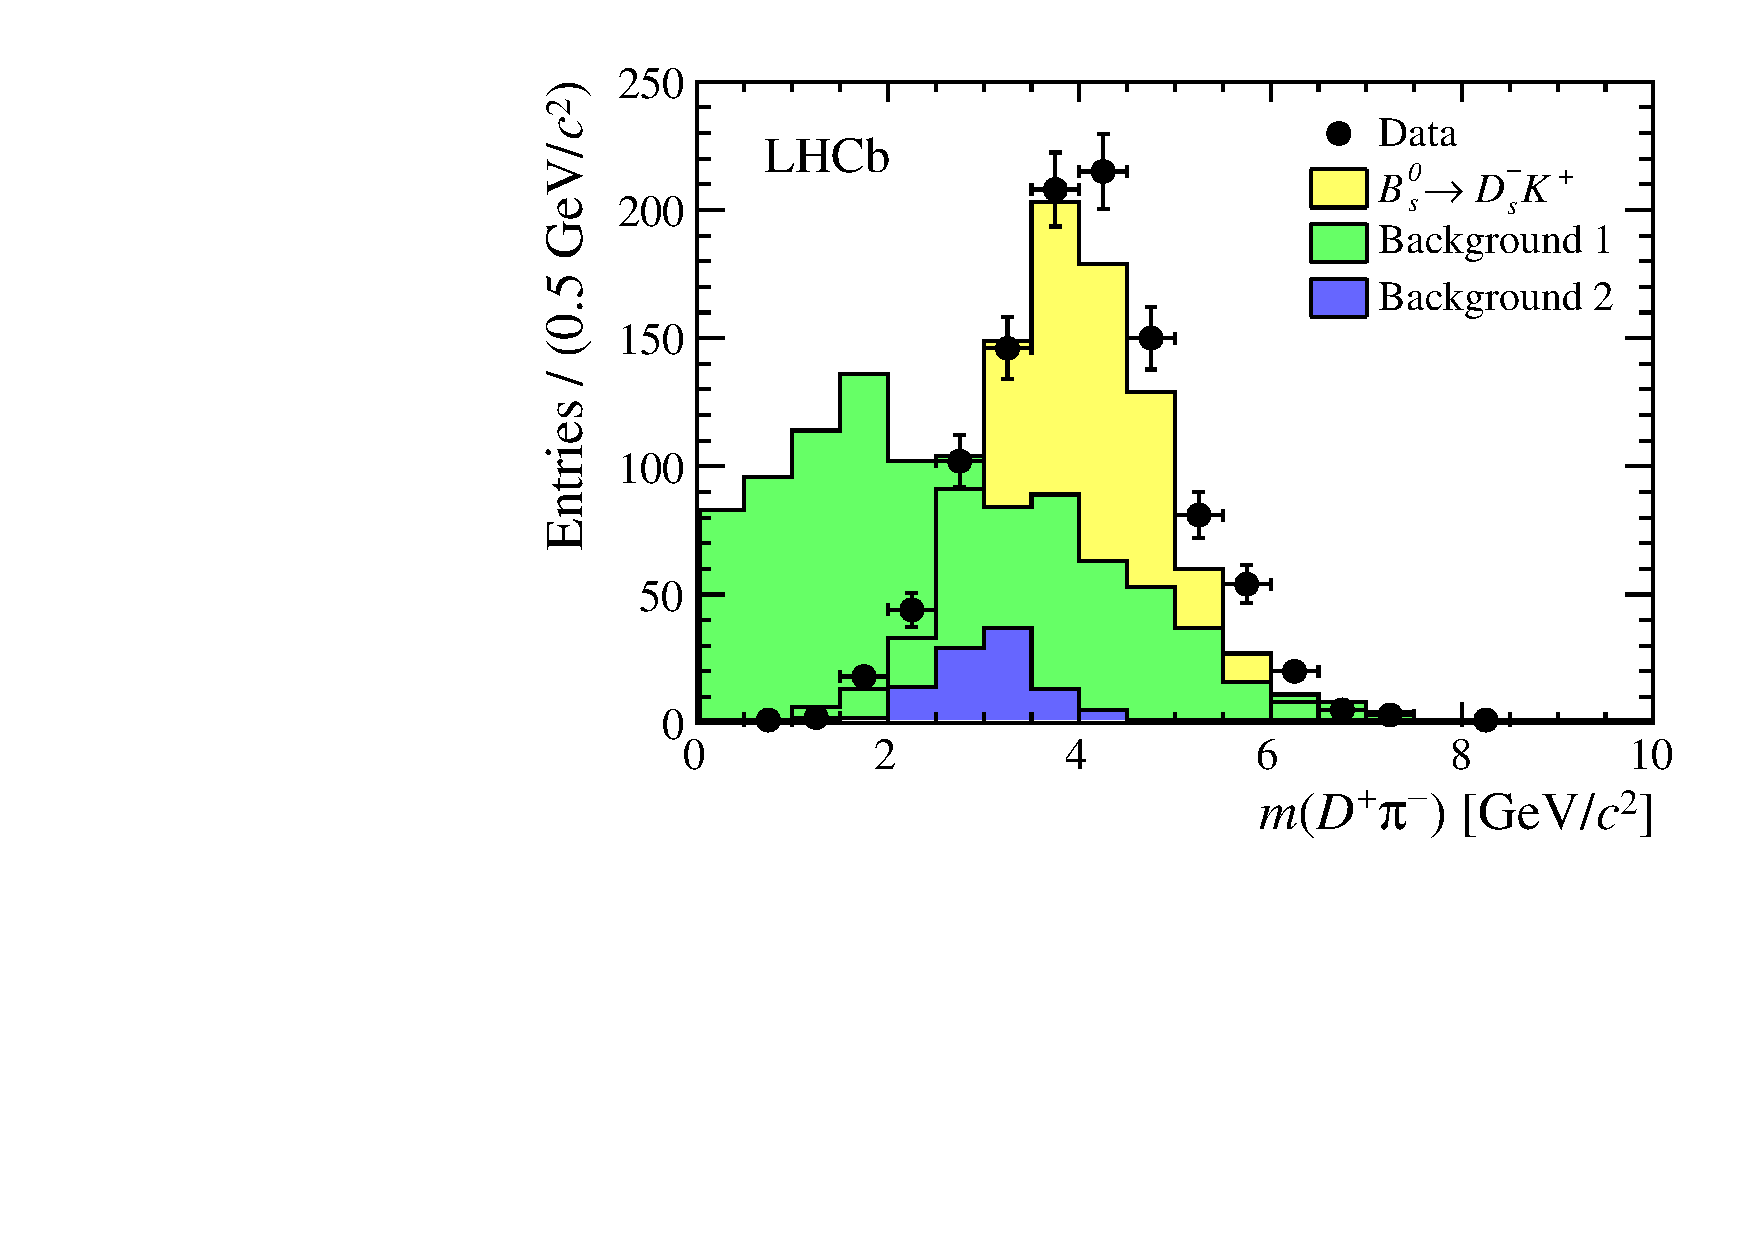
\includegraphics[width=0.49\linewidth]{Example1DPlot-python-1}\put(-32,133){(a)}
    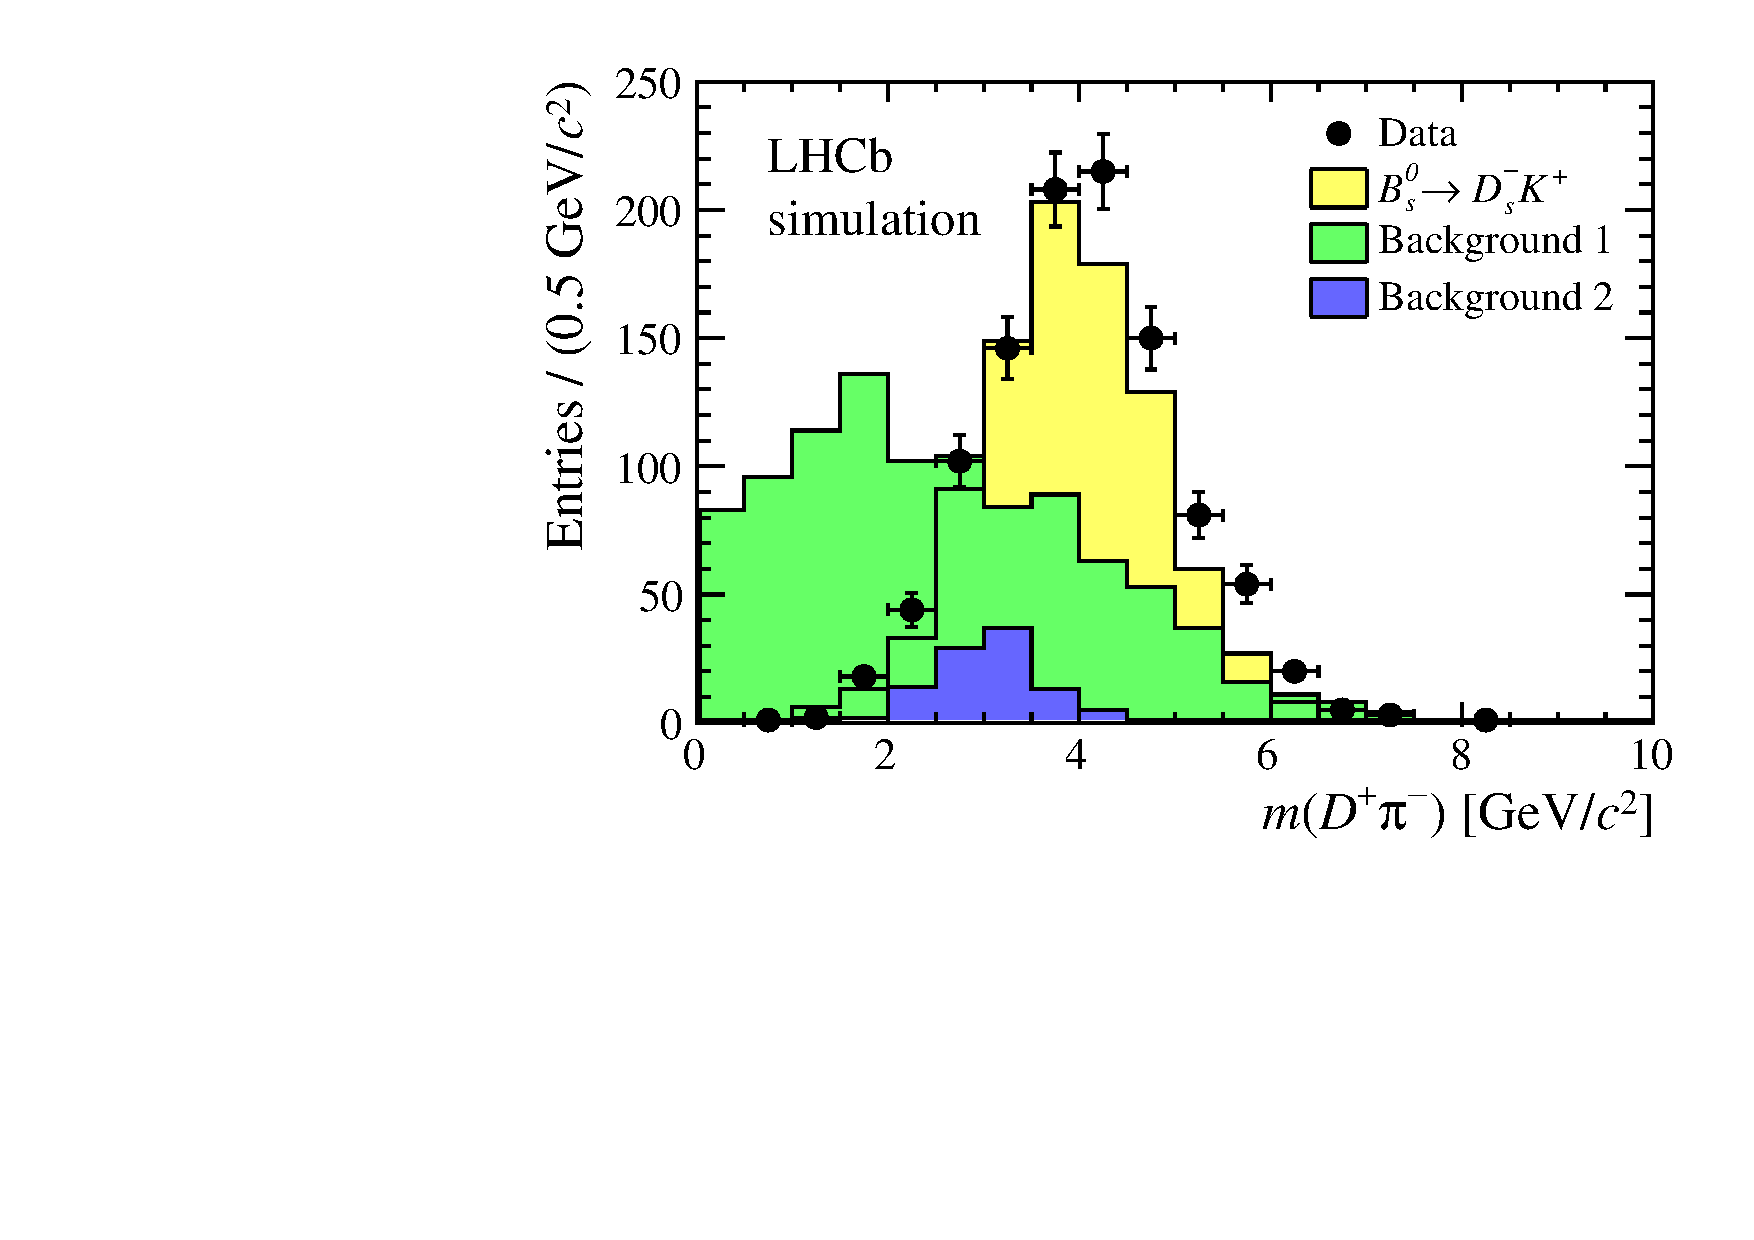
\includegraphics[width=0.49\linewidth]{Example1DPlot-python-1_sim}\put(-32,133){(b)}
    \vspace*{-1.0cm}
  \end{center}
  \caption{
    %\small %captions should be a little bit smaller than main text
    Example plots for (a) data and (b) simulation using the \lhcb style from the \urania package
    \texttt{RootTools/LHCbStyle}. The signal data is shown as points
    with the signal component as yellow (light shaded), background 1 as green
    (medium shaded) and background 2 as blue (dark shaded).}
  \label{fig:example}
\end{figure}

\begin{enumerate}

\item Figures should be legible at the size they will appear in the
  publication, with suitable line width.  Their axes should be
  labelled, and have suitable units (e.g. avoid a mass plot with
  labels in \mevcc if the region of interest covers a few \gevcc
  and all the numbers then run together).  Spurious background shading
  and boxes around text should be avoided.

\item For the $y$-axis, ``Entries'' or ``Candidates'' is approriate in case no
background subtraction has been applied. Otherwise ``Yield'' or ``Decays''
may be more appropriate. If the unit on the $y$-axis corresponds to 
the yield per bin, indicate so, for example ``Entries / ( 5\mevcc )'' or ``Entries per 5\mevcc''.


\item Fit curves should not obscure the data points, and
   data points are best (re)drawn over the fit curves.

\item Colour may be used in figures, but the distinction between
  differently coloured areas or lines should be clear also when the
  document is printed in black and white, for example through
  differently dashed lines. The \lhcb style mentioned above implements
  a colour scheme that works well but individual adjustments might be
  required.

\item Using different hatching styles helps to disinguished filled areas, 
also in black and white prints. Hatching styles 3001-3025 should be
avoided since they behave unpredictably under zooming and scaling. 
Good styles for ``falling hatched'' and ``rising hatched'' are 3345 and 3354.


\item Figures with more than one part should have the parts labelled
  (a), (b) \etc, with a corresponding description in the caption;
  alternatively they should be clearly referred to by their position,
  e.g. Fig.~1\,(left). In the caption, the labels (a), (b) \etc should
  precede their description. When referencing specific sub-figures,
  use ``see Fig. 1(a)'' or ``see Figs. 2(b)-(e)''.

\item All figures containing \lhcb data should have \lhcb written on
  them. For preliminary
  results, that should be replaced by ``LHCb preliminary''.
  Figures that only have simulated data should display ``LHCb simulation''.
  Figures that do not depend on LHCb-specific software (\eg only on \pythia)
  should not have any label.


\end{enumerate}


\section{References}
\label{sec:References}

References should be made using Bib\TeX~\cite{BibTeX}. A special style
\texttt{LHCb.bst} has been created to achieve a uniform
style. Independent of the journal the paper is submitted to, the
preprint should be created using this style. Where arXiv numbers
exist, these should be added even for published articles. In the PDF
file, hyperlinks will be created to both the arXiv and the published
version.

\begin{enumerate}

\item Citations are marked using square brackets, and the
  corresponding references should be typeset using Bib\TeX\ and the
  official \lhcb Bib\TeX\ style. An example is in
  Ref.~\cite{Sjostrand:2006za}.

\item For references with four or less authors all of the authors'
  names are listed~\cite{Majorana:1937vz}, otherwise the first author
  is given, followed by \etal. The \lhcb Bib\TeX\ style will
  take care of this.

\item The order of references should be sequential when reading the
  document. This is automatic when using Bib\TeX.

\item The titles of papers should in general be included. To remove
  them, change \texttt{\textbackslash
    setboolean\{articletitles\}\{false\}} to \texttt{true} at the top
  of this template.
  Note that the titles in \verb!LHCb-PAPER.bib! are in plain LaTex,
  in order to correspond to the actual title on the arXiv record.
  Some differences in style can thus be noticed with respect to the
  main text, for example particle names that use capital Greek letters
  are not slanted in the reference titles ($\Lambda$ vs \Lz)  

\item Whenever possible, use references from the supplied files
\verb!main.bib!, \verb!LHCb-PAPER.bib!, \verb!LHCb-CONF.bib!, and \verb!LHCB-DP.bib!.
These are kept up-to-date by the EB. If you see a mistake, do not edit these files,
but let the EB know. This way, for every update of the paper, you save
yourself the work of updating the references. Instead, you can just copy or
check in the latest versions of the \verb!.bib! files from the repository.   

\item For those references not provided by the EB, the best
  is to copy the Bib\TeX\ entry directly from
  \texttt{Inspire}. Often these need to be edited to get the 
  correct title, author names and formatting.
  For authors with multiple initials, add a space between them (change \texttt{R.G.C.} to \texttt{R. G. C.}),
  otherwise only the first initial will be taken. 
  Also, make sure to eliminate unnecessary capitalisation.
  Apart from that, the title should be respected as much as possible
  (\eg do not change particle names to PDG convention nor introduce/remove factors of $c$).
  Check that both the arXiv and the journal index are clickable
  and point to the right article.

%\item Even if the basic formatting of the Bib\TeX\ entry is taken from
%  \texttt{Inspire}, all the data should be cross checked against the
%  journal. Often there are minor changes to author initials or
%  titles. In case of a difference between the preprint and the
%  journal, the bibliographic information from the journal should be
%  used.

\item The \texttt{mciteplus}~\cite{mciteplus} package is used
  to enable multiple references to show up as a single item in the
  reference list. As an example \texttt{\textbackslash
    cite\{Mohapatra:1979ia,*Pascoli:2007qh\}} where the \texttt{*}
  indicates that the reference should be merged with the previous
  one. The result of this can be seen in
  Ref.~\cite{Mohapatra:1979ia,*Pascoli:2007qh}. Be aware that the
  \texttt{mciteplus} package should be included as the very last item
  before the \texttt{\textbackslash begin\{document\}} to work
  correctly.

\item It should be avoided to make references to public notes and
  conference reports in public documents. Exceptions can be discussed
  on a case-by-case basis with the review committee for the
  analysis. In internal reports they are of course welcome and can be
  referenced as seen in Ref.~\cite{LHCb-CONF-2011-003} using the
  \texttt{lhcbreport} category. For conference reports, omit the
  author field completely in the Bib\TeX\ record.

\item To get the typesetting and hyperlinks correct for \lhcb reports,
  the category \texttt{lhcbreport} should be used in the Bib\TeX\
  file. See Refs.~\cite{LHCb-INT-2011-047, *LHCb-ANA-2011-078,
    *CERN-THESIS-2014-057, *LHCb-PROC-2014-017, *LHCB-TALK-2014-257}
  for some examples. It can be used for \lhcb documents in the series
  \texttt{CONF}, \texttt{PAPER}, \texttt{PROC}, \texttt{THESIS},
  \texttt{LHCC}, \texttt{TDR} and internal \lhcb reports. Papers sent
  for publication, but not published yet, should be referred with
  their \texttt{arXiv} number, so the \texttt{PAPER} category should
  only be used in the rare case of a forward reference to a paper.

\item Proceedings can be used for references to items such as the
  \lhcb simulation~\cite{LHCb-PROC-2011-006}, where we do not yet have
  a published paper.

\end{enumerate}

There is a set of standard references to be used in \lhcb that are
listed in Appendix~\ref{sec:StandardReferences}.


\section{Inclusion of supplementary material}
\label{sec:Supplementary}

Three types of supplementary material should be distinguised:
\begin{itemize}
\item{A regular appendix: lengthy equations or long tables are sometimes
better put in an appendix in order not to interrupt the main flow of a paper.
Appendices will appear in the final paper, on arXiv
and on the cds record and should be considered integral
part of a paper, and are thus to be reviewed like the rest of the paper.
An example of an LHCb paper with an appendix is Ref.~\cite{LHCb-PAPER-2013-070}.
}
\item{Supplementary material for cds: plots or tables that 
would make the paper exceed the page limit or are
not appropriate to include in the paper itself,
but are desireable to be shown in public
should be added to the paper drafts in an appendix, and
removed from the paper before submitting to arXiv or the journal.
See Appendix~\ref{sec:Supplementary-App} for further instructions.
Examples are: comparison plots of the new result with older results,
plots that illustrate cross-checks.
An example of an LHCb paper with supplementary material for cds 
is Ref.~\cite{LHCb-PAPER-2013-035}.
Supplementary material for cds cannot be referenced in the paper.
Supplementary material should be included in the draft paper to be
reviewed by the collaboration.
}
\item{Supplementary material for the paper. This is usually called ``supplemental material'', which distinguishes it from supplementary material for cds only. Most journals allow
to submit files along with the paper that will not be part of the
text of the article, but will be stored on the journal server.
Examples are plain text files with numerical data corresponding to the plots
in the paper. 
The supplemental material should be cited in the paper by including a reference
which should say ``See supplemental material at [link] for [give brief description of material].''
The journal will insert a specific link for [link]. The arXiv version will usually include the supplemental material as part of the paper and so should not contain the words ``at [link]''.
Supplemental material should be included in the draft paper to be
reviewed by the collaboration.
An example of an LHCb paper with supplemental material 
is Ref.~\cite{LHCb-PAPER-2015-029}
}
\end{itemize}



\begin{acknowledgments}
\section*{Acknowledgements}

The text below are the acknowledgements as approved by the collaboration
board. Extending the acknowledgements to include individuals from outside the
collaboration who have contributed to the analysis should be approved by the
EB. The extra acknowledgements are normally placed before the standard 
acknowledgements, unless it matches better with the text of the standard 
acknowledgements to put them elsewhere. They should be included in the draft 
for the first circulation. Except in exceptional circumstances, to be approved by the
EB chair, authors of the paper should not be named in extended acknowledgements.
 
\noindent We express our gratitude to our colleagues in the CERN
accelerator departments for the excellent performance of the LHC. We
thank the technical and administrative staff at the LHCb
institutes. We acknowledge support from CERN and from the national
agencies: CAPES, CNPq, FAPERJ and FINEP (Brazil); NSFC (China);
CNRS/IN2P3 (France); BMBF, DFG and MPG (Germany); INFN (Italy); 
FOM and NWO (The Netherlands); MNiSW and NCN (Poland); MEN/IFA (Romania); 
MinES and FANO (Russia); MinECo (Spain); SNSF and SER (Switzerland); 
NASU (Ukraine); STFC (United Kingdom); NSF (USA).
We acknowledge the computing resources that are provided by CERN, IN2P3 (France), KIT and DESY (Germany), INFN (Italy), SURF (The Netherlands), PIC (Spain), GridPP (United Kingdom), RRCKI and Yandex LLC (Russia), CSCS (Switzerland), IFIN-HH (Romania), CBPF (Brazil), PL-GRID (Poland) and OSC (USA). We are indebted to the communities behind the multiple open 
source software packages on which we depend.
Individual groups or members have received support from AvH Foundation (Germany),
EPLANET, Marie Sk\l{}odowska-Curie Actions and ERC (European Union), 
Conseil G\'{e}n\'{e}ral de Haute-Savoie, Labex ENIGMASS and OCEVU, 
R\'{e}gion Auvergne (France), RFBR and Yandex LLC (Russia), GVA, XuntaGal and GENCAT (Spain), Herchel Smith Fund, The Royal Society, Royal Commission for the Exhibition of 1851 and the Leverhulme Trust (United Kingdom).

\end{acknowledgments}

% Produces the bibliography via BibTeX.
\ifthenelse{\boolean{wordcount}}%
{ \bibliographystyle{plain}
  \nobibliography{main,LHCb-PAPER,LHCb-CONF,LHCb-DP,LHCb-TDR}}
{\bibliography{main,LHCb-PAPER,LHCb-CONF,LHCb-DP,LHCb-TDR}}

% Words in appendix do not count for PRL word limit
\ifthenelse{\boolean{wordcount}}{}{%
  \clearpage
  %% $Id: appendix.tex 94782 2016-07-06 11:55:12Z michaelt $
% ===============================================================================
% Purpose: appendix to the standard template: standard symbol alises from Ulrik
% Author: Tomasz Skwarnicki
% Created on: 2009-09-24
% ===============================================================================

\clearpage

{\noindent\normalfont\bfseries\Large Appendices}

\appendix

\section{Standard References}
\label{sec:StandardReferences}
Below is a list of common references, as
well as a list of all \lhcb publications. 
As they are already in prepared bib files, they can be used as simply as
\texttt{\textbackslash cite\{Alves:2008zz\}} to get the \lhcb detector paper. 
The references are defined in the files \texttt{main.bib},  \texttt{LHCb-PAPER.bib},
\texttt{LHCb-CONF.bib}, \texttt{LHCb-DP.bib} \texttt{LHCb-TDR.bib} files, with obvious contents.
Each of these have their \texttt{LHCb-ZZZ-20XX-0YY} number as their cite code.
If you believe there is a problem with the formatting or
content of one of the entries, then get in contact with the Editorial
Board rather than just editing it in your local file,
since you are likely to need the latest version just before submiting the article.

\begin{center}
%  \begin{tabular}{llc}
  \begin{longtable}{llc}
\hline
Description & \texttt{cite} code & Reference \\
\hline
\lhcb detector & \texttt{Alves:2008zz} & \cite{Alves:2008zz} \\
%% Trigger & \texttt{LHCb-DP-2012-004} & \cite{LHCb-DP-2012-004} \\
%% RICH & \texttt{LHCb-DP-2012-003} & \cite{LHCb-DP-2012-003} \\
%% PID performance & \texttt{LHCb-PROC-2011-008} & \cite{LHCb-PROC-2011-008} \\
\lhcb simulation & \texttt{LHCb-PROC-2011-006} & \cite{LHCb-PROC-2011-006} \\
PDG 2014 & \texttt{PDG2014} & \cite{PDG2014} \\
HFAG     & \texttt{HFAG} & \cite{HFAG} \\
\pythia & \texttt{Sjostrand:2006za, *Sjostrand:2007gs} & \cite{Sjostrand:2006za, *Sjostrand:2007gs} \\
\lhcb \pythia tuning & \texttt{LHCb-PROC-2010-056} & \cite{LHCb-PROC-2010-056} \\
\geant & \texttt{Allison:2006ve, *Agostinelli:2002hh} & \cite{Allison:2006ve, *Agostinelli:2002hh} \\
\evtgen & \texttt{Lange:2001uf}  & \cite{Lange:2001uf} \\
\photos & \texttt{Golonka:2005pn}  & \cite{Golonka:2005pn} \\
\dirac & \texttt{Tsaregorodtsev:2010zz, *BelleDIRACAmazon} & \cite{Tsaregorodtsev:2010zz, *BelleDIRACAmazon}  \\
Crystal Ball function\footnote{A valid alternative for most papers where the normalisation is not critical is to use the expression``Gaussian function with a low-mass power-law tail'' or ``Gaussian function with power-law tails''. In that case, no citation is needed} & \texttt{Skwarnicki:1986xj} & \cite{Skwarnicki:1986xj} \\
Wilks' theorem & \texttt{Wilks:1938dza} & \cite{Wilks:1938dza}\\
BDT & \texttt{Breiman} & \cite{Breiman} \\
BDT training & \texttt{AdaBoost} & \cite{AdaBoost} \\
HLT2 topo & \texttt{BBDT} & \cite{BBDT} \\
DecayTreeFitter & \texttt{Hulsbergen:2005pu} & \cite{Hulsbergen:2005pu} \\
\sPlot & \texttt{Pivk:2004ty} & \cite{Pivk:2004ty} \\
Punzi's optimization & \texttt{Punzi:2003bu} & \cite{Punzi:2003bu} \\
$f_s/f_d$ & \texttt{fsfd} & \cite{fsfd} \\
\hline
\end{longtable}
%  \end{tabular}
\end{center}

\begin{center}
  %% \caption{\small
  %%   LHCb detector performance papers.
  %% }
  %% \label{tab:LHCb-DPs}
  \begin{tabular}{ll}
    \hline
    \texttt{LHCb-DP} number & Title \\
    \hline
    \texttt{LHCb-DP-2016-001}~\cite{LHCb-DP-2016-001} &
    {\small TESLA project} \\
    \texttt{LHCb-DP-2014-002}~\cite{LHCb-DP-2014-002} &
    {\small LHCb detector performance} \\
    \texttt{LHCb-DP-2014-001}~\cite{LHCb-DP-2014-001} &
    {\small Performance of the LHCb Vertex Locator} \\
    \texttt{LHCb-DP-2013-004}~\cite{LHCb-DP-2013-004} &
    {\small Performance of the LHCb calorimeters} \\
    \texttt{LHCb-DP-2013-003}~\cite{LHCb-DP-2013-003} &
    {\small Performance of the LHCb Outer Tracker} \\
    \texttt{LHCb-DP-2013-002}~\cite{LHCb-DP-2013-002} &
    {\small Measurement of the track reconstruction efficiency at LHCb} \\
    \texttt{LHCb-DP-2013-001}~\cite{LHCb-DP-2013-001} &
    {\small Performance of the muon identification at LHCb} \\
    \texttt{LHCb-DP-2012-005}~\cite{LHCb-DP-2012-005} &
    {\small Radiation damage in the LHCb Vertex Locator} \\
    \texttt{LHCb-DP-2012-004}~\cite{LHCb-DP-2012-004} &
    {\small The \lhcb trigger and its performance in 2011} \\
    \texttt{LHCb-DP-2012-003}~\cite{LHCb-DP-2012-003} &
    {\small Performance of the \lhcb RICH detector at the LHC} \\
    \texttt{LHCb-DP-2012-002}~\cite{LHCb-DP-2012-002} &
    {\small Performance of the LHCb muon system} \\
    \texttt{LHCb-DP-2012-001}~\cite{LHCb-DP-2012-001} &
    {\small Radiation hardness of the LHCb Outer Tracker} \\
    \texttt{LHCb-DP-2011-002}~\cite{LHCb-DP-2011-002} &
    {\small Simulation of machine induced background ...} \\
    \texttt{LHCb-DP-2011-001}~\cite{LHCb-DP-2011-001} &
    {\small Performance of the LHCb muon system with cosmic rays} \\
    \texttt{LHCb-DP-2010-001}~\cite{LHCb-DP-2010-001} &
    {\small First spatial alignment of the LHCb VELO ...} \\
    \hline
  \end{tabular}
\end{center}

\begin{center}
  %% \caption{\small
  %%   LHCb TDRs
  %% }
  %% \label{tab:LHCb-TDRs}
  \begin{tabular}{ll}
    \hline
    \texttt{LHCb-TDR} number & Title \\
    \hline
    \texttt{LHCb-TDR-016}~\cite{LHCb-TDR-016} &
    {\small Trigger and online upgrade} \\
    \texttt{LHCb-TDR-015}~\cite{LHCb-TDR-015} &
    {\small Tracker upgrade} \\
    \texttt{LHCb-TDR-014}~\cite{LHCb-TDR-014} &
    {\small PID upgrade} \\
    \texttt{LHCb-TDR-013}~\cite{LHCb-TDR-013} &
    {\small VELO upgrade} \\
    \texttt{LHCb-TDR-012}~\cite{LHCb-TDR-012} &
    {\small Framework TDR for the upgrade} \\
    \texttt{LHCb-TDR-011}~\cite{LHCb-TDR-011} &
    {\small Computing} \\
    \texttt{LHCb-TDR-010}~\cite{LHCb-TDR-010} &
    {\small Trigger} \\
    \texttt{LHCb-TDR-009}~\cite{LHCb-TDR-009} &
    {\small Reoptimized detector} \\
    \texttt{LHCb-TDR-008}~\cite{LHCb-TDR-008} &
    {\small Inner Tracker} \\
    \texttt{LHCb-TDR-007}~\cite{LHCb-TDR-007} &
    {\small Online, DAQ, ECS} \\
    \texttt{LHCb-TDR-006}~\cite{LHCb-TDR-006} &
    {\small Outer Tracker} \\
    \texttt{LHCb-TDR-005}~\cite{LHCb-TDR-005} &
    {\small VELO} \\
    \texttt{LHCb-TDR-004}~\cite{LHCb-TDR-004} &
    {\small Muon system} \\
    \texttt{LHCb-TDR-003}~\cite{LHCb-TDR-003} &
    {\small RICH} \\
    \texttt{LHCb-TDR-002}~\cite{LHCb-TDR-002} &
    {\small Calorimeters} \\
    \texttt{LHCb-TDR-001}~\cite{LHCb-TDR-001} &
    {\small Magnet} \\
    \hline
  \end{tabular}
\end{center}

\begin{center}
%  \begin{tabular}{l|l}
\begin{longtable}{ll}
\caption{\small
  LHCb-PAPERs (which have their identifier as their cite code).  
  Note that LHCb-PAPER-2011-039 does not exist.
}
\label{tab:LHCb-PAPERs}
\endfirsthead
\multicolumn{2}{c}{ -- continued from previous page.}
\endhead
\endfoot
\endlastfoot
\hline
& % \texttt{LHCb-PAPER-2016-030}~\cite{LHCb-PAPER-2016-030} & 
\texttt{LHCb-PAPER-2016-029}~\cite{LHCb-PAPER-2016-029} \\
\texttt{LHCb-PAPER-2016-028}~\cite{LHCb-PAPER-2016-028} & 
\texttt{LHCb-PAPER-2016-027}~\cite{LHCb-PAPER-2016-027} \\
\texttt{LHCb-PAPER-2016-026}~\cite{LHCb-PAPER-2016-026} &
\texttt{LHCb-PAPER-2016-025}~\cite{LHCb-PAPER-2016-025} \\
\texttt{LHCb-PAPER-2016-024}~\cite{LHCb-PAPER-2016-024} &
\texttt{LHCb-PAPER-2016-023}~\cite{LHCb-PAPER-2016-023} \\
\texttt{LHCb-PAPER-2016-022}~\cite{LHCb-PAPER-2016-022} &
\texttt{LHCb-PAPER-2016-021}~\cite{LHCb-PAPER-2016-021} \\
\texttt{LHCb-PAPER-2016-020}~\cite{LHCb-PAPER-2016-020} &
\texttt{LHCb-PAPER-2016-019}~\cite{LHCb-PAPER-2016-019} \\
\texttt{LHCb-PAPER-2016-018}~\cite{LHCb-PAPER-2016-018} &
\texttt{LHCb-PAPER-2016-017}~\cite{LHCb-PAPER-2016-017} \\
\texttt{LHCb-PAPER-2016-016}~\cite{LHCb-PAPER-2016-016} &
\texttt{LHCb-PAPER-2016-015}~\cite{LHCb-PAPER-2016-015} \\
\texttt{LHCb-PAPER-2016-014}~\cite{LHCb-PAPER-2016-014} &
\texttt{LHCb-PAPER-2016-013}~\cite{LHCb-PAPER-2016-013} \\
\texttt{LHCb-PAPER-2016-012}~\cite{LHCb-PAPER-2016-012} &
\texttt{LHCb-PAPER-2016-011}~\cite{LHCb-PAPER-2016-011} \\
\texttt{LHCb-PAPER-2016-010}~\cite{LHCb-PAPER-2016-010} &
\texttt{LHCb-PAPER-2016-009}~\cite{LHCb-PAPER-2016-009} \\
\texttt{LHCb-PAPER-2016-008}~\cite{LHCb-PAPER-2016-008} &
\texttt{LHCb-PAPER-2016-007}~\cite{LHCb-PAPER-2016-007} \\
\texttt{LHCb-PAPER-2016-006}~\cite{LHCb-PAPER-2016-006} &
\texttt{LHCb-PAPER-2016-005}~\cite{LHCb-PAPER-2016-005} \\
\texttt{LHCb-PAPER-2016-004}~\cite{LHCb-PAPER-2016-004} &
\texttt{LHCb-PAPER-2016-003}~\cite{LHCb-PAPER-2016-003} \\
\texttt{LHCb-PAPER-2016-002}~\cite{LHCb-PAPER-2016-002} &
\texttt{LHCb-PAPER-2016-001}~\cite{LHCb-PAPER-2016-001} \\
\hline
\texttt{LHCb-PAPER-2015-060}~\cite{LHCb-PAPER-2015-060} &
\texttt{LHCb-PAPER-2015-059}~\cite{LHCb-PAPER-2015-059} \\
\texttt{LHCb-PAPER-2015-058}~\cite{LHCb-PAPER-2015-058} &
\texttt{LHCb-PAPER-2015-057}~\cite{LHCb-PAPER-2015-057} \\
\texttt{LHCb-PAPER-2015-056}~\cite{LHCb-PAPER-2015-056} &
\texttt{LHCb-PAPER-2015-055}~\cite{LHCb-PAPER-2015-055} \\
\texttt{LHCb-PAPER-2015-054}~\cite{LHCb-PAPER-2015-054} &
\texttt{LHCb-PAPER-2015-053}~\cite{LHCb-PAPER-2015-053} \\
\texttt{LHCb-PAPER-2015-052}~\cite{LHCb-PAPER-2015-052} &
\texttt{LHCb-PAPER-2015-051}~\cite{LHCb-PAPER-2015-051} \\
\texttt{LHCb-PAPER-2015-050}~\cite{LHCb-PAPER-2015-050} &
\texttt{LHCb-PAPER-2015-049}~\cite{LHCb-PAPER-2015-049} \\
\texttt{LHCb-PAPER-2015-048}~\cite{LHCb-PAPER-2015-048} &
\texttt{LHCb-PAPER-2015-047}~\cite{LHCb-PAPER-2015-047} \\
\texttt{LHCb-PAPER-2015-046}~\cite{LHCb-PAPER-2015-046} &
\texttt{LHCb-PAPER-2015-045}~\cite{LHCb-PAPER-2015-045} \\
\texttt{LHCb-PAPER-2015-044}~\cite{LHCb-PAPER-2015-044} &
\texttt{LHCb-PAPER-2015-043}~\cite{LHCb-PAPER-2015-043} \\
\texttt{LHCb-PAPER-2015-042}~\cite{LHCb-PAPER-2015-042} &
\texttt{LHCb-PAPER-2015-041}~\cite{LHCb-PAPER-2015-041} \\
\texttt{LHCb-PAPER-2015-040}~\cite{LHCb-PAPER-2015-040} &
\texttt{LHCb-PAPER-2015-039}~\cite{LHCb-PAPER-2015-039} \\
\texttt{LHCb-PAPER-2015-038}~\cite{LHCb-PAPER-2015-038} &
\texttt{LHCb-PAPER-2015-037}~\cite{LHCb-PAPER-2015-037} \\
\texttt{LHCb-PAPER-2015-036}~\cite{LHCb-PAPER-2015-036} &
\texttt{LHCb-PAPER-2015-035}~\cite{LHCb-PAPER-2015-035} \\
\texttt{LHCb-PAPER-2015-034}~\cite{LHCb-PAPER-2015-034} &
\texttt{LHCb-PAPER-2015-033}~\cite{LHCb-PAPER-2015-033} \\
\texttt{LHCb-PAPER-2015-032}~\cite{LHCb-PAPER-2015-032} &
\texttt{LHCb-PAPER-2015-031}~\cite{LHCb-PAPER-2015-031} \\
\texttt{LHCb-PAPER-2015-030}~\cite{LHCb-PAPER-2015-030} &
\texttt{LHCb-PAPER-2015-029}~\cite{LHCb-PAPER-2015-029} \\
\texttt{LHCb-PAPER-2015-028}~\cite{LHCb-PAPER-2015-028} &
\texttt{LHCb-PAPER-2015-027}~\cite{LHCb-PAPER-2015-027} \\
\texttt{LHCb-PAPER-2015-026}~\cite{LHCb-PAPER-2015-026} &
\texttt{LHCb-PAPER-2015-025}~\cite{LHCb-PAPER-2015-025} \\
\texttt{LHCb-PAPER-2015-024}~\cite{LHCb-PAPER-2015-024} &
\texttt{LHCb-PAPER-2015-023}~\cite{LHCb-PAPER-2015-023} \\
\texttt{LHCb-PAPER-2015-022}~\cite{LHCb-PAPER-2015-022} &
\texttt{LHCb-PAPER-2015-021}~\cite{LHCb-PAPER-2015-021} \\
\texttt{LHCb-PAPER-2015-020}~\cite{LHCb-PAPER-2015-020} &
\texttt{LHCb-PAPER-2015-019}~\cite{LHCb-PAPER-2015-019} \\
\texttt{LHCb-PAPER-2015-018}~\cite{LHCb-PAPER-2015-018} &
\texttt{LHCb-PAPER-2015-017}~\cite{LHCb-PAPER-2015-017} \\
\texttt{LHCb-PAPER-2015-016}~\cite{LHCb-PAPER-2015-016} &
\texttt{LHCb-PAPER-2015-015}~\cite{LHCb-PAPER-2015-015} \\
\texttt{LHCb-PAPER-2015-014}~\cite{LHCb-PAPER-2015-014} &
\texttt{LHCb-PAPER-2015-013}~\cite{LHCb-PAPER-2015-013} \\
\texttt{LHCb-PAPER-2015-012}~\cite{LHCb-PAPER-2015-012} &
\texttt{LHCb-PAPER-2015-011}~\cite{LHCb-PAPER-2015-011} \\
\texttt{LHCb-PAPER-2015-010}~\cite{LHCb-PAPER-2015-010} &
\texttt{LHCb-PAPER-2015-009}~\cite{LHCb-PAPER-2015-009} \\
\texttt{LHCb-PAPER-2015-008}~\cite{LHCb-PAPER-2015-008} &
\texttt{LHCb-PAPER-2015-007}~\cite{LHCb-PAPER-2015-007} \\
\texttt{LHCb-PAPER-2015-006}~\cite{LHCb-PAPER-2015-006} &
\texttt{LHCb-PAPER-2015-005}~\cite{LHCb-PAPER-2015-005} \\
\texttt{LHCb-PAPER-2015-004}~\cite{LHCb-PAPER-2015-004} &
\texttt{LHCb-PAPER-2015-003}~\cite{LHCb-PAPER-2015-003} \\
\texttt{LHCb-PAPER-2015-002}~\cite{LHCb-PAPER-2015-002} &
\texttt{LHCb-PAPER-2015-001}~\cite{LHCb-PAPER-2015-001} \\
\hline
\texttt{LHCb-PAPER-2014-070}~\cite{LHCb-PAPER-2014-070} &
\texttt{LHCb-PAPER-2014-069}~\cite{LHCb-PAPER-2014-069} \\
\texttt{LHCb-PAPER-2014-068}~\cite{LHCb-PAPER-2014-068} &
\texttt{LHCb-PAPER-2014-067}~\cite{LHCb-PAPER-2014-067} \\
\texttt{LHCb-PAPER-2014-066}~\cite{LHCb-PAPER-2014-066} &
\texttt{LHCb-PAPER-2014-065}~\cite{LHCb-PAPER-2014-065} \\
\texttt{LHCb-PAPER-2014-064}~\cite{LHCb-PAPER-2014-064} &
\texttt{LHCb-PAPER-2014-063}~\cite{LHCb-PAPER-2014-063} \\
\texttt{LHCb-PAPER-2014-062}~\cite{LHCb-PAPER-2014-062} &
\texttt{LHCb-PAPER-2014-061}~\cite{LHCb-PAPER-2014-061} \\
\texttt{LHCb-PAPER-2014-060}~\cite{LHCb-PAPER-2014-060} &
\texttt{LHCb-PAPER-2014-059}~\cite{LHCb-PAPER-2014-059} \\
\texttt{LHCb-PAPER-2014-058}~\cite{LHCb-PAPER-2014-058} &
\texttt{LHCb-PAPER-2014-057}~\cite{LHCb-PAPER-2014-057} \\
\texttt{LHCb-PAPER-2014-056}~\cite{LHCb-PAPER-2014-056} &
\texttt{LHCb-PAPER-2014-055}~\cite{LHCb-PAPER-2014-055} \\
\texttt{LHCb-PAPER-2014-054}~\cite{LHCb-PAPER-2014-054} &
\texttt{LHCb-PAPER-2014-053}~\cite{LHCb-PAPER-2014-053} \\
\texttt{LHCb-PAPER-2014-052}~\cite{LHCb-PAPER-2014-052} &
\texttt{LHCb-PAPER-2014-051}~\cite{LHCb-PAPER-2014-051} \\
\texttt{LHCb-PAPER-2014-050}~\cite{LHCb-PAPER-2014-050} &
\texttt{LHCb-PAPER-2014-049}~\cite{LHCb-PAPER-2014-049} \\
\texttt{LHCb-PAPER-2014-048}~\cite{LHCb-PAPER-2014-048} &
\texttt{LHCb-PAPER-2014-047}~\cite{LHCb-PAPER-2014-047} \\
\texttt{LHCb-PAPER-2014-046}~\cite{LHCb-PAPER-2014-046} &
\texttt{LHCb-PAPER-2014-045}~\cite{LHCb-PAPER-2014-045} \\
\texttt{LHCb-PAPER-2014-044}~\cite{LHCb-PAPER-2014-044} &
\texttt{LHCb-PAPER-2014-043}~\cite{LHCb-PAPER-2014-043} \\
\texttt{LHCb-PAPER-2014-042}~\cite{LHCb-PAPER-2014-042} &
\texttt{LHCb-PAPER-2014-041}~\cite{LHCb-PAPER-2014-041} \\
\texttt{LHCb-PAPER-2014-040}~\cite{LHCb-PAPER-2014-040} &
\texttt{LHCb-PAPER-2014-039}~\cite{LHCb-PAPER-2014-039} \\
\texttt{LHCb-PAPER-2014-038}~\cite{LHCb-PAPER-2014-038} &
\texttt{LHCb-PAPER-2014-037}~\cite{LHCb-PAPER-2014-037} \\
\texttt{LHCb-PAPER-2014-036}~\cite{LHCb-PAPER-2014-036} &
\texttt{LHCb-PAPER-2014-035}~\cite{LHCb-PAPER-2014-035} \\
\texttt{LHCb-PAPER-2014-034}~\cite{LHCb-PAPER-2014-034} &
\texttt{LHCb-PAPER-2014-033}~\cite{LHCb-PAPER-2014-033} \\
\texttt{LHCb-PAPER-2014-032}~\cite{LHCb-PAPER-2014-032} &
\texttt{LHCb-PAPER-2014-031}~\cite{LHCb-PAPER-2014-031} \\
\texttt{LHCb-PAPER-2014-030}~\cite{LHCb-PAPER-2014-030} &
\texttt{LHCb-PAPER-2014-029}~\cite{LHCb-PAPER-2014-029} \\
\texttt{LHCb-PAPER-2014-028}~\cite{LHCb-PAPER-2014-028} &
\texttt{LHCb-PAPER-2014-027}~\cite{LHCb-PAPER-2014-027} \\
\texttt{LHCb-PAPER-2014-026}~\cite{LHCb-PAPER-2014-026} &
\texttt{LHCb-PAPER-2014-025}~\cite{LHCb-PAPER-2014-025} \\
\texttt{LHCb-PAPER-2014-024}~\cite{LHCb-PAPER-2014-024} &
\texttt{LHCb-PAPER-2014-023}~\cite{LHCb-PAPER-2014-023} \\
\texttt{LHCb-PAPER-2014-022}~\cite{LHCb-PAPER-2014-022} &
\texttt{LHCb-PAPER-2014-021}~\cite{LHCb-PAPER-2014-021} \\
\texttt{LHCb-PAPER-2014-020}~\cite{LHCb-PAPER-2014-020} &
\texttt{LHCb-PAPER-2014-019}~\cite{LHCb-PAPER-2014-019} \\
\texttt{LHCb-PAPER-2014-018}~\cite{LHCb-PAPER-2014-018} &
\texttt{LHCb-PAPER-2014-017}~\cite{LHCb-PAPER-2014-017} \\
\texttt{LHCb-PAPER-2014-016}~\cite{LHCb-PAPER-2014-016} &
\texttt{LHCb-PAPER-2014-015}~\cite{LHCb-PAPER-2014-015} \\
\texttt{LHCb-PAPER-2014-014}~\cite{LHCb-PAPER-2014-014} &
\texttt{LHCb-PAPER-2014-013}~\cite{LHCb-PAPER-2014-013} \\
\texttt{LHCb-PAPER-2014-012}~\cite{LHCb-PAPER-2014-012} &
\texttt{LHCb-PAPER-2014-011}~\cite{LHCb-PAPER-2014-011} \\
\texttt{LHCb-PAPER-2014-010}~\cite{LHCb-PAPER-2014-010} &
\texttt{LHCb-PAPER-2014-009}~\cite{LHCb-PAPER-2014-009} \\
\texttt{LHCb-PAPER-2014-008}~\cite{LHCb-PAPER-2014-008} &
\texttt{LHCb-PAPER-2014-007}~\cite{LHCb-PAPER-2014-007} \\
\texttt{LHCb-PAPER-2014-006}~\cite{LHCb-PAPER-2014-006} &
\texttt{LHCb-PAPER-2014-005}~\cite{LHCb-PAPER-2014-005} \\
\texttt{LHCb-PAPER-2014-004}~\cite{LHCb-PAPER-2014-004} &
\texttt{LHCb-PAPER-2014-003}~\cite{LHCb-PAPER-2014-003} \\
\texttt{LHCb-PAPER-2014-002}~\cite{LHCb-PAPER-2014-002} &
\texttt{LHCb-PAPER-2014-001}~\cite{LHCb-PAPER-2014-001} \\
\hline
\texttt{LHCb-PAPER-2013-070}~\cite{LHCb-PAPER-2013-070} &
\texttt{LHCb-PAPER-2013-069}~\cite{LHCb-PAPER-2013-069} \\
\texttt{LHCb-PAPER-2013-068}~\cite{LHCb-PAPER-2013-068} &
\texttt{LHCb-PAPER-2013-067}~\cite{LHCb-PAPER-2013-067} \\
\texttt{LHCb-PAPER-2013-066}~\cite{LHCb-PAPER-2013-066} &
\texttt{LHCb-PAPER-2013-065}~\cite{LHCb-PAPER-2013-065} \\
\texttt{LHCb-PAPER-2013-064}~\cite{LHCb-PAPER-2013-064} &
\texttt{LHCb-PAPER-2013-063}~\cite{LHCb-PAPER-2013-063} \\
\texttt{LHCb-PAPER-2013-062}~\cite{LHCb-PAPER-2013-062} &
\texttt{LHCb-PAPER-2013-061}~\cite{LHCb-PAPER-2013-061} \\
\texttt{LHCb-PAPER-2013-060}~\cite{LHCb-PAPER-2013-060} &
\texttt{LHCb-PAPER-2013-059}~\cite{LHCb-PAPER-2013-059} \\
\texttt{LHCb-PAPER-2013-058}~\cite{LHCb-PAPER-2013-058} &
\texttt{LHCb-PAPER-2013-057}~\cite{LHCb-PAPER-2013-057} \\
\texttt{LHCb-PAPER-2013-056}~\cite{LHCb-PAPER-2013-056} &
\texttt{LHCb-PAPER-2013-055}~\cite{LHCb-PAPER-2013-055} \\
\texttt{LHCb-PAPER-2013-054}~\cite{LHCb-PAPER-2013-054} &
\texttt{LHCb-PAPER-2013-053}~\cite{LHCb-PAPER-2013-053} \\
\texttt{LHCb-PAPER-2013-052}~\cite{LHCb-PAPER-2013-052} &
\texttt{LHCb-PAPER-2013-051}~\cite{LHCb-PAPER-2013-051} \\
\texttt{LHCb-PAPER-2013-050}~\cite{LHCb-PAPER-2013-050} &
\texttt{LHCb-PAPER-2013-049}~\cite{LHCb-PAPER-2013-049} \\
\texttt{LHCb-PAPER-2013-048}~\cite{LHCb-PAPER-2013-048} &
\texttt{LHCb-PAPER-2013-047}~\cite{LHCb-PAPER-2013-047} \\
\texttt{LHCb-PAPER-2013-046}~\cite{LHCb-PAPER-2013-046} &
\texttt{LHCb-PAPER-2013-045}~\cite{LHCb-PAPER-2013-045} \\
\texttt{LHCb-PAPER-2013-044}~\cite{LHCb-PAPER-2013-044} &
\texttt{LHCb-PAPER-2013-043}~\cite{LHCb-PAPER-2013-043} \\
\texttt{LHCb-PAPER-2013-042}~\cite{LHCb-PAPER-2013-042} &
\texttt{LHCb-PAPER-2013-041}~\cite{LHCb-PAPER-2013-041} \\
\texttt{LHCb-PAPER-2013-040}~\cite{LHCb-PAPER-2013-040} &
\texttt{LHCb-PAPER-2013-039}~\cite{LHCb-PAPER-2013-039} \\
\texttt{LHCb-PAPER-2013-038}~\cite{LHCb-PAPER-2013-038} &
\texttt{LHCb-PAPER-2013-037}~\cite{LHCb-PAPER-2013-037} \\
\texttt{LHCb-PAPER-2013-036}~\cite{LHCb-PAPER-2013-036} &
\texttt{LHCb-PAPER-2013-035}~\cite{LHCb-PAPER-2013-035} \\
\texttt{LHCb-PAPER-2013-034}~\cite{LHCb-PAPER-2013-034} &
\texttt{LHCb-PAPER-2013-033}~\cite{LHCb-PAPER-2013-033} \\
\texttt{LHCb-PAPER-2013-032}~\cite{LHCb-PAPER-2013-032} &
\texttt{LHCb-PAPER-2013-031}~\cite{LHCb-PAPER-2013-031} \\
\texttt{LHCb-PAPER-2013-030}~\cite{LHCb-PAPER-2013-030} &
\texttt{LHCb-PAPER-2013-029}~\cite{LHCb-PAPER-2013-029} \\
\texttt{LHCb-PAPER-2013-028}~\cite{LHCb-PAPER-2013-028} &
\texttt{LHCb-PAPER-2013-027}~\cite{LHCb-PAPER-2013-027} \\
\texttt{LHCb-PAPER-2013-026}~\cite{LHCb-PAPER-2013-026} &
\texttt{LHCb-PAPER-2013-025}~\cite{LHCb-PAPER-2013-025} \\
\texttt{LHCb-PAPER-2013-024}~\cite{LHCb-PAPER-2013-024} &
\texttt{LHCb-PAPER-2013-023}~\cite{LHCb-PAPER-2013-023} \\
\texttt{LHCb-PAPER-2013-022}~\cite{LHCb-PAPER-2013-022} &
\texttt{LHCb-PAPER-2013-021}~\cite{LHCb-PAPER-2013-021} \\
\texttt{LHCb-PAPER-2013-020}~\cite{LHCb-PAPER-2013-020} &
\texttt{LHCb-PAPER-2013-019}~\cite{LHCb-PAPER-2013-019} \\
\texttt{LHCb-PAPER-2013-018}~\cite{LHCb-PAPER-2013-018} &
\texttt{LHCb-PAPER-2013-017}~\cite{LHCb-PAPER-2013-017} \\
\texttt{LHCb-PAPER-2013-016}~\cite{LHCb-PAPER-2013-016} &
\texttt{LHCb-PAPER-2013-015}~\cite{LHCb-PAPER-2013-015} \\
\texttt{LHCb-PAPER-2013-014}~\cite{LHCb-PAPER-2013-014} &
\texttt{LHCb-PAPER-2013-013}~\cite{LHCb-PAPER-2013-013} \\
\texttt{LHCb-PAPER-2013-012}~\cite{LHCb-PAPER-2013-012} &
\texttt{LHCb-PAPER-2013-011}~\cite{LHCb-PAPER-2013-011} \\
\texttt{LHCb-PAPER-2013-010}~\cite{LHCb-PAPER-2013-010} &
\texttt{LHCb-PAPER-2013-009}~\cite{LHCb-PAPER-2013-009} \\
\texttt{LHCb-PAPER-2013-008}~\cite{LHCb-PAPER-2013-008} &
\texttt{LHCb-PAPER-2013-007}~\cite{LHCb-PAPER-2013-007} \\
\texttt{LHCb-PAPER-2013-006}~\cite{LHCb-PAPER-2013-006} &
\texttt{LHCb-PAPER-2013-005}~\cite{LHCb-PAPER-2013-005} \\
\texttt{LHCb-PAPER-2013-004}~\cite{LHCb-PAPER-2013-004} &
\texttt{LHCb-PAPER-2013-003}~\cite{LHCb-PAPER-2013-003} \\
\texttt{LHCb-PAPER-2013-002}~\cite{LHCb-PAPER-2013-002} &
\texttt{LHCb-PAPER-2013-001}~\cite{LHCb-PAPER-2013-001} \\
\hline
\texttt{LHCb-PAPER-2012-057}~\cite{LHCb-PAPER-2012-057} \\
\texttt{LHCb-PAPER-2012-056}~\cite{LHCb-PAPER-2012-056} & 
\texttt{LHCb-PAPER-2012-055}~\cite{LHCb-PAPER-2012-055} \\
\texttt{LHCb-PAPER-2012-054}~\cite{LHCb-PAPER-2012-054} & 
\texttt{LHCb-PAPER-2012-053}~\cite{LHCb-PAPER-2012-053} \\
\texttt{LHCb-PAPER-2012-052}~\cite{LHCb-PAPER-2012-052} & 
\texttt{LHCb-PAPER-2012-051}~\cite{LHCb-PAPER-2012-051} \\
\texttt{LHCb-PAPER-2012-050}~\cite{LHCb-PAPER-2012-050} & 
\texttt{LHCb-PAPER-2012-049}~\cite{LHCb-PAPER-2012-049} \\
\texttt{LHCb-PAPER-2012-048}~\cite{LHCb-PAPER-2012-048} & 
\texttt{LHCb-PAPER-2012-047}~\cite{LHCb-PAPER-2012-047} \\
\texttt{LHCb-PAPER-2012-046}~\cite{LHCb-PAPER-2012-046} & 
\texttt{LHCb-PAPER-2012-045}~\cite{LHCb-PAPER-2012-045} \\
\texttt{LHCb-PAPER-2012-044}~\cite{LHCb-PAPER-2012-044} & 
\texttt{LHCb-PAPER-2012-043}~\cite{LHCb-PAPER-2012-043} \\
\texttt{LHCb-PAPER-2012-042}~\cite{LHCb-PAPER-2012-042} & 
\texttt{LHCb-PAPER-2012-041}~\cite{LHCb-PAPER-2012-041} \\
\texttt{LHCb-PAPER-2012-040}~\cite{LHCb-PAPER-2012-040} & 
\texttt{LHCb-PAPER-2012-039}~\cite{LHCb-PAPER-2012-039} \\
\texttt{LHCb-PAPER-2012-038}~\cite{LHCb-PAPER-2012-038} & 
\texttt{LHCb-PAPER-2012-037}~\cite{LHCb-PAPER-2012-037} \\
\texttt{LHCb-PAPER-2012-036}~\cite{LHCb-PAPER-2012-036} & 
\texttt{LHCb-PAPER-2012-035}~\cite{LHCb-PAPER-2012-035} \\
\texttt{LHCb-PAPER-2012-034}~\cite{LHCb-PAPER-2012-034} & 
\texttt{LHCb-PAPER-2012-033}~\cite{LHCb-PAPER-2012-033} \\
\texttt{LHCb-PAPER-2012-032}~\cite{LHCb-PAPER-2012-032} & 
\texttt{LHCb-PAPER-2012-031}~\cite{LHCb-PAPER-2012-031} \\
\texttt{LHCb-PAPER-2012-030}~\cite{LHCb-PAPER-2012-030} & 
\texttt{LHCb-PAPER-2012-029}~\cite{LHCb-PAPER-2012-029} \\
\texttt{LHCb-PAPER-2012-028}~\cite{LHCb-PAPER-2012-028} & 
\texttt{LHCb-PAPER-2012-027}~\cite{LHCb-PAPER-2012-027} \\
\texttt{LHCb-PAPER-2012-026}~\cite{LHCb-PAPER-2012-026} & 
\texttt{LHCb-PAPER-2012-025}~\cite{LHCb-PAPER-2012-025} \\
\texttt{LHCb-PAPER-2012-024}~\cite{LHCb-PAPER-2012-024} & 
\texttt{LHCb-PAPER-2012-023}~\cite{LHCb-PAPER-2012-023} \\
\texttt{LHCb-PAPER-2012-022}~\cite{LHCb-PAPER-2012-022} & 
\texttt{LHCb-PAPER-2012-021}~\cite{LHCb-PAPER-2012-021} \\
\texttt{LHCb-PAPER-2012-020}~\cite{LHCb-PAPER-2012-020} & 
\texttt{LHCb-PAPER-2012-019}~\cite{LHCb-PAPER-2012-019} \\
\texttt{LHCb-PAPER-2012-018}~\cite{LHCb-PAPER-2012-018} & 
\texttt{LHCb-PAPER-2012-017}~\cite{LHCb-PAPER-2012-017} \\
\texttt{LHCb-PAPER-2012-016}~\cite{LHCb-PAPER-2012-016} & 
\texttt{LHCb-PAPER-2012-015}~\cite{LHCb-PAPER-2012-015} \\
\texttt{LHCb-PAPER-2012-014}~\cite{LHCb-PAPER-2012-014} & 
\texttt{LHCb-PAPER-2012-013}~\cite{LHCb-PAPER-2012-013} \\
\texttt{LHCb-PAPER-2012-012}~\cite{LHCb-PAPER-2012-012} & 
\texttt{LHCb-PAPER-2012-011}~\cite{LHCb-PAPER-2012-011} \\
\texttt{LHCb-PAPER-2012-010}~\cite{LHCb-PAPER-2012-010} & 
\texttt{LHCb-PAPER-2012-009}~\cite{LHCb-PAPER-2012-009} \\
\texttt{LHCb-PAPER-2012-008}~\cite{LHCb-PAPER-2012-008} & 
\texttt{LHCb-PAPER-2012-007}~\cite{LHCb-PAPER-2012-007} \\
\texttt{LHCb-PAPER-2012-006}~\cite{LHCb-PAPER-2012-006} & 
\texttt{LHCb-PAPER-2012-005}~\cite{LHCb-PAPER-2012-005} \\
\texttt{LHCb-PAPER-2012-004}~\cite{LHCb-PAPER-2012-004} & 
\texttt{LHCb-PAPER-2012-003}~\cite{LHCb-PAPER-2012-003} \\
\texttt{LHCb-PAPER-2012-002}~\cite{LHCb-PAPER-2012-002} & 
\texttt{LHCb-PAPER-2012-001}~\cite{LHCb-PAPER-2012-001} \\
\hline
\texttt{LHCb-PAPER-2011-045}~\cite{LHCb-PAPER-2011-045} & 
\texttt{LHCb-PAPER-2011-044}~\cite{LHCb-PAPER-2011-044} \\
\texttt{LHCb-PAPER-2011-043}~\cite{LHCb-PAPER-2011-043} & 
\texttt{LHCb-PAPER-2011-042}~\cite{LHCb-PAPER-2011-042} \\
\texttt{LHCb-PAPER-2011-041}~\cite{LHCb-PAPER-2011-041} & 
\texttt{LHCb-PAPER-2011-040}~\cite{LHCb-PAPER-2011-040} \\
% \texttt{LHCb-PAPER-2011-039}~\cite{LHCb-PAPER-2011-039} &
\texttt{LHCb-PAPER-2011-038}~\cite{LHCb-PAPER-2011-038} &
\texttt{LHCb-PAPER-2011-037}~\cite{LHCb-PAPER-2011-037} \\
\texttt{LHCb-PAPER-2011-036}~\cite{LHCb-PAPER-2011-036} &
\texttt{LHCb-PAPER-2011-035}~\cite{LHCb-PAPER-2011-035} \\
\texttt{LHCb-PAPER-2011-034}~\cite{LHCb-PAPER-2011-034} &
\texttt{LHCb-PAPER-2011-033}~\cite{LHCb-PAPER-2011-033} \\
\texttt{LHCb-PAPER-2011-032}~\cite{LHCb-PAPER-2011-032} & 
\texttt{LHCb-PAPER-2011-031}~\cite{LHCb-PAPER-2011-031} \\
\texttt{LHCb-PAPER-2011-031}~\cite{LHCb-PAPER-2011-030} &
\texttt{LHCb-PAPER-2011-029}~\cite{LHCb-PAPER-2011-029} \\
\texttt{LHCb-PAPER-2011-028}~\cite{LHCb-PAPER-2011-028} &
\texttt{LHCb-PAPER-2011-027}~\cite{LHCb-PAPER-2011-027} \\
\texttt{LHCb-PAPER-2011-026}~\cite{LHCb-PAPER-2011-026} &
\texttt{LHCb-PAPER-2011-025}~\cite{LHCb-PAPER-2011-025} \\
\texttt{LHCb-PAPER-2011-024}~\cite{LHCb-PAPER-2011-024} &
\texttt{LHCb-PAPER-2011-023}~\cite{LHCb-PAPER-2011-023} \\
\texttt{LHCb-PAPER-2011-023}~\cite{LHCb-PAPER-2011-022} &
\texttt{LHCb-PAPER-2011-021}~\cite{LHCb-PAPER-2011-021} \\
\texttt{LHCb-PAPER-2011-020}~\cite{LHCb-PAPER-2011-020} &
\texttt{LHCb-PAPER-2011-019}~\cite{LHCb-PAPER-2011-019} \\
\texttt{LHCb-PAPER-2011-018}~\cite{LHCb-PAPER-2011-018} &
\texttt{LHCb-PAPER-2011-017}~\cite{LHCb-PAPER-2011-017} \\
\texttt{LHCb-PAPER-2011-016}~\cite{LHCb-PAPER-2011-016} &
\texttt{LHCb-PAPER-2011-015}~\cite{LHCb-PAPER-2011-015} \\
\texttt{LHCb-PAPER-2011-014}~\cite{LHCb-PAPER-2011-014} &
\texttt{LHCb-PAPER-2011-013}~\cite{LHCb-PAPER-2011-013} \\
\texttt{LHCb-PAPER-2011-012}~\cite{LHCb-PAPER-2011-012} &
\texttt{LHCb-PAPER-2011-011}~\cite{LHCb-PAPER-2011-011} \\
\texttt{LHCb-PAPER-2011-010}~\cite{LHCb-PAPER-2011-010} &
\texttt{LHCb-PAPER-2011-009}~\cite{LHCb-PAPER-2011-009} \\
\texttt{LHCb-PAPER-2011-008}~\cite{LHCb-PAPER-2011-008} &
\texttt{LHCb-PAPER-2011-007}~\cite{LHCb-PAPER-2011-007} \\
\texttt{LHCb-PAPER-2011-006}~\cite{LHCb-PAPER-2011-006} &
\texttt{LHCb-PAPER-2011-005}~\cite{LHCb-PAPER-2011-005} \\
\texttt{LHCb-PAPER-2011-004}~\cite{LHCb-PAPER-2011-004} &
\texttt{LHCb-PAPER-2011-003}~\cite{LHCb-PAPER-2011-003} \\
\texttt{LHCb-PAPER-2011-002}~\cite{LHCb-PAPER-2011-002} &
\texttt{LHCb-PAPER-2011-001}~\cite{LHCb-PAPER-2011-001} \\
\hline
\texttt{LHCb-PAPER-2010-002}~\cite{LHCb-PAPER-2010-002} &
\texttt{LHCb-PAPER-2010-001}~\cite{LHCb-PAPER-2010-001} \\
\hline
%  \end{tabular}
\end{longtable}
\end{center}

\begin{center}
%  \begin{tabular}{l|l}
\begin{longtable}{ll}
\caption{\small
  LHCb-CONFs (which have their identifier as their cite code).  
  Note that LHCb-CONF-2011-032 does not exist.
}
\label{tab:LHCb-CONFs}
\endfirsthead
\multicolumn{2}{c}{ -- continued from previous page.}
\endhead
\endfoot
\endlastfoot
\hline
& %\texttt{LHCb-CONF-2016-006}~\cite{LHCb-CONF-2016-006} &
\texttt{LHCb-CONF-2016-005}~\cite{LHCb-CONF-2016-005} \\
\texttt{LHCb-CONF-2016-004}~\cite{LHCb-CONF-2016-004} &
\texttt{LHCb-CONF-2016-003}~\cite{LHCb-CONF-2016-003} \\
\texttt{LHCb-CONF-2016-002}~\cite{LHCb-CONF-2016-002} &
\texttt{LHCb-CONF-2016-001}~\cite{LHCb-CONF-2016-001} \\
\hline
\texttt{LHCb-CONF-2015-005}~\cite{LHCb-CONF-2015-005} \\
\texttt{LHCb-CONF-2015-004}~\cite{LHCb-CONF-2015-004} &
\texttt{LHCb-CONF-2015-003}~\cite{LHCb-CONF-2015-003} \\
\texttt{LHCb-CONF-2015-002}~\cite{LHCb-CONF-2015-002} &
\texttt{LHCb-CONF-2015-001}~\cite{LHCb-CONF-2015-001} \\
\hline
\texttt{LHCb-CONF-2014-004}~\cite{LHCb-CONF-2014-004}\footnote{If you cite 
the gamma combination, always also cite the latest gamma paper as
\texttt{\textbackslash{}cite\{LHCb-PAPER-2013-020,*LHCb-CONF-2014-004\}}
(unless you cite LHCb-PAPER-2013-020 separately too).} &
\texttt{LHCb-CONF-2014-003}~\cite{LHCb-CONF-2014-003} \\
\texttt{LHCb-CONF-2014-002}~\cite{LHCb-CONF-2014-002} &
\texttt{LHCb-CONF-2014-001}~\cite{LHCb-CONF-2014-001} \\
\hline
\texttt{LHCb-CONF-2013-013}~\cite{LHCb-CONF-2013-013} \\
\texttt{LHCb-CONF-2013-012}~\cite{LHCb-CONF-2013-012} &
\texttt{LHCb-CONF-2013-011}~\cite{LHCb-CONF-2013-011} \\
\texttt{LHCb-CONF-2013-010}~\cite{LHCb-CONF-2013-010} &
\texttt{LHCb-CONF-2013-009}~\cite{LHCb-CONF-2013-009} \\
\texttt{LHCb-CONF-2013-008}~\cite{LHCb-CONF-2013-008} &
\texttt{LHCb-CONF-2013-007}~\cite{LHCb-CONF-2013-007} \\
\texttt{LHCb-CONF-2013-006}~\cite{LHCb-CONF-2013-006} &
\texttt{LHCb-CONF-2013-005}~\cite{LHCb-CONF-2013-005} \\
\texttt{LHCb-CONF-2013-004}~\cite{LHCb-CONF-2013-004} &
\texttt{LHCb-CONF-2013-003}~\cite{LHCb-CONF-2013-003} \\
\texttt{LHCb-CONF-2013-002}~\cite{LHCb-CONF-2013-002} &
\texttt{LHCb-CONF-2013-001}~\cite{LHCb-CONF-2013-001} \\
\hline
\texttt{LHCb-CONF-2012-034}~\cite{LHCb-CONF-2012-034} & 
\texttt{LHCb-CONF-2012-033}~\cite{LHCb-CONF-2012-033} \\
\texttt{LHCb-CONF-2012-032}~\cite{LHCb-CONF-2012-032} & 
\texttt{LHCb-CONF-2012-031}~\cite{LHCb-CONF-2012-031} \\
\texttt{LHCb-CONF-2012-030}~\cite{LHCb-CONF-2012-030} & 
\texttt{LHCb-CONF-2012-029}~\cite{LHCb-CONF-2012-029} \\
\texttt{LHCb-CONF-2012-028}~\cite{LHCb-CONF-2012-028} & 
\texttt{LHCb-CONF-2012-027}~\cite{LHCb-CONF-2012-027} \\
\texttt{LHCb-CONF-2012-026}~\cite{LHCb-CONF-2012-026} & 
\texttt{LHCb-CONF-2012-025}~\cite{LHCb-CONF-2012-025} \\
\texttt{LHCb-CONF-2012-024}~\cite{LHCb-CONF-2012-024} & 
\texttt{LHCb-CONF-2012-023}~\cite{LHCb-CONF-2012-023} \\
\texttt{LHCb-CONF-2012-022}~\cite{LHCb-CONF-2012-022} & 
\texttt{LHCb-CONF-2012-021}~\cite{LHCb-CONF-2012-021} \\
\texttt{LHCb-CONF-2012-020}~\cite{LHCb-CONF-2012-020} & 
\texttt{LHCb-CONF-2012-019}~\cite{LHCb-CONF-2012-019} \\
\texttt{LHCb-CONF-2012-018}~\cite{LHCb-CONF-2012-018} & 
\texttt{LHCb-CONF-2012-017}~\cite{LHCb-CONF-2012-017} \\
\texttt{LHCb-CONF-2012-016}~\cite{LHCb-CONF-2012-016} & 
\texttt{LHCb-CONF-2012-015}~\cite{LHCb-CONF-2012-015} \\
\texttt{LHCb-CONF-2012-014}~\cite{LHCb-CONF-2012-014} & 
\texttt{LHCb-CONF-2012-013}~\cite{LHCb-CONF-2012-013} \\
\texttt{LHCb-CONF-2012-012}~\cite{LHCb-CONF-2012-012} & 
\texttt{LHCb-CONF-2012-011}~\cite{LHCb-CONF-2012-011} \\
\texttt{LHCb-CONF-2012-010}~\cite{LHCb-CONF-2012-010} & 
\texttt{LHCb-CONF-2012-009}~\cite{LHCb-CONF-2012-009} \\
\texttt{LHCb-CONF-2012-008}~\cite{LHCb-CONF-2012-008} & 
\texttt{LHCb-CONF-2012-007}~\cite{LHCb-CONF-2012-007} \\
\texttt{LHCb-CONF-2012-006}~\cite{LHCb-CONF-2012-006} & 
\texttt{LHCb-CONF-2012-005}~\cite{LHCb-CONF-2012-005} \\
\texttt{LHCb-CONF-2012-004}~\cite{LHCb-CONF-2012-004} & 
\texttt{LHCb-CONF-2012-003}~\cite{LHCb-CONF-2012-003} \\
\texttt{LHCb-CONF-2012-002}~\cite{LHCb-CONF-2012-002} & 
\texttt{LHCb-CONF-2012-001}~\cite{LHCb-CONF-2012-001} \\
\hline
\texttt{LHCb-CONF-2011-062}~\cite{LHCb-CONF-2011-062} &
\texttt{LHCb-CONF-2011-061}~\cite{LHCb-CONF-2011-061} \\ 
\texttt{LHCb-CONF-2011-060}~\cite{LHCb-CONF-2011-060} &
\texttt{LHCb-CONF-2011-059}~\cite{LHCb-CONF-2011-059} \\
\texttt{LHCb-CONF-2011-058}~\cite{LHCb-CONF-2011-058} & 
\texttt{LHCb-CONF-2011-057}~\cite{LHCb-CONF-2011-057} \\
\texttt{LHCb-CONF-2011-056}~\cite{LHCb-CONF-2011-056} & 
\texttt{LHCb-CONF-2011-055}~\cite{LHCb-CONF-2011-055} \\ 
\texttt{LHCb-CONF-2011-054}~\cite{LHCb-CONF-2011-054} &
\texttt{LHCb-CONF-2011-053}~\cite{LHCb-CONF-2011-053} \\ 
\texttt{LHCb-CONF-2011-052}~\cite{LHCb-CONF-2011-052} &
\texttt{LHCb-CONF-2011-051}~\cite{LHCb-CONF-2011-051} \\ 
\texttt{LHCb-CONF-2011-050}~\cite{LHCb-CONF-2011-050} &
\texttt{LHCb-CONF-2011-049}~\cite{LHCb-CONF-2011-049} \\
\texttt{LHCb-CONF-2011-048}~\cite{LHCb-CONF-2011-048} & 
\texttt{LHCb-CONF-2011-047}~\cite{LHCb-CONF-2011-047} \\
\texttt{LHCb-CONF-2011-046}~\cite{LHCb-CONF-2011-046} & 
\texttt{LHCb-CONF-2011-045}~\cite{LHCb-CONF-2011-045} \\ 
\texttt{LHCb-CONF-2011-044}~\cite{LHCb-CONF-2011-044} &
\texttt{LHCb-CONF-2011-043}~\cite{LHCb-CONF-2011-043} \\ 
\texttt{LHCb-CONF-2011-042}~\cite{LHCb-CONF-2011-042} &
\texttt{LHCb-CONF-2011-041}~\cite{LHCb-CONF-2011-041} \\ 
\texttt{LHCb-CONF-2011-040}~\cite{LHCb-CONF-2011-040} &
\texttt{LHCb-CONF-2011-039}~\cite{LHCb-CONF-2011-039} \\
\texttt{LHCb-CONF-2011-038}~\cite{LHCb-CONF-2011-038} &
\texttt{LHCb-CONF-2011-037}~\cite{LHCb-CONF-2011-037} \\
\texttt{LHCb-CONF-2011-036}~\cite{LHCb-CONF-2011-036} &
\texttt{LHCb-CONF-2011-035}~\cite{LHCb-CONF-2011-035} \\
\texttt{LHCb-CONF-2011-034}~\cite{LHCb-CONF-2011-034} &
\texttt{LHCb-CONF-2011-033}~\cite{LHCb-CONF-2011-033} \\
%\texttt{LHCb-CONF-2011-032}~\cite{LHCb-CONF-2011-032} & 
\texttt{LHCb-CONF-2011-031}~\cite{LHCb-CONF-2011-031} \\
\texttt{LHCb-CONF-2011-030}~\cite{LHCb-CONF-2011-030} &
\texttt{LHCb-CONF-2011-029}~\cite{LHCb-CONF-2011-029} \\
\texttt{LHCb-CONF-2011-028}~\cite{LHCb-CONF-2011-028} &
\texttt{LHCb-CONF-2011-027}~\cite{LHCb-CONF-2011-027} \\
\texttt{LHCb-CONF-2011-026}~\cite{LHCb-CONF-2011-026} &
\texttt{LHCb-CONF-2011-025}~\cite{LHCb-CONF-2011-025} \\
\texttt{LHCb-CONF-2011-024}~\cite{LHCb-CONF-2011-024} &
\texttt{LHCb-CONF-2011-023}~\cite{LHCb-CONF-2011-023} \\
\texttt{LHCb-CONF-2011-023}~\cite{LHCb-CONF-2011-022} &
\texttt{LHCb-CONF-2011-021}~\cite{LHCb-CONF-2011-021} \\
\texttt{LHCb-CONF-2011-020}~\cite{LHCb-CONF-2011-020} &
\texttt{LHCb-CONF-2011-019}~\cite{LHCb-CONF-2011-019} \\
\texttt{LHCb-CONF-2011-018}~\cite{LHCb-CONF-2011-018} &
\texttt{LHCb-CONF-2011-017}~\cite{LHCb-CONF-2011-017} \\
\texttt{LHCb-CONF-2011-016}~\cite{LHCb-CONF-2011-016} &
\texttt{LHCb-CONF-2011-015}~\cite{LHCb-CONF-2011-015} \\
\texttt{LHCb-CONF-2011-014}~\cite{LHCb-CONF-2011-014} &
\texttt{LHCb-CONF-2011-013}~\cite{LHCb-CONF-2011-013} \\
\texttt{LHCb-CONF-2011-012}~\cite{LHCb-CONF-2011-012} &
\texttt{LHCb-CONF-2011-011}~\cite{LHCb-CONF-2011-011} \\
\texttt{LHCb-CONF-2011-010}~\cite{LHCb-CONF-2011-010} &
\texttt{LHCb-CONF-2011-009}~\cite{LHCb-CONF-2011-009} \\
\texttt{LHCb-CONF-2011-008}~\cite{LHCb-CONF-2011-008} &
\texttt{LHCb-CONF-2011-007}~\cite{LHCb-CONF-2011-007} \\
\texttt{LHCb-CONF-2011-006}~\cite{LHCb-CONF-2011-006} &
\texttt{LHCb-CONF-2011-005}~\cite{LHCb-CONF-2011-005} \\
\texttt{LHCb-CONF-2011-004}~\cite{LHCb-CONF-2011-004} &
\texttt{LHCb-CONF-2011-003}~\cite{LHCb-CONF-2011-003} \\
\texttt{LHCb-CONF-2011-002}~\cite{LHCb-CONF-2011-002} &
\texttt{LHCb-CONF-2011-001}~\cite{LHCb-CONF-2011-001} \\
\hline
\texttt{LHCb-CONF-2010-014}~\cite{LHCb-CONF-2010-014} &
\texttt{LHCb-CONF-2010-013}~\cite{LHCb-CONF-2010-013} \\
\texttt{LHCb-CONF-2010-012}~\cite{LHCb-CONF-2010-012} &
\texttt{LHCb-CONF-2010-011}~\cite{LHCb-CONF-2010-011} \\
\texttt{LHCb-CONF-2010-010}~\cite{LHCb-CONF-2010-010} &
\texttt{LHCb-CONF-2010-009}~\cite{LHCb-CONF-2010-009} \\
\texttt{LHCb-CONF-2010-008}~\cite{LHCb-CONF-2010-008} & \\
%\texttt{LHCb-CONF-2010-007}~\cite{LHCb-CONF-2010-007} \\
%\texttt{LHCb-CONF-2010-006}~\cite{LHCb-CONF-2010-006} &
%\texttt{LHCb-CONF-2010-005}~\cite{LHCb-CONF-2010-005} \\
%\texttt{LHCb-CONF-2010-004}~\cite{LHCb-CONF-2010-004} &
%\texttt{LHCb-CONF-2010-003}~\cite{LHCb-CONF-2010-003} \\
%\texttt{LHCb-CONF-2010-002}~\cite{LHCb-CONF-2010-002} &
%\texttt{LHCb-CONF-2010-001}~\cite{LHCb-CONF-2010-001} \\
\hline
%  \end{tabular}
\end{longtable}
\end{center}

Some \lhcb papers quoted together will look
like~\cite{LHCb-PAPER-2011-007,LHCb-PAPER-2011-006,
  LHCb-PAPER-2011-005,LHCb-PAPER-2011-004,LHCb-PAPER-2011-003}.
The combination of CMS and LHCb results on $B^0_{(s)} \to \mumu$ should be cited like~\cite{LHCb-CONF-2013-012}.

\section{Standard symbols}

As explained in Sect.~\ref{sec:typography} this appendix contains standard
typesetting of symbols, particle names, units etc.\ in \lhcb
documents. 

In the file \texttt{lhcb-symbols-def.tex}, which is included, a
large number of symbols is defined. While they can lead to quicker
typing, the main reason is to ensure a uniform notation within a
document and between different \lhcb documents. If a symbol
like \texttt{\textbackslash CP} to typeset \CP violation is available
for a unit, particle name, process or whatever, it should be used.  If
you do not agree with the notation you should ask to get the
definition in \texttt{lhcb-symbols-def.tex} changed rather than just
ignoring it.

All the main particles have been given symbols. The \B mesons are thus
named \Bp, \Bd, \Bs, and \Bc. There is no need to go into math mode to
use particle names, thus saving the typing of many \$ signs. By
default particle names are typeset in italic type to agree with the
PDG preference. To get roman particle
names you can just change 
\texttt{\textbackslash setboolean\{uprightparticles\}\{false\}}
to \texttt{true} at the top of this template.

There is a large number of units typeset that ensures the correct use
of fonts, capitals and spacing. As an example we have
$\mBs=5366.3\pm0.6\mevcc$. Note that \mum is typeset with an upright
$\upmu$, even if the particle names have slanted greek letters.

A set of useful symbols are defined for working groups. More of these
symbols can be included later. As an example in the Rare Decay group
we have several different analyses looking for a measurement of
\Cpeff7 and \Opep7.

% This is an automatically generated appendix to template.tex. 
% When included it will show all the symbols defined in lhcb-symbols-def.tex.
%
% To regenerate with the latest definitions run the script ./listsymbols

\section{List of all symbols}
\label{sec:listofsymbols}
\subsection{Experiments}
\begin{tabular*}{\linewidth}{@{\extracolsep{\fill}}l@{\extracolsep{0.5cm}}l@{\extracolsep{\fill}}l@{\extracolsep{0.5cm}}l@{\extracolsep{\fill}}l@{\extracolsep{0.5cm}}l}
\texttt{\textbackslash lhcb} & \lhcb & \texttt{\textbackslash atlas} & \atlas & \texttt{\textbackslash cms} & \cms \\
\texttt{\textbackslash alice} & \alice & \texttt{\textbackslash babar} & \babar & \texttt{\textbackslash belle} & \belle \\
\texttt{\textbackslash cleo} & \cleo & \texttt{\textbackslash cdf} & \cdf & \texttt{\textbackslash dzero} & \dzero \\
\texttt{\textbackslash aleph} & \aleph & \texttt{\textbackslash delphi} & \delphi & \texttt{\textbackslash opal} & \opal \\
\texttt{\textbackslash lthree} & \lthree & \texttt{\textbackslash sld} & \sld & \texttt{\textbackslash cern} & \cern \\
\texttt{\textbackslash lhc} & \lhc & \texttt{\textbackslash lep} & \lep & \texttt{\textbackslash tevatron} & \tevatron \\
\end{tabular*}

\subsubsection{LHCb sub-detectors and sub-systems}
\begin{tabular*}{\linewidth}{@{\extracolsep{\fill}}l@{\extracolsep{0.5cm}}l@{\extracolsep{\fill}}l@{\extracolsep{0.5cm}}l@{\extracolsep{\fill}}l@{\extracolsep{0.5cm}}l}
\texttt{\textbackslash velo} & \velo & \texttt{\textbackslash rich} & \rich & \texttt{\textbackslash richone} & \richone \\
\texttt{\textbackslash richtwo} & \richtwo & \texttt{\textbackslash ttracker} & \ttracker & \texttt{\textbackslash intr} & \intr \\
\texttt{\textbackslash st} & \st & \texttt{\textbackslash ot} & \ot & \texttt{\textbackslash spd} & \spd \\
\texttt{\textbackslash presh} & \presh & \texttt{\textbackslash ecal} & \ecal & \texttt{\textbackslash hcal} & \hcal \\
\texttt{\textbackslash MagUp} & \MagUp & \texttt{\textbackslash MagDown} & \MagDown & \texttt{\textbackslash ode} & \ode \\
\texttt{\textbackslash daq} & \daq & \texttt{\textbackslash tfc} & \tfc & \texttt{\textbackslash ecs} & \ecs \\
\texttt{\textbackslash lone} & \lone & \texttt{\textbackslash hlt} & \hlt & \texttt{\textbackslash hltone} & \hltone \\
\texttt{\textbackslash hlttwo} & \hlttwo &  \\
\end{tabular*}

\subsection{Particles}
\subsubsection{Leptons}
\begin{tabular*}{\linewidth}{@{\extracolsep{\fill}}l@{\extracolsep{0.5cm}}l@{\extracolsep{\fill}}l@{\extracolsep{0.5cm}}l@{\extracolsep{\fill}}l@{\extracolsep{0.5cm}}l}
\texttt{\textbackslash electron} & \electron & \texttt{\textbackslash en} & \en & \texttt{\textbackslash ep} & \ep \\
\texttt{\textbackslash epm} & \epm & \texttt{\textbackslash epem} & \epem & \texttt{\textbackslash muon} & \muon \\
\texttt{\textbackslash mup} & \mup & \texttt{\textbackslash mun} & \mun & \texttt{\textbackslash mumu} & \mumu \\
\texttt{\textbackslash tauon} & \tauon & \texttt{\textbackslash taup} & \taup & \texttt{\textbackslash taum} & \taum \\
\texttt{\textbackslash tautau} & \tautau & \texttt{\textbackslash lepton} & \lepton & \texttt{\textbackslash ellm} & \ellm \\
\texttt{\textbackslash ellp} & \ellp & \texttt{\textbackslash ellell} & \ellell & \texttt{\textbackslash neu} & \neu \\
\texttt{\textbackslash neub} & \neub & \texttt{\textbackslash neue} & \neue & \texttt{\textbackslash neueb} & \neueb \\
\texttt{\textbackslash neum} & \neum & \texttt{\textbackslash neumb} & \neumb & \texttt{\textbackslash neut} & \neut \\
\texttt{\textbackslash neutb} & \neutb & \texttt{\textbackslash neul} & \neul & \texttt{\textbackslash neulb} & \neulb \\
\end{tabular*}

\subsubsection{Gauge bosons and scalars}
\begin{tabular*}{\linewidth}{@{\extracolsep{\fill}}l@{\extracolsep{0.5cm}}l@{\extracolsep{\fill}}l@{\extracolsep{0.5cm}}l@{\extracolsep{\fill}}l@{\extracolsep{0.5cm}}l}
\texttt{\textbackslash g} & \g & \texttt{\textbackslash H} & \H & \texttt{\textbackslash Hp} & \Hp \\
\texttt{\textbackslash Hm} & \Hm & \texttt{\textbackslash Hpm} & \Hpm & \texttt{\textbackslash W} & \W \\
\texttt{\textbackslash Wp} & \Wp & \texttt{\textbackslash Wm} & \Wm & \texttt{\textbackslash Wpm} & \Wpm \\
\texttt{\textbackslash Z} & \Z &  \\
\end{tabular*}

\subsubsection{Quarks}
\begin{tabular*}{\linewidth}{@{\extracolsep{\fill}}l@{\extracolsep{0.5cm}}l@{\extracolsep{\fill}}l@{\extracolsep{0.5cm}}l@{\extracolsep{\fill}}l@{\extracolsep{0.5cm}}l}
\texttt{\textbackslash quark} & \quark & \texttt{\textbackslash quarkbar} & \quarkbar & \texttt{\textbackslash qqbar} & \qqbar \\
\texttt{\textbackslash uquark} & \uquark & \texttt{\textbackslash uquarkbar} & \uquarkbar & \texttt{\textbackslash uubar} & \uubar \\
\texttt{\textbackslash dquark} & \dquark & \texttt{\textbackslash dquarkbar} & \dquarkbar & \texttt{\textbackslash ddbar} & \ddbar \\
\texttt{\textbackslash squark} & \squark & \texttt{\textbackslash squarkbar} & \squarkbar & \texttt{\textbackslash ssbar} & \ssbar \\
\texttt{\textbackslash cquark} & \cquark & \texttt{\textbackslash cquarkbar} & \cquarkbar & \texttt{\textbackslash ccbar} & \ccbar \\
\texttt{\textbackslash bquark} & \bquark & \texttt{\textbackslash bquarkbar} & \bquarkbar & \texttt{\textbackslash bbbar} & \bbbar \\
\texttt{\textbackslash tquark} & \tquark & \texttt{\textbackslash tquarkbar} & \tquarkbar & \texttt{\textbackslash ttbar} & \ttbar \\
\end{tabular*}

\subsubsection{Light mesons}
\begin{tabular*}{\linewidth}{@{\extracolsep{\fill}}l@{\extracolsep{0.5cm}}l@{\extracolsep{\fill}}l@{\extracolsep{0.5cm}}l@{\extracolsep{\fill}}l@{\extracolsep{0.5cm}}l}
\texttt{\textbackslash hadron} & \hadron & \texttt{\textbackslash pion} & \pion & \texttt{\textbackslash piz} & \piz \\
\texttt{\textbackslash pizs} & \pizs & \texttt{\textbackslash pip} & \pip & \texttt{\textbackslash pim} & \pim \\
\texttt{\textbackslash pipm} & \pipm & \texttt{\textbackslash pimp} & \pimp & \texttt{\textbackslash rhomeson} & \rhomeson \\
\texttt{\textbackslash rhoz} & \rhoz & \texttt{\textbackslash rhop} & \rhop & \texttt{\textbackslash rhom} & \rhom \\
\texttt{\textbackslash rhopm} & \rhopm & \texttt{\textbackslash rhomp} & \rhomp & \texttt{\textbackslash kaon} & \kaon \\
\texttt{\textbackslash Kb} & \Kb & \texttt{\textbackslash KorKbar} & \KorKbar & \texttt{\textbackslash Kz} & \Kz \\
\texttt{\textbackslash Kzb} & \Kzb & \texttt{\textbackslash Kp} & \Kp & \texttt{\textbackslash Km} & \Km \\
\texttt{\textbackslash Kpm} & \Kpm & \texttt{\textbackslash Kmp} & \Kmp & \texttt{\textbackslash KS} & \KS \\
\texttt{\textbackslash KL} & \KL & \texttt{\textbackslash Kstarz} & \Kstarz & \texttt{\textbackslash Kstarzb} & \Kstarzb \\
\texttt{\textbackslash Kstar} & \Kstar & \texttt{\textbackslash Kstarb} & \Kstarb & \texttt{\textbackslash Kstarp} & \Kstarp \\
\texttt{\textbackslash Kstarm} & \Kstarm & \texttt{\textbackslash Kstarpm} & \Kstarpm & \texttt{\textbackslash Kstarmp} & \Kstarmp \\
\texttt{\textbackslash etaz} & \etaz & \texttt{\textbackslash etapr} & \etapr & \texttt{\textbackslash phiz} & \phiz \\
\texttt{\textbackslash omegaz} & \omegaz &  \\
\end{tabular*}

\subsubsection{Heavy mesons}
\begin{tabular*}{\linewidth}{@{\extracolsep{\fill}}l@{\extracolsep{0.5cm}}l@{\extracolsep{\fill}}l@{\extracolsep{0.5cm}}l@{\extracolsep{\fill}}l@{\extracolsep{0.5cm}}l}
\texttt{\textbackslash D} & \D & \texttt{\textbackslash Db} & \Db & \texttt{\textbackslash DorDbar} & \DorDbar \\
\texttt{\textbackslash Dz} & \Dz & \texttt{\textbackslash Dzb} & \Dzb & \texttt{\textbackslash Dp} & \Dp \\
\texttt{\textbackslash Dm} & \Dm & \texttt{\textbackslash Dpm} & \Dpm & \texttt{\textbackslash Dmp} & \Dmp \\
\texttt{\textbackslash Dstar} & \Dstar & \texttt{\textbackslash Dstarb} & \Dstarb & \texttt{\textbackslash Dstarz} & \Dstarz \\
\texttt{\textbackslash Dstarzb} & \Dstarzb & \texttt{\textbackslash Dstarp} & \Dstarp & \texttt{\textbackslash Dstarm} & \Dstarm \\
\texttt{\textbackslash Dstarpm} & \Dstarpm & \texttt{\textbackslash Dstarmp} & \Dstarmp & \texttt{\textbackslash Ds} & \Ds \\
\texttt{\textbackslash Dsp} & \Dsp & \texttt{\textbackslash Dsm} & \Dsm & \texttt{\textbackslash Dspm} & \Dspm \\
\texttt{\textbackslash Dsmp} & \Dsmp & \texttt{\textbackslash Dss} & \Dss & \texttt{\textbackslash Dssp} & \Dssp \\
\texttt{\textbackslash Dssm} & \Dssm & \texttt{\textbackslash Dsspm} & \Dsspm & \texttt{\textbackslash Dssmp} & \Dssmp \\
\texttt{\textbackslash B} & \B & \texttt{\textbackslash Bbar} & \Bbar & \texttt{\textbackslash Bb} & \Bb \\
\texttt{\textbackslash BorBbar} & \BorBbar & \texttt{\textbackslash Bz} & \Bz & \texttt{\textbackslash Bzb} & \Bzb \\
\texttt{\textbackslash Bu} & \Bu & \texttt{\textbackslash Bub} & \Bub & \texttt{\textbackslash Bp} & \Bp \\
\texttt{\textbackslash Bm} & \Bm & \texttt{\textbackslash Bpm} & \Bpm & \texttt{\textbackslash Bmp} & \Bmp \\
\texttt{\textbackslash Bd} & \Bd & \texttt{\textbackslash Bs} & \Bs & \texttt{\textbackslash Bsb} & \Bsb \\
\texttt{\textbackslash Bdb} & \Bdb & \texttt{\textbackslash Bc} & \Bc & \texttt{\textbackslash Bcp} & \Bcp \\
\texttt{\textbackslash Bcm} & \Bcm & \texttt{\textbackslash Bcpm} & \Bcpm &  \\
\end{tabular*}

\subsubsection{Onia}
\begin{tabular*}{\linewidth}{@{\extracolsep{\fill}}l@{\extracolsep{0.5cm}}l@{\extracolsep{\fill}}l@{\extracolsep{0.5cm}}l@{\extracolsep{\fill}}l@{\extracolsep{0.5cm}}l}
\texttt{\textbackslash jpsi} & \jpsi & \texttt{\textbackslash psitwos} & \psitwos & \texttt{\textbackslash psiprpr} & \psiprpr \\
\texttt{\textbackslash etac} & \etac & \texttt{\textbackslash chiczero} & \chiczero & \texttt{\textbackslash chicone} & \chicone \\
\texttt{\textbackslash chictwo} & \chictwo & \texttt{\textbackslash OneS} & \OneS & \texttt{\textbackslash TwoS} & \TwoS \\
\texttt{\textbackslash ThreeS} & \ThreeS & \texttt{\textbackslash FourS} & \FourS & \texttt{\textbackslash FiveS} & \FiveS \\
\texttt{\textbackslash chic} & \chic &  \\
\end{tabular*}

\subsubsection{Baryons}
\begin{tabular*}{\linewidth}{@{\extracolsep{\fill}}l@{\extracolsep{0.5cm}}l@{\extracolsep{\fill}}l@{\extracolsep{0.5cm}}l@{\extracolsep{\fill}}l@{\extracolsep{0.5cm}}l}
\texttt{\textbackslash proton} & \proton & \texttt{\textbackslash antiproton} & \antiproton & \texttt{\textbackslash neutron} & \neutron \\
\texttt{\textbackslash antineutron} & \antineutron & \texttt{\textbackslash Deltares} & \Deltares & \texttt{\textbackslash Deltaresbar} & \Deltaresbar \\
\texttt{\textbackslash Xires} & \Xires & \texttt{\textbackslash Xiresbar} & \Xiresbar & \texttt{\textbackslash Lz} & \Lz \\
\texttt{\textbackslash Lbar} & \Lbar & \texttt{\textbackslash LorLbar} & \LorLbar & \texttt{\textbackslash Lambdares} & \Lambdares \\
\texttt{\textbackslash Lambdaresbar} & \Lambdaresbar & \texttt{\textbackslash Sigmares} & \Sigmares & \texttt{\textbackslash Sigmaresbar} & \Sigmaresbar \\
\texttt{\textbackslash Omegares} & \Omegares & \texttt{\textbackslash Omegaresbar} & \Omegaresbar & \texttt{\textbackslash Lb} & \Lb \\
\texttt{\textbackslash Lbbar} & \Lbbar & \texttt{\textbackslash Lc} & \Lc & \texttt{\textbackslash Lcbar} & \Lcbar \\
\texttt{\textbackslash Xib} & \Xib & \texttt{\textbackslash Xibz} & \Xibz & \texttt{\textbackslash Xibm} & \Xibm \\
\texttt{\textbackslash Xibbar} & \Xibbar & \texttt{\textbackslash Xibbarz} & \Xibbarz & \texttt{\textbackslash Xibbarp} & \Xibbarp \\
\texttt{\textbackslash Xic} & \Xic & \texttt{\textbackslash Xicz} & \Xicz & \texttt{\textbackslash Xicp} & \Xicp \\
\texttt{\textbackslash Xicbar} & \Xicbar & \texttt{\textbackslash Xicbarz} & \Xicbarz & \texttt{\textbackslash Xicbarm} & \Xicbarm \\
\texttt{\textbackslash Omegac} & \Omegac & \texttt{\textbackslash Omegacbar} & \Omegacbar & \texttt{\textbackslash Omegab} & \Omegab \\
\texttt{\textbackslash Omegabbar} & \Omegabbar &  \\
\end{tabular*}

\subsection{Physics symbols}
\subsubsection{Decays}
\begin{tabular*}{\linewidth}{@{\extracolsep{\fill}}l@{\extracolsep{0.5cm}}l@{\extracolsep{\fill}}l@{\extracolsep{0.5cm}}l@{\extracolsep{\fill}}l@{\extracolsep{0.5cm}}l}
\texttt{\textbackslash BF} & \BF & \texttt{\textbackslash BRvis} & \BRvis & \texttt{\textbackslash BR} & \BR \\
\texttt{\textbackslash decay[2] \textbackslash decay\{\Pa\}\{\Pb \Pc\}} & \decay{\Pa}{\Pb \Pc} & \texttt{\textbackslash ra} & \ra & \texttt{\textbackslash to} & \to \\
\end{tabular*}

\subsubsection{Lifetimes}
\begin{tabular*}{\linewidth}{@{\extracolsep{\fill}}l@{\extracolsep{0.5cm}}l@{\extracolsep{\fill}}l@{\extracolsep{0.5cm}}l@{\extracolsep{\fill}}l@{\extracolsep{0.5cm}}l}
\texttt{\textbackslash tauBs} & \tauBs & \texttt{\textbackslash tauBd} & \tauBd & \texttt{\textbackslash tauBz} & \tauBz \\
\texttt{\textbackslash tauBu} & \tauBu & \texttt{\textbackslash tauDp} & \tauDp & \texttt{\textbackslash tauDz} & \tauDz \\
\texttt{\textbackslash tauL} & \tauL & \texttt{\textbackslash tauH} & \tauH &  \\
\end{tabular*}

\subsubsection{Masses}
\begin{tabular*}{\linewidth}{@{\extracolsep{\fill}}l@{\extracolsep{0.5cm}}l@{\extracolsep{\fill}}l@{\extracolsep{0.5cm}}l@{\extracolsep{\fill}}l@{\extracolsep{0.5cm}}l}
\texttt{\textbackslash mBd} & \mBd & \texttt{\textbackslash mBp} & \mBp & \texttt{\textbackslash mBs} & \mBs \\
\texttt{\textbackslash mBc} & \mBc & \texttt{\textbackslash mLb} & \mLb &  \\
\end{tabular*}

\subsubsection{EW theory, groups}
\begin{tabular*}{\linewidth}{@{\extracolsep{\fill}}l@{\extracolsep{0.5cm}}l@{\extracolsep{\fill}}l@{\extracolsep{0.5cm}}l@{\extracolsep{\fill}}l@{\extracolsep{0.5cm}}l}
\texttt{\textbackslash grpsuthree} & \grpsuthree & \texttt{\textbackslash grpsutw} & \grpsutw & \texttt{\textbackslash grpuone} & \grpuone \\
\texttt{\textbackslash ssqtw} & \ssqtw & \texttt{\textbackslash csqtw} & \csqtw & \texttt{\textbackslash stw} & \stw \\
\texttt{\textbackslash ctw} & \ctw & \texttt{\textbackslash ssqtwef} & \ssqtwef & \texttt{\textbackslash csqtwef} & \csqtwef \\
\texttt{\textbackslash stwef} & \stwef & \texttt{\textbackslash ctwef} & \ctwef & \texttt{\textbackslash gv} & \gv \\
\texttt{\textbackslash ga} & \ga & \texttt{\textbackslash order} & \order & \texttt{\textbackslash ordalph} & \ordalph \\
\texttt{\textbackslash ordalsq} & \ordalsq & \texttt{\textbackslash ordalcb} & \ordalcb &  \\
\end{tabular*}

\subsubsection{QCD parameters}
\begin{tabular*}{\linewidth}{@{\extracolsep{\fill}}l@{\extracolsep{0.5cm}}l@{\extracolsep{\fill}}l@{\extracolsep{0.5cm}}l@{\extracolsep{\fill}}l@{\extracolsep{0.5cm}}l}
\texttt{\textbackslash as} & \as & \texttt{\textbackslash MSb} & \MSb & \texttt{\textbackslash lqcd} & \lqcd \\
\texttt{\textbackslash qsq} & \qsq &  \\
\end{tabular*}

\subsubsection{CKM, CP violation}
\begin{tabular*}{\linewidth}{@{\extracolsep{\fill}}l@{\extracolsep{0.5cm}}l@{\extracolsep{\fill}}l@{\extracolsep{0.5cm}}l@{\extracolsep{\fill}}l@{\extracolsep{0.5cm}}l}
\texttt{\textbackslash eps} & \eps & \texttt{\textbackslash epsK} & \epsK & \texttt{\textbackslash epsB} & \epsB \\
\texttt{\textbackslash epsp} & \epsp & \texttt{\textbackslash CP} & \CP & \texttt{\textbackslash CPT} & \CPT \\
\texttt{\textbackslash rhobar} & \rhobar & \texttt{\textbackslash etabar} & \etabar & \texttt{\textbackslash Vud} & \Vud \\
\texttt{\textbackslash Vcd} & \Vcd & \texttt{\textbackslash Vtd} & \Vtd & \texttt{\textbackslash Vus} & \Vus \\
\texttt{\textbackslash Vcs} & \Vcs & \texttt{\textbackslash Vts} & \Vts & \texttt{\textbackslash Vub} & \Vub \\
\texttt{\textbackslash Vcb} & \Vcb & \texttt{\textbackslash Vtb} & \Vtb & \texttt{\textbackslash Vuds} & \Vuds \\
\texttt{\textbackslash Vcds} & \Vcds & \texttt{\textbackslash Vtds} & \Vtds & \texttt{\textbackslash Vuss} & \Vuss \\
\texttt{\textbackslash Vcss} & \Vcss & \texttt{\textbackslash Vtss} & \Vtss & \texttt{\textbackslash Vubs} & \Vubs \\
\texttt{\textbackslash Vcbs} & \Vcbs & \texttt{\textbackslash Vtbs} & \Vtbs &  \\
\end{tabular*}

\subsubsection{Oscillations}
\begin{tabular*}{\linewidth}{@{\extracolsep{\fill}}l@{\extracolsep{0.5cm}}l@{\extracolsep{\fill}}l@{\extracolsep{0.5cm}}l@{\extracolsep{\fill}}l@{\extracolsep{0.5cm}}l}
\texttt{\textbackslash dm} & \dm & \texttt{\textbackslash dms} & \dms & \texttt{\textbackslash dmd} & \dmd \\
\texttt{\textbackslash DG} & \DG & \texttt{\textbackslash DGs} & \DGs & \texttt{\textbackslash DGd} & \DGd \\
\texttt{\textbackslash Gs} & \Gs & \texttt{\textbackslash Gd} & \Gd & \texttt{\textbackslash MBq} & \MBq \\
\texttt{\textbackslash DGq} & \DGq & \texttt{\textbackslash Gq} & \Gq & \texttt{\textbackslash dmq} & \dmq \\
\texttt{\textbackslash GL} & \GL & \texttt{\textbackslash GH} & \GH & \texttt{\textbackslash DGsGs} & \DGsGs \\
\texttt{\textbackslash Delm} & \Delm & \texttt{\textbackslash ACP} & \ACP & \texttt{\textbackslash Adir} & \Adir \\
\texttt{\textbackslash Amix} & \Amix & \texttt{\textbackslash ADelta} & \ADelta & \texttt{\textbackslash phid} & \phid \\
\texttt{\textbackslash sinphid} & \sinphid & \texttt{\textbackslash phis} & \phis & \texttt{\textbackslash betas} & \betas \\
\texttt{\textbackslash sbetas} & \sbetas & \texttt{\textbackslash stbetas} & \stbetas & \texttt{\textbackslash stphis} & \stphis \\
\texttt{\textbackslash sinphis} & \sinphis &  \\
\end{tabular*}

\subsubsection{Tagging}
\begin{tabular*}{\linewidth}{@{\extracolsep{\fill}}l@{\extracolsep{0.5cm}}l@{\extracolsep{\fill}}l@{\extracolsep{0.5cm}}l@{\extracolsep{\fill}}l@{\extracolsep{0.5cm}}l}
\texttt{\textbackslash edet} & \edet & \texttt{\textbackslash erec} & \erec & \texttt{\textbackslash esel} & \esel \\
\texttt{\textbackslash etrg} & \etrg & \texttt{\textbackslash etot} & \etot & \texttt{\textbackslash mistag} & \mistag \\
\texttt{\textbackslash wcomb} & \wcomb & \texttt{\textbackslash etag} & \etag & \texttt{\textbackslash etagcomb} & \etagcomb \\
\texttt{\textbackslash effeff} & \effeff & \texttt{\textbackslash effeffcomb} & \effeffcomb & \texttt{\textbackslash efftag} & \efftag \\
\texttt{\textbackslash effD} & \effD & \texttt{\textbackslash etagprompt} & \etagprompt & \texttt{\textbackslash etagLL} & \etagLL \\
\end{tabular*}

\subsubsection{Key decay channels}
\begin{tabular*}{\linewidth}{@{\extracolsep{\fill}}l@{\extracolsep{0.5cm}}l@{\extracolsep{\fill}}l@{\extracolsep{0.5cm}}l@{\extracolsep{\fill}}l@{\extracolsep{0.5cm}}l}
\texttt{\textbackslash BdToKstmm} & \BdToKstmm & \texttt{\textbackslash BdbToKstmm} & \BdbToKstmm & \texttt{\textbackslash BsToJPsiPhi} & \BsToJPsiPhi \\
\texttt{\textbackslash BdToJPsiKst} & \BdToJPsiKst & \texttt{\textbackslash BdbToJPsiKst} & \BdbToJPsiKst & \texttt{\textbackslash BsPhiGam} & \BsPhiGam \\
\texttt{\textbackslash BdKstGam} & \BdKstGam & \texttt{\textbackslash BTohh} & \BTohh & \texttt{\textbackslash BdTopipi} & \BdTopipi \\
\texttt{\textbackslash BdToKpi} & \BdToKpi & \texttt{\textbackslash BsToKK} & \BsToKK & \texttt{\textbackslash BsTopiK} & \BsTopiK \\
\end{tabular*}

\subsubsection{Rare decays}
\begin{tabular*}{\linewidth}{@{\extracolsep{\fill}}l@{\extracolsep{0.5cm}}l@{\extracolsep{\fill}}l@{\extracolsep{0.5cm}}l@{\extracolsep{\fill}}l@{\extracolsep{0.5cm}}l}
\texttt{\textbackslash BdKstee} & \BdKstee & \texttt{\textbackslash BdbKstee} & \BdbKstee & \texttt{\textbackslash bsll} & \bsll \\
\texttt{\textbackslash AFB} & \AFB & \texttt{\textbackslash FL} & \FL & \texttt{\textbackslash AT\#1 \textbackslash AT2} & \AT2 \\
\texttt{\textbackslash btosgam} & \btosgam & \texttt{\textbackslash btodgam} & \btodgam & \texttt{\textbackslash Bsmm} & \Bsmm \\
\texttt{\textbackslash Bdmm} & \Bdmm & \texttt{\textbackslash ctl} & \ctl & \texttt{\textbackslash ctk} & \ctk \\
\end{tabular*}

\subsubsection{Wilson coefficients and operators}
\begin{tabular*}{\linewidth}{@{\extracolsep{\fill}}l@{\extracolsep{0.5cm}}l@{\extracolsep{\fill}}l@{\extracolsep{0.5cm}}l@{\extracolsep{\fill}}l@{\extracolsep{0.5cm}}l}
\texttt{\textbackslash C\#1 \textbackslash C9} & \C9 & \texttt{\textbackslash Cp\#1 \textbackslash Cp7} & \Cp7 & \texttt{\textbackslash Ceff\#1 \textbackslash Ceff9  } & \Ceff9   \\
\texttt{\textbackslash Cpeff\#1 \textbackslash Cpeff7} & \Cpeff7 & \texttt{\textbackslash Ope\#1 \textbackslash Ope2} & \Ope2 & \texttt{\textbackslash Opep\#1 \textbackslash Opep7} & \Opep7 \\
\end{tabular*}

\subsubsection{Charm}
\begin{tabular*}{\linewidth}{@{\extracolsep{\fill}}l@{\extracolsep{0.5cm}}l@{\extracolsep{\fill}}l@{\extracolsep{0.5cm}}l@{\extracolsep{\fill}}l@{\extracolsep{0.5cm}}l}
\texttt{\textbackslash xprime} & \xprime & \texttt{\textbackslash yprime} & \yprime & \texttt{\textbackslash ycp} & \ycp \\
\texttt{\textbackslash agamma} & \agamma & \texttt{\textbackslash dkpicf} & \dkpicf &  \\
\end{tabular*}

\subsubsection{QM}
\begin{tabular*}{\linewidth}{@{\extracolsep{\fill}}l@{\extracolsep{0.5cm}}l@{\extracolsep{\fill}}l@{\extracolsep{0.5cm}}l@{\extracolsep{\fill}}l@{\extracolsep{0.5cm}}l}
\texttt{\textbackslash bra[1] \textbackslash bra\{a\}} & \bra{a} & \texttt{\textbackslash ket[1] \textbackslash ket\{b\}} & \ket{b} & \texttt{\textbackslash braket[2] \textbackslash braket\{a\}\{b\}} & \braket{a}{b} \\
\end{tabular*}

\subsection{Units}
\begin{tabular*}{\linewidth}{@{\extracolsep{\fill}}l@{\extracolsep{0.5cm}}l@{\extracolsep{\fill}}l@{\extracolsep{0.5cm}}l@{\extracolsep{\fill}}l@{\extracolsep{0.5cm}}l}
\texttt{\textbackslash unit[1] \textbackslash unit\{kg\}} & \unit{kg} &  \\
\end{tabular*}

\subsubsection{Energy and momentum}
\begin{tabular*}{\linewidth}{@{\extracolsep{\fill}}l@{\extracolsep{0.5cm}}l@{\extracolsep{\fill}}l@{\extracolsep{0.5cm}}l@{\extracolsep{\fill}}l@{\extracolsep{0.5cm}}l}
\texttt{\textbackslash tev} & \tev & \texttt{\textbackslash gev} & \gev & \texttt{\textbackslash mev} & \mev \\
\texttt{\textbackslash kev} & \kev & \texttt{\textbackslash ev} & \ev & \texttt{\textbackslash gevc} & \gevc \\
\texttt{\textbackslash mevc} & \mevc & \texttt{\textbackslash gevcc} & \gevcc & \texttt{\textbackslash gevgevcccc} & \gevgevcccc \\
\texttt{\textbackslash mevcc} & \mevcc &  \\
\end{tabular*}

\subsubsection{Distance and area}
\begin{tabular*}{\linewidth}{@{\extracolsep{\fill}}l@{\extracolsep{0.5cm}}l@{\extracolsep{\fill}}l@{\extracolsep{0.5cm}}l@{\extracolsep{\fill}}l@{\extracolsep{0.5cm}}l}
\texttt{\textbackslash km} & \km & \texttt{\textbackslash m} & \m & \texttt{\textbackslash ma} & \ma \\
\texttt{\textbackslash cm} & \cm & \texttt{\textbackslash cma} & \cma & \texttt{\textbackslash mm} & \mm \\
\texttt{\textbackslash mma} & \mma & \texttt{\textbackslash mum} & \mum & \texttt{\textbackslash muma} & \muma \\
\texttt{\textbackslash nm} & \nm & \texttt{\textbackslash fm} & \fm & \texttt{\textbackslash barn} & \barn \\
\texttt{\textbackslash mbarn} & \mbarn & \texttt{\textbackslash mub} & \mub & \texttt{\textbackslash nb} & \nb \\
\texttt{\textbackslash invnb} & \invnb & \texttt{\textbackslash pb} & \pb & \texttt{\textbackslash invpb} & \invpb \\
\texttt{\textbackslash fb} & \fb & \texttt{\textbackslash invfb} & \invfb & \texttt{\textbackslash ab} & \ab \\
\texttt{\textbackslash invab} & \invab &  \\
\end{tabular*}

\subsubsection{Time }
\begin{tabular*}{\linewidth}{@{\extracolsep{\fill}}l@{\extracolsep{0.5cm}}l@{\extracolsep{\fill}}l@{\extracolsep{0.5cm}}l@{\extracolsep{\fill}}l@{\extracolsep{0.5cm}}l}
\texttt{\textbackslash sec} & \sec & \texttt{\textbackslash ms} & \ms & \texttt{\textbackslash mus} & \mus \\
\texttt{\textbackslash ns} & \ns & \texttt{\textbackslash ps} & \ps & \texttt{\textbackslash fs} & \fs \\
\texttt{\textbackslash mhz} & \mhz & \texttt{\textbackslash khz} & \khz & \texttt{\textbackslash hz} & \hz \\
\texttt{\textbackslash invps} & \invps & \texttt{\textbackslash invns} & \invns & \texttt{\textbackslash yr} & \yr \\
\texttt{\textbackslash hr} & \hr &  \\
\end{tabular*}

\subsubsection{Temperature}
\begin{tabular*}{\linewidth}{@{\extracolsep{\fill}}l@{\extracolsep{0.5cm}}l@{\extracolsep{\fill}}l@{\extracolsep{0.5cm}}l@{\extracolsep{\fill}}l@{\extracolsep{0.5cm}}l}
\texttt{\textbackslash degc} & \degc & \texttt{\textbackslash degk} & \degk &  \\
\end{tabular*}

\subsubsection{Material lengths, radiation}
\begin{tabular*}{\linewidth}{@{\extracolsep{\fill}}l@{\extracolsep{0.5cm}}l@{\extracolsep{\fill}}l@{\extracolsep{0.5cm}}l@{\extracolsep{\fill}}l@{\extracolsep{0.5cm}}l}
\texttt{\textbackslash Xrad} & \Xrad & \texttt{\textbackslash NIL} & \NIL & \texttt{\textbackslash mip} & \mip \\
\texttt{\textbackslash neutroneq} & \neutroneq & \texttt{\textbackslash neqcmcm} & \neqcmcm & \texttt{\textbackslash kRad} & \kRad \\
\texttt{\textbackslash MRad} & \MRad & \texttt{\textbackslash ci} & \ci & \texttt{\textbackslash mci} & \mci \\
\end{tabular*}

\subsubsection{Uncertainties}
\begin{tabular*}{\linewidth}{@{\extracolsep{\fill}}l@{\extracolsep{0.5cm}}l@{\extracolsep{\fill}}l@{\extracolsep{0.5cm}}l@{\extracolsep{\fill}}l@{\extracolsep{0.5cm}}l}
\texttt{\textbackslash sx} & \sx & \texttt{\textbackslash sy} & \sy & \texttt{\textbackslash sz} & \sz \\
\texttt{\textbackslash stat} & \stat & \texttt{\textbackslash syst} & \syst &  \\
\end{tabular*}

\subsubsection{Maths}
\begin{tabular*}{\linewidth}{@{\extracolsep{\fill}}l@{\extracolsep{0.5cm}}l@{\extracolsep{\fill}}l@{\extracolsep{0.5cm}}l@{\extracolsep{\fill}}l@{\extracolsep{0.5cm}}l}
\texttt{\textbackslash order} & \order & \texttt{\textbackslash chisq} & \chisq & \texttt{\textbackslash chisqndf} & \chisqndf \\
\texttt{\textbackslash chisqip} & \chisqip & \texttt{\textbackslash chisqvs} & \chisqvs & \texttt{\textbackslash chisqvtx} & \chisqvtx \\
\texttt{\textbackslash chisqvtxndf} & \chisqvtxndf & \texttt{\textbackslash deriv} & \deriv & \texttt{\textbackslash gsim} & \gsim \\
\texttt{\textbackslash lsim} & \lsim & \texttt{\textbackslash mean[1] \textbackslash mean\{x\}} & \mean{x} & \texttt{\textbackslash abs[1] \textbackslash abs\{x\}} & \abs{x} \\
\texttt{\textbackslash Real} & \Real & \texttt{\textbackslash Imag} & \Imag & \texttt{\textbackslash PDF} & \PDF \\
\texttt{\textbackslash sPlot} & \sPlot &  \\
\end{tabular*}

\subsection{Kinematics}
\subsubsection{Energy, Momenta}
\begin{tabular*}{\linewidth}{@{\extracolsep{\fill}}l@{\extracolsep{0.5cm}}l@{\extracolsep{\fill}}l@{\extracolsep{0.5cm}}l@{\extracolsep{\fill}}l@{\extracolsep{0.5cm}}l}
\texttt{\textbackslash Ebeam} & \Ebeam & \texttt{\textbackslash sqs} & \sqs & \texttt{\textbackslash ptot} & \ptot \\
\texttt{\textbackslash pt} & \pt & \texttt{\textbackslash et} & \et & \texttt{\textbackslash mt} & \mt \\
\texttt{\textbackslash dpp} & \dpp & \texttt{\textbackslash msq} & \msq & \texttt{\textbackslash dedx} & \dedx \\
\end{tabular*}

\subsubsection{PID}
\begin{tabular*}{\linewidth}{@{\extracolsep{\fill}}l@{\extracolsep{0.5cm}}l@{\extracolsep{\fill}}l@{\extracolsep{0.5cm}}l@{\extracolsep{\fill}}l@{\extracolsep{0.5cm}}l}
\texttt{\textbackslash dllkpi} & \dllkpi & \texttt{\textbackslash dllppi} & \dllppi & \texttt{\textbackslash dllepi} & \dllepi \\
\texttt{\textbackslash dllmupi} & \dllmupi &  \\
\end{tabular*}

\subsubsection{Geometry}
\begin{tabular*}{\linewidth}{@{\extracolsep{\fill}}l@{\extracolsep{0.5cm}}l@{\extracolsep{\fill}}l@{\extracolsep{0.5cm}}l@{\extracolsep{\fill}}l@{\extracolsep{0.5cm}}l}
\texttt{\textbackslash degrees} & \degrees & \texttt{\textbackslash krad} & \krad & \texttt{\textbackslash mrad} & \mrad \\
\texttt{\textbackslash rad} & \rad &  \\
\end{tabular*}

\subsubsection{Accelerator}
\begin{tabular*}{\linewidth}{@{\extracolsep{\fill}}l@{\extracolsep{0.5cm}}l@{\extracolsep{\fill}}l@{\extracolsep{0.5cm}}l@{\extracolsep{\fill}}l@{\extracolsep{0.5cm}}l}
\texttt{\textbackslash betastar} & \betastar & \texttt{\textbackslash lum} & \lum & \texttt{\textbackslash intlum[1] \textbackslash intlum\{2 \,\invfb\}} & \intlum{2 \,\invfb} \\
\end{tabular*}

\subsection{Software}
\subsubsection{Programs}
\begin{tabular*}{\linewidth}{@{\extracolsep{\fill}}l@{\extracolsep{0.5cm}}l@{\extracolsep{\fill}}l@{\extracolsep{0.5cm}}l@{\extracolsep{\fill}}l@{\extracolsep{0.5cm}}l}
\texttt{\textbackslash bcvegpy} & \bcvegpy & \texttt{\textbackslash boole} & \boole & \texttt{\textbackslash brunel} & \brunel \\
\texttt{\textbackslash davinci} & \davinci & \texttt{\textbackslash dirac} & \dirac & \texttt{\textbackslash evtgen} & \evtgen \\
\texttt{\textbackslash fewz} & \fewz & \texttt{\textbackslash fluka} & \fluka & \texttt{\textbackslash ganga} & \ganga \\
\texttt{\textbackslash gaudi} & \gaudi & \texttt{\textbackslash gauss} & \gauss & \texttt{\textbackslash geant} & \geant \\
\texttt{\textbackslash hepmc} & \hepmc & \texttt{\textbackslash herwig} & \herwig & \texttt{\textbackslash moore} & \moore \\
\texttt{\textbackslash neurobayes} & \neurobayes & \texttt{\textbackslash photos} & \photos & \texttt{\textbackslash powheg} & \powheg \\
\texttt{\textbackslash pythia} & \pythia & \texttt{\textbackslash resbos} & \resbos & \texttt{\textbackslash roofit} & \roofit \\
\texttt{\textbackslash root} & \root & \texttt{\textbackslash spice} & \spice & \texttt{\textbackslash urania} & \urania \\
\end{tabular*}

\subsubsection{Languages}
\begin{tabular*}{\linewidth}{@{\extracolsep{\fill}}l@{\extracolsep{0.5cm}}l@{\extracolsep{\fill}}l@{\extracolsep{0.5cm}}l@{\extracolsep{\fill}}l@{\extracolsep{0.5cm}}l}
\texttt{\textbackslash cpp} & \cpp & \texttt{\textbackslash ruby} & \ruby & \texttt{\textbackslash fortran} & \fortran \\
\texttt{\textbackslash svn} & \svn &  \\
\end{tabular*}

\subsubsection{Data processing}
\begin{tabular*}{\linewidth}{@{\extracolsep{\fill}}l@{\extracolsep{0.5cm}}l@{\extracolsep{\fill}}l@{\extracolsep{0.5cm}}l@{\extracolsep{\fill}}l@{\extracolsep{0.5cm}}l}
\texttt{\textbackslash kbytes} & \kbytes & \texttt{\textbackslash kbsps} & \kbsps & \texttt{\textbackslash kbits} & \kbits \\
\texttt{\textbackslash kbsps} & \kbsps & \texttt{\textbackslash mbsps} & \mbsps & \texttt{\textbackslash mbytes} & \mbytes \\
\texttt{\textbackslash mbps} & \mbps & \texttt{\textbackslash mbsps} & \mbsps & \texttt{\textbackslash gbsps} & \gbsps \\
\texttt{\textbackslash gbytes} & \gbytes & \texttt{\textbackslash gbsps} & \gbsps & \texttt{\textbackslash tbytes} & \tbytes \\
\texttt{\textbackslash tbpy} & \tbpy & \texttt{\textbackslash dst} & \dst &  \\
\end{tabular*}

\subsection{Detector related}
\subsubsection{Detector technologies}
\begin{tabular*}{\linewidth}{@{\extracolsep{\fill}}l@{\extracolsep{0.5cm}}l@{\extracolsep{\fill}}l@{\extracolsep{0.5cm}}l@{\extracolsep{\fill}}l@{\extracolsep{0.5cm}}l}
\texttt{\textbackslash nonn} & \nonn & \texttt{\textbackslash ponn} & \ponn & \texttt{\textbackslash nonp} & \nonp \\
\texttt{\textbackslash cvd} & \cvd & \texttt{\textbackslash mwpc} & \mwpc & \texttt{\textbackslash gem} & \gem \\
\end{tabular*}

\subsubsection{Detector components, electronics}
\begin{tabular*}{\linewidth}{@{\extracolsep{\fill}}l@{\extracolsep{0.5cm}}l@{\extracolsep{\fill}}l@{\extracolsep{0.5cm}}l@{\extracolsep{\fill}}l@{\extracolsep{0.5cm}}l}
\texttt{\textbackslash tell1} & \tell1 & \texttt{\textbackslash ukl1} & \ukl1 & \texttt{\textbackslash beetle} & \beetle \\
\texttt{\textbackslash otis} & \otis & \texttt{\textbackslash croc} & \croc & \texttt{\textbackslash carioca} & \carioca \\
\texttt{\textbackslash dialog} & \dialog & \texttt{\textbackslash sync} & \sync & \texttt{\textbackslash cardiac} & \cardiac \\
\texttt{\textbackslash gol} & \gol & \texttt{\textbackslash vcsel} & \vcsel & \texttt{\textbackslash ttc} & \ttc \\
\texttt{\textbackslash ttcrx} & \ttcrx & \texttt{\textbackslash hpd} & \hpd & \texttt{\textbackslash pmt} & \pmt \\
\texttt{\textbackslash specs} & \specs & \texttt{\textbackslash elmb} & \elmb & \texttt{\textbackslash fpga} & \fpga \\
\texttt{\textbackslash plc} & \plc & \texttt{\textbackslash rasnik} & \rasnik & \texttt{\textbackslash elmb} & \elmb \\
\texttt{\textbackslash can} & \can & \texttt{\textbackslash lvds} & \lvds & \texttt{\textbackslash ntc} & \ntc \\
\texttt{\textbackslash adc} & \adc & \texttt{\textbackslash led} & \led & \texttt{\textbackslash ccd} & \ccd \\
\texttt{\textbackslash hv} & \hv & \texttt{\textbackslash lv} & \lv & \texttt{\textbackslash pvss} & \pvss \\
\texttt{\textbackslash cmos} & \cmos & \texttt{\textbackslash fifo} & \fifo & \texttt{\textbackslash ccpc} & \ccpc \\
\end{tabular*}

\subsubsection{Chemical symbols}
\begin{tabular*}{\linewidth}{@{\extracolsep{\fill}}l@{\extracolsep{0.5cm}}l@{\extracolsep{\fill}}l@{\extracolsep{0.5cm}}l@{\extracolsep{\fill}}l@{\extracolsep{0.5cm}}l}
\texttt{\textbackslash cfourften} & \cfourften & \texttt{\textbackslash cffour} & \cffour & \texttt{\textbackslash cotwo} & \cotwo \\
\texttt{\textbackslash csixffouteen} & \csixffouteen & \texttt{\textbackslash mgftwo} & \mgftwo & \texttt{\textbackslash siotwo} & \siotwo \\
\end{tabular*}

\subsection{Special Text }
\begin{tabular*}{\linewidth}{@{\extracolsep{\fill}}l@{\extracolsep{0.5cm}}l@{\extracolsep{\fill}}l@{\extracolsep{0.5cm}}l@{\extracolsep{\fill}}l@{\extracolsep{0.5cm}}l}
\texttt{\textbackslash eg} & \eg & \texttt{\textbackslash ie} & \ie & \texttt{\textbackslash etal} & \etal \\
\texttt{\textbackslash etc} & \etc & \texttt{\textbackslash cf} & \cf & \texttt{\textbackslash ffp} & \ffp \\
\texttt{\textbackslash vs} & \vs &  \\
\end{tabular*}



 # this does not compile with revtex
  \appendix

  % This should be taken out in the final paper
  \clearpage

\section{Supplementary material for LHCb-PAPER-20XX-YYY}
\label{sec:Supplementary-App}

This appendix contains supplementary material that will posted
on the public cds record but will not appear in the paper.

Please leave the above sentence in your draft for first and 
second circulation and replace what follows by your actual supplementary material.
For more information about other types of supplementary material, see Section~\ref{sec:Supplementary}. Plots and tables that follow should be well described, either with captions or with additional explanatory text.


\begin{figure}[!htb]
  \begin{center}
    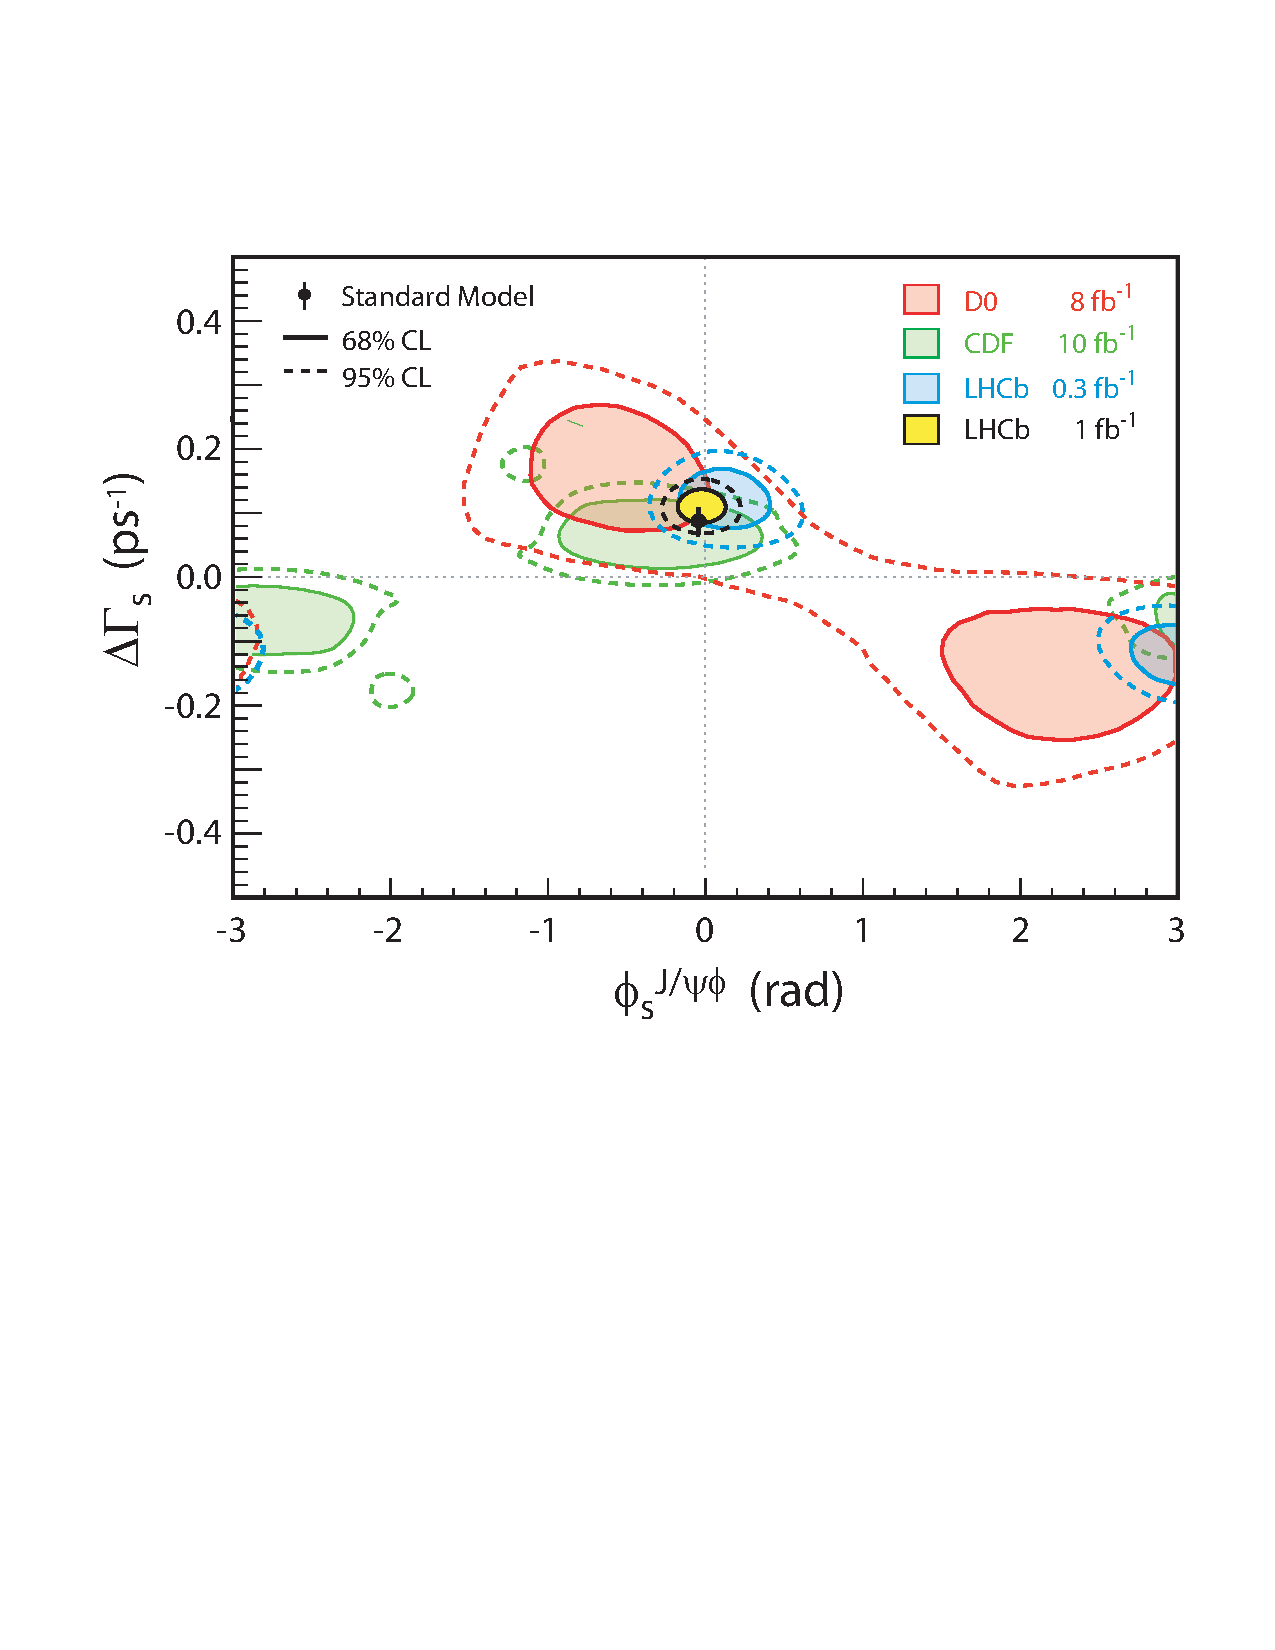
\includegraphics[scale=0.65,bb=50 300 580 700,clip=true]{Roger-plot}
    \vspace*{-1.0cm}
  \end{center}
  \caption{
    \small %captions should be a little bit smaller than main text
    Comparison of our result to those from other experiments.
    Note that the style of this figure differs slightly from that of Figure~\ref{fig:example}}
  \label{fig:roger}
\end{figure}

\clearpage

}

\end{document} 

%
% ****** End of file apssamp.tex ******
